\documentclass[10pt,a4paper]{report}
\usepackage[utf8]{inputenc}
\usepackage{amsmath}
\usepackage{amsfonts}
\usepackage{amssymb}
\usepackage{graphicx}
\usepackage{pdfpages}
\usepackage{color}

\usepackage{hyperref}
\hypersetup{
    colorlinks,
    citecolor=black,
    filecolor=black,
    linkcolor=black,
    urlcolor=black
} 

\author{Helena Brekalo}
\begin{document}


\begin{titlepage}

\newcommand{\HRule}{\rule{\linewidth}{0.5mm}} % Defines a new command for the horizontal lines, change thickness here

\center % Center everything on the page
 
\textsc{\LARGE KU Leuven}\\[1.5cm] % Name of your university/college

\begin{figure}[ht!]
\centering
\includegraphics[width=30mm]{logo_theo.png}
\label{kulogo}
\end{figure}

\textsc{\Large Ma Ingenieurswetenschappen: Computerwetenschappen}\\[0.5cm] % Major heading such as course name


\HRule \\[0.4cm]
{ \huge \bfseries Bedrijfskunde $\&$ Entrepreneurship}\\[0.4cm]
\HRule \\[1.5cm]


\textsc{\Large Lesnota's}\\[0.5cm] % Minor heading such as course title


\large \emph{Author:}\\
Helena \textsc{Brekalo}\\[3cm]

{\large 2015-2016}\\[3cm] % Date

\vfill % Fill the rest of the page with whitespace

\end{titlepage}

\tableofcontents
\clearpage

\section{Dankwoord}
Met dank aan Vincent Van Gestel voor het dumpsterdiven naar oplossingen van oefenzitting 4 en voor het nemen van foto's van de ontbrekende slides tijdens de gastlezing.

\chapter{Les 1}

\section{Slides: 1\_Bedrijfskunde\_Inleiding(1)}

\paragraph{Slide 6:} $\sim$Productlevencyclus: tijd waarin men nieuwe producten verwacht verkort $\&$ men wil steeds meer persoonlijke dingen (vari\"eteit). Zie Figuur \ref{les01_01}.

\begin{figure}[h!]
\centering
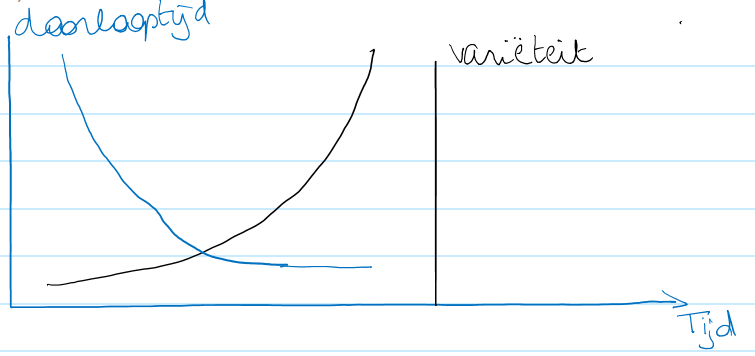
\includegraphics[width=90mm]{Les01_01.png}
\caption{Productlevencyclus} 
\label{les01_01}
\end{figure}

\paragraph{Slide 8:} Bedrijfseconomisch luik: voorspellingstechnieken: je hebt je product en je moet weten hoeveel je de komende maanden en jaren gaat produceren en welke consequenties daaraan hangen.\\
ERP: bv IER en ISP, personeelsbestanden, boekhouding,… 

\paragraph{Slide 10:} Set kleine vraagjes: vooral over begrippen (JIT, MRP,…). Let goed op verwoording en denk goed na over het antwoord! Bv: investering waarbij je 100 000 euro uitgeeft en je krijgt de volgende 5 jaar 30 000 terug, willen we nagaan of het interessant is. Als de waarde van het geld hetzelfde blijft, is het interessant. Kom niet af dat je rekenfouten gemaakt hebt op het examen!

\paragraph{Slide 13 $\&$ 14:}
\begin{itemize}
\item 5000 v.C. daar heeft men een aantal zaken teruggevonden die tonen dat men al bezig was met een soort boekhouding: bijhouden voorraden, leningen, uitgaven,… Daar werden dus al zaken opgevolgd.
\item Egyptische piramides: tonnen stenen moesten aangebracht worden, maar er waren ook enorm veel mensen aan het werken die moesten eten, slapen, verzorgd worden,…
\item 3000v.C.: volledig ontwikkeld staatssysteem.
\item Code van Hammurabi: men sprak al over minimumlonen.
\item Hannibal: logistieke organisatie om met heel die troep over te steken en eten te voorzien.
\item Feodale systemen: hi\"erarchische systemen: keizer met leenheren,… tot aan de lijfeigenen. De keizer kan niet alles voorzien dus gaat die een organisatiestructuur opbouwen die voor hem het best past. Je krijgt dan een baas die een aantal taken delegeert (bv. belastingen heffen, waarvan een deel moet worden afgestaan aan de keizer $\&$ manschappen sturen in tijden van oorlog).
\item 1300: dubbele boekhouding en kostberekeningen.
\item 1436: scheepswerf in Venetië: flowshop (alle producten volgen dezelfde weg: je hebt een aantal stations en men start met een skelet en op het einde heeft men een afgewerkte boot). Dit is zo'n bekend voorbeeld omdat er daar toen 2000 werknemers werkten en die slaagden erin om 100 boten te maken in minder dan 2 maanden. Er was dus een volledige organisatie van de lijn, de toevoer, het eten,…
\item 1700 e.v.: Industri\"ele Revolutie: men bouwde stoommachines etc.: massaproductie. Men is gestart met gespecialiseerde taken, bouwmachines en massaproductie. Uitwisselbare stukken: men kan stukken gebruiken in verschillende machines: minder voorraad van die stukken nodig want je kan ze op meerdere plaatsen gebruiken. Bv kopiemachines: worden al voor 3e of 4e keer gebruikt. Zo'n 80\% van een oude machine is nog bruikbaar en wordt dus hergebruikt.
\item 1886: eerste keer ingenieur als economist $\rightarrow$ industrial engineering.
\item Henri Fayol: je moet denken aan productie, veiligheid, sturen plannen, accountancy,… $\rightarrow$ extra zaken die aan bod komen.
	\end{itemize}
	
\paragraph{Slide 15:} Ondernemen: er zijn mensen, materialen,…\\
Schumpeter: gebruikte de term ``ondernemer'' voor het eerst in de vorm van innovator. \\
Bedrijven worden alsmaar complexer $\&$ de klant komt meer centraal te staan: hij wil meer en sneller. Er wordt ook meer gekeken naar duurzame zaken. 

\paragraph{Slide 16:} Massaproductie etc kan problemen geven (realisatie) $\rightarrow$ biedt kortetermijnwinst. Er is dus langetermijnvisie nodig. \\
Henry Ford: als een bedrijf alleen maar winst wil maken, zou het eigenlijk niet mogen bestaan. Er is ook maatschappelijke bijdrage,… nodig. Toen is men de zaken anders beginnen bekijken.\\
Club van Rome: we moeten op een andere manier tewerk gaan om ervoor te zorgen dat we nog een paar 100 jaar kunnen voortgaan.

\paragraph{Slide 17:} Men moet duurzaam werken en men moet proberen voldoen aan de noden van vandaag op zo'n manier dat we de toekomst niet compromiteren.

\paragraph{Slide 19 - 22:} Veel bedrijven willen meewerken aan duurzaamheid. Als je hun jaarverslagen neemt, zie je dat ze daar ook over duurzaamheid praten.

\paragraph{Slide 23:} Een bedrijf staat niet op zichzelf dus je moet kijken naar de positie van de onderneming. Verschillende standpunten: gebruikers (mensen die producten aankopen: hebben bepaalde verwachtingen), de maatschappij (werkgelegenheid gewenst, diensten die iets voor hen doen), verwachtingen van het individu, markten (concurrenten!).\\
Een bedrijf is een economisch maar ook een sociaal systeem: zie \textbf{Slide 24:} aandachtspunten van Lotus op het sociaal systeem.

\paragraph{Slide 25:} Een bedrijf moet een meerwaarde cre\"eren, afkomstig van inkomsten en en uitgaven. Het verschil tussen beide is de meerwaarde. Je gebruikt die meerwaarde om lonen te betalen, belastingen, vergoeding voor het kapitaal, leningen $\&$ autofinanciering (kan gebruikt worden voor investeringen,…).

\paragraph{Slide 26:} Het bedrijf staat tussen leveranciers en klanten. Alle pijltjes zijn dingen die belangrijk zijn, bv levenscyclus: waar bevindt mijn product zich in de markt, wat is zijn levenscyclus?\\ Macht: ben je een grote klant van de leverancier of de enige klant? Dan kun je een aantal zaken doordrukken. Als je maar een kleine leverancier bent, dan zal dat minder zijn.

\paragraph{Slide 30:} Je kan intrapreneurship hebben (binnen een bedrijf) of erbuiten (entrepreneurship). In beide gevallen zoekt men naar innovatie. Schumpeter dacht dat dat vooral kon gevonden worden binnen bedrijven omdat er daar meer geld beschikbaar was. Dat is niet het geval. Naarmate een bedrijf groter wordt, wordt de organisatiestructuur logger en idee\"en die van werknemers komen, komen vaak niet tot ``boven''. In kleine bedrijven komt dat dus meer boven. Mensen die goede idee\"en hebben over aangepaste producten kunnen dat in een box steken in sommige bedrijven en zo gaat men die idee\"en evalueren.

\paragraph{Slide 31:} Een idee moet goed zijn en je moet ervoor zorgen dat de klant dat wil. Normaal moet het zo zijn dat jouw product het probleem van een klant oplost. Het moet een product zijn met duidelijke specificaties en het moet een potenti\"ele markt hebben. Ook rekening houden met concurrentie (bv. wasmachinetablet: vroeger was dat alleen maar in poeder en toen kwam Finish met tabletten en die begonnen 3 maand op voorhand daar reclame voor te maken. 1 week nadat het op de markt was gekomen, kwam een copycat er ook mee op de markt om dus ook een graantje mee te pikken. Het grote voordeel was dat de reclame gemaakt werd door Finish). Je moet voldoende beginkapitaal hebben (zelf hebben, binnenbrengen door investeerders aan te spreken,…). Je moet de juiste mensen aantrekken.

\section{Slides: 2\_Bedrijfskunde\_wat is een bedrijf}

\paragraph{Slide 5:} Er kunnen verschillende standpunten ingenomen worden om te kijken naar bedrijven. 

\paragraph{Slide 6:} De 4 sectoren: 2 laatste samen (tertiaire en kwartaire). De primaire sector neemt zo'n 3\% van BNP in beslag, de secundaire 33\% en de tertiaire en kwartaire de rest. De maatschappij is volledig veranderd van agrarisch naar dienstverlening.

\paragraph{Slide 7:} Je kan het bedrijf in 2 delen splitsen: goederen en diensten. De manier van werken en plannen is hier dikwijls anders. Als je kijkt naar ziekenhuizen, zij leveren ook diensten, dat is nog een stap verder dan hier. Als je naar een bank gaat voor een lening, negoti\"eer je. Als je naar een ziekenhuis gaat voor een operatie, ben je een product want je ondergaat de operatie. 

\paragraph{Slide 11 $\&$ 12:} Aangezien je beperkt aansprakelijk bent, word je veel meer gecontroleerd op wat je doet. 

\paragraph{Slide 13 e.v.:} Voor welk soort bedrijven.

\chapter{Les 2}

\section{Slides: 2\_Bedrijfskunde\_wat is een bedrijf}

\paragraph{Slide 19:} Onder kleine onderneming valt ook leverancier van brandstoffen (flexibeler).

\paragraph{Slide 23:} Interne jaarrekening: voor eigen gebruik.

\paragraph{Slide 24:} Marktstructuur: als je met een nieuw product op de markt wil komen, moet je rekening houden met het type markt. Als je kijkt naar volkomen concurrentie (een 100-tal spelers op de markt en de prijs wordt bepaald door de markt), als je daar op de markt wil komen, gaat niemand daar een probleem van maken (je moet gewoon zorgen dat kostprijs $>$ productieprijs). Bij een monopolie is dat anders: 1 partij bepaalt de prijs (op zo'n manier dat hij voldoende winst kan maken). Als er dan iemand op de markt komt met een gelijkaardig product, gaat de monopolist zijn prijzen laten dalen op zo'n manier dat hij bijna zeker is dat de nieuwkomer het product niet aan die prijzen kan produceren (de monopolist kan in grote volumes produceren, de binnenkomer zeer waarschijnlijk nog niet). Bij een oligopolie zijn er een beperkt aantal spelers die de markt be\"invloeden. Daar binnengeraken is ook moeilijk, maar minder moeilijk dan bij een monopolie. Monopolistische concurrentie: afzetten van andere producenten door middel van productdifferentiatie.\\
$\Rightarrow$ Kijken hoe je je bedrijf moet organiseren om op de markt te kunnen komen.

\paragraph{Slide 25 e.v.:} Hoofdstuk 7 van Technische bedrijfsvoering $\&$ organisatie.

\paragraph{Slide 27:} Normaal heb je ergens een bepaalde visie, missie, strategie. Je gaat die dingen zo organiseren om je doelen te bereiken. Als je focust op verschillende producten moet je structuur dat ook weergeven.\\
Er zijn een aantal taken in verband met productie, verkoop en marketing $\rightarrow$ verantwoordelijkheden toewijzen en kijken hoe die zaken met elkaar communiceren.

\paragraph{Slide 28:} Organisatiehandleiding: taak- $\&$ functieomschrijving: elk bedrijf moet dat dus hebben. Ook bij KULeuven (onderwijsraad). Voor elke groep/functie bestaat dat. Ieder krijgt een instructieset met taken voor zijn/haar functie. Bij audits worden al die zaken ook gecontroleerd.

\paragraph{Slide 29:} Organisatieschema: bovenaan: algemeen directeur en per karakteristiek/element van het bedrijf een aantal afdelingen die uitgebouwd zijn. De personen die in een bepaalde silo zitten, gaan niet direct met andere mensen uit andere silo's spreken, dat zal via via verlopen.

\paragraph{Slide 31:} Lijnorganisatie = volledig hi\"erarchisch. Een persoon onder een bepaalde persoon moet alleen luisteren naar die persoon en niet naar andere hogere functies waar hij/zij niet onder staat. $\rightarrow$ Duidelijke verantwoordelijkheidsbegrenzing: je gaat niet buiten je eigen gebied.

\paragraph{Slide 32:} Co\"ordinatie: als een uitvoerder naar een ``andere" baas moet gaan, zal dat via zijn baas moeten, dan naar directeur en zo naar die andere baas: grote omweg.
Zo'n structuur zal regelmatig wijzigen, is een levend organisme.\\
Omspanningsvermogen: hoeveel mensen kan ik overzien? Als je als afdelingshoofd makkelijk 15 mensen kunt opvolgen, maar als uw afdeling tot 25 mensen omvat, moet je die misschien beter opsplitsen.\\
Spanwijdte: hoeveel mensen heb ik te overzien? Als spanwijdte $>$ omspanningsvermogen: beter op te splitsen.

\paragraph{Slide 33 $\&$ 34:} Speciale functie: staffunctie: ondersteunende functie (neemt zelf geen beslissingen, alleen raad en advies en schrijft documenten zodat een van de managers/directeurs dat kan gebruiken om bepaalde dingen door te drukken/voeren). Die verzamelt informatie, op systematische manier neerschrijven zodat de manager tot een besluit kan komen. Voordeel: het is nog steeds de manager/baas die beslist, de stafmederwerker neemt zelf geen beslissingen.

\paragraph{Slide 35:} Nadelen: draagt geen verantwoordelijkheden (de directeur is nog steeds de verantwoordelijke), het kan zijn dat je een fout overwicht krijgt: dat hij teveel overwicht krijgt op de manager.\\
Stafrelaties zijn voor advies, functionele relaties: diensten die dezelfde functiedeskundigheid hebben (bv. administratie). Men probeert binnen een bedrijf allemaal dezelfde documenten te gebruiken zodat die standaard zijn en makkelijk door te geven zijn zodat alles voor iedereen duidelijk is. Vroeger kon iedereen de dingen uitschrijven zoals men wou, tegenwoordig gaat dat niet meer, er zijn standaarden en het is voor iedereen hetzelfde.

\paragraph{Slide 37:} Een afdeling/bedrijf verandert qua structuur (bv. meer werknemers) en het overzien wordt misschien moeilijker. Decentralisatie is nodig wanneer dat beter past voor het type bedrijf om bepaalde zaken beter te kunnen uitvoeren. Soms is het beter eerst te decentraliseren en dan lokaal weer te centraliseren. $\rightarrow$ Je gaat alles mixen met elkaar.

\paragraph{Slide 41:} Functionele structuur: met departementen werken.

\paragraph{Slide 48:} Voordeel: groep mensen die gekoppeld zijn aan een project zelf. Nadeel: dubbele functies.

\paragraph{Slide 50:} Men laat de functionele structuur bestaan (mensen zitten in afdelingen), maar men gaat gebruik maken van die mensen op een horizontale manier. Voor projecten pikt men er dan mensen uit. Die mensen hebben nog altijd hun normale taken met daarbovenop extra taken voor het project (\textbf{Slide 53}). Matrixstructuur: verticale en horizontale taken.

\paragraph{Slide 54:} Men probeert meer en meer samen te werken (vroeger: leverancier was evil, wou gewoon winst maken). Men maakt speciale afspraken (bv. met VMI: Vendor Managed Inventory $\rightarrow$ de leverancier en het bedrijf werken samen. De leverancier weet hoeveel stukken er in het magazijn liggen en die kent het productieplan van het bedrijf (de klant) en kan zo zelf beslissen wanneer hij het magazijn gaat aanvullen wanneer dat het beste past in zijn planning. Moet er wel altijd voor zorgen dat er genoeg stukken liggen in het magazijn. De klant betaalt alleen voor wat hij gebruikt. Op die manier kan de leverancier zich beter organiseren. Bedrijven gaan elkaar soms ook overnemen om bepaalde zaken uit te voeren.\\
Horizontaal: leveranciers gaan samenwerken (bv. luchtvaartmaatschappijen: wisselstukken worden samen bekeken).

\paragraph{Slide 57:} Als je kijkt naar bedrijven, daar zijn een aantal functies (operations, marketing en finance). Die 3 moeten altijd op mekaar afgestemd zijn, anders raak je in de problemen. Bv. Apple: op een bepaald moment maakten ze reclame over het feit dat iedereen met een Apple kon werken. Dit sprak veel mensen aan en iedereen begon dat te bestellen. De computers werden geleverd (steeds met meer vertraging). Men dacht dat er een stijging ging zijn van de verkoop, maar marketing had het opgezet zonder te informeren bij de managers en financing. Men is veel gaan verkopen, maar men kon niet leveren. Er was dus geen cash flow. Men begon met de productie, maar omdat men dat te laat wist, kwam er een tekort waarbij men tot 6 maand moest wachten voor de pc geleverd kon worden. Zie Figuur \ref{les02_01}.


\begin{figure}[h!]
\centering
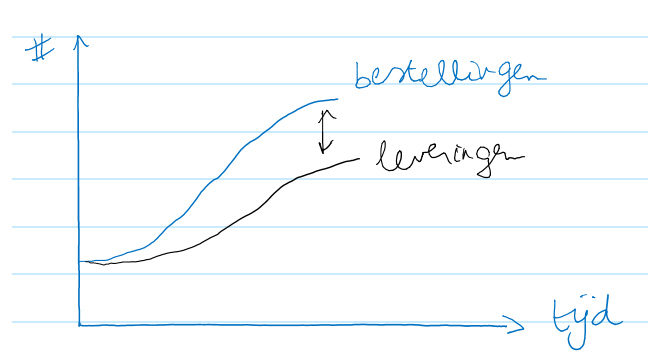
\includegraphics[width=90mm]{Les02_01.png}
\caption{Productlevencyclus} 
\label{les02_01}
\end{figure}


Dit was slechte reclame voor Apple: het was dan wel makkelijk om mee te werken, maar men moest er een half jaar op wachten.

\paragraph{Slide 58:} Bij massaproductie gaat men een lijn ontwikkelen om een bepaald product te ontwikkelen (bv. Ford Genk). Intermittent productie: het een is eenmalig, het ander is een grote batch. We hebben producten A, B, C waarbij een aantal stuks gemaakt moet worden. De productie moet zo gebeuren dat de voorraad beperkt is en de omstellingen die gemaakt moeten worden ook beperkt zijn. Je kan grote batches maken om minder omstellingen te hebben, maar dan heb je grote voorraden. Als je kleine voorraden maakt (dus kleine batches), heb je meer omstellingen en heb je te weinig tijd. De twee zijn dus tegenovergesteld aan elkaar. Je moet dit gaan optimaliseren.

\paragraph{Slide 59:} Strategische planning gaat kijken naar de impact op lange termijn (neemt niet per s\'e veel tijd in beslag!). Je moet kijken naar de tijdshorizon en zo objectieven vastleggen. Er is een hoge graad van onzekerheid omdat je over langere periodes gaat kijken, je weet niet altijd wat er juist gaat gebeuren. Het kan zijn dat men vrij goed kan voorspellen wat het verbruik gaat zijn bij klanten, maar niet per s\'e.\\
Tactische planning: wat als de verkoop cyclisch is: hoe ga je produceren? Ook cyclisch, of aan constante hoeveelheden? Zie Figuur \ref{les02_02}.


\begin{figure}[h!]
\centering
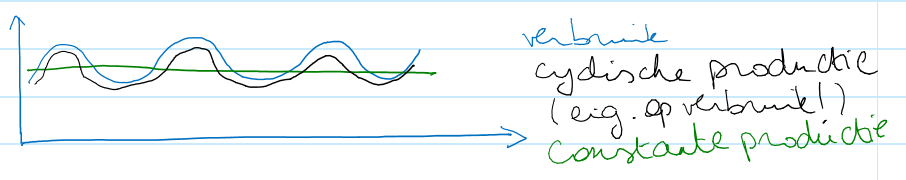
\includegraphics[width=90mm]{Les02_02.png}
\caption{Productlevencyclus} 
\label{les02_02}
\end{figure}


Normaal wordt eerst de strategische planning vastgelegd, dan tactische en dan operationele, maar het is niet puur sequentieel, het kan zijn dat men soms terugkoppelt en zaken aanpast.

\section{Slides: 3\_Bedrijfskunde\_Productlevenscyclus}

\paragraph{Slide 3:} Meestal komen producten er op basis van market pull, maar soms ook door de technologie zelf. Klanten vragen vaak zelf wel (market pull). Bij technology push gaat men proberen om noden te cre\"eren bij de klanten.

\paragraph{Slide 4:} De verschillende fasen: 
\begin{enumerate}
\item Introductie: product op de markt brengen. Hierbij is het dikwijls zo dat niemand het heeft en je moet dus zelf een prijs gaan bepalen. Als je zeker bent dat niemand het meteen gaat kopen, dan kan je de prijs relatief hoog zetten en meteen winst maken. Als het vervangbaar is door andere producten, is dat moeilijker. Als je start met een product is uw machinepark niet altijd correct afgesteld. Het product wordt dus vaak verkocht met verlies. Daarna kan je wel winst beginnen maken natuurlijk. 
\item Vroege groei: je moet nog oppassen voor copycats! 
\item Late groei: je moet je proberen differenti\"eren van andere bedrijven. Uw groei zal minder steil zijn omdat er bv. concurrentie op de markt komt. Je zal dus minder verandering hebben, maar je moet ook kijken naar productie en financi\"en. Distributie komt hier ook bij kijken omdat je moet leveren aan de klanten.
\item Maturiteit: iedereen heeft het product en wat gekocht wordt is vervanging. Dan probeer je nog differentiatie te maken.
\item Eindstuk: iedereen is het product beu want er is een beter product op de markt, dus je kan verlies gaan lijden. Soms kan je hier geluk hebben: door je kostenstructuur te wijzigen kan je nog op een goede manier verkopen, ook als de verkoop daalt. Het kan dus zijn dat de interesse daalt, maar de marktpositie groeit nog wel.
\end{enumerate}

\paragraph{Slide 6:} Normaal, als je kijkt naar bedrijven die eerst op de markt zijn, die krijgen het grootste marktaandeel. Op de slide heb je bv. de cyclus van een bepaald product (PLC(1)), die ligt hoger dan die van PLC(2). 

\paragraph{Slide 7:} Men kan ook proberen van de levenscyclus te verlengen door er andere karakteristieken aan te geven. Bv. plakband: nieuwe versie op de markt brengen zodat het makkelijk af te scheuren is of zoiets. Zo ook met sigaretten bv. (met filter, minder teer,…).

\paragraph{Slide 8:} Niet alle curves lopen altijd hetzelfde: foothill: men brengt een product op de markt en sommige mensen moeten het dan hebben omdat het net op de markt is. Dan plots stopt het want niet iedereen is zeker of het interessant is of niet. Men wacht dan af wat de reactie is van de mensen die het al gekocht hebben. Het kan dan zijn dat het terug naar boven gaat (want positieve reacties van mensen die al gekocht hebben), of dat het niet goed is en dan daalt de curve (snel).

\paragraph{Slide 9:} Modeproducten: bv. geboorte prinses in Engeland: alle merchandise daarrond wordt enorm veel gekocht, iets later ineens niet meer. Hetzelfde verhaal met de hoolahoop.

\paragraph{Slide 10:} Grondstoffen en energiebronnen: hun gebruik is constant (olie, rubber, steenkool,…), ze zitten al lang in de maturiteitsfase.

\paragraph{Slide 11:} Als in de maturiteitsfase: flowshop maken dat specifiek gericht is op dat product. 
Je moet er rekening mee houden dat de PLC steeds korter worden, soms zijn producten al verouderd tegen dat ze op de markt komen.

\chapter{Les 3}

\section{Slides: 4\_algemene boekhouding} 

\paragraph{Slide 1} Bij een bedrijf moet je altijd een 5-jarig plan opstellen.

\paragraph{Slide 3:} We hebben een balans nodig omdat we willen weten wat er gebeurd is in het voorbije jaar. Een balans zit op strategisch niveau omdat we op lange termijn gaan kijken. Elk bedrijf moet zijn balans neerleggen bij de bank van Belgi\"e, maar vaak stelt men een tussentijdse balans op (bv. om de 3 maanden), zo kan men sneller ingrijpen indien nodig. \\
De bedoeling van algemene boekhouding is dat je ziet wat er juist gebeurd is binnen het bedrijf. Het is altijd van belang dat er een evenwicht is ($\sim$balans): we halen geld binnen (bronnen) en dat geld gebruiken we binnen ons bedrijf. De som van wat er binnenkomt moet gelijk zijn aan de som van wat we gebruiken.\\
Er zijn verschillende activiteiten die doorgaan tijdens een jaar (gewerkt, machinekosten,…) en we willen nagaan of die winstgevend zijn $\rightarrow$ resultatenrekening om te kijken of er winst gemaakt is of niet. Dan beslissen wat je met die winst gaat doen (uitkeren aan de aandeelhouders, uitgeven aan nieuwe investeringen,…).

\paragraph{Slide 4:} Figuur die het ondernemingsgebeuren weergeeft. Normaal is het zo dat als we willen produceren, we middelen moeten gebruiken om die productie te doen. Aan de ene kant interne middelen (mensen, machines) en aan de andere kant externe middelen (grondstoffen, gebruiksgoederen die zijn aangekocht). Deze middelen bepalen de kostprijs van ons product. Een deel van de middelen komt er via het verkopen van het product. Je moet weten wat de kostprijs is, welke winst je wil hebben en welke verkoopprijs je wilt. Deze laatste moet zo zijn dat je rekening houdt met uw positie in de markt.\\ Uiteindelijk komt het geld terug binnen (middelen voortgebracht door de activiteit).
Die geldstroom is enorm belangrijk: nodig om te investeren.

\paragraph{Slide 5:} We hebben een balans en resultatenrekening en we willen een samenvatting geven van wat er gebeurd is tijdens het jaar. We willen weten wat er gebeurd ismet de bezittingen en de vorderingen en het kapitaal.
Om de zaak aan te sturen zijn er de twee belangrijke principes.

\paragraph{Slide 6:} Je kan vanuit verschillende standpunten kijken naar een bedrijf (vanuit eigenaarsperspectief, banken,…).

\paragraph{Slide 7:} We hebben altijd een schuld tegenover eigenaars: zie Figuur \ref{les03_01}.

\begin{figure}[h!]
\centering
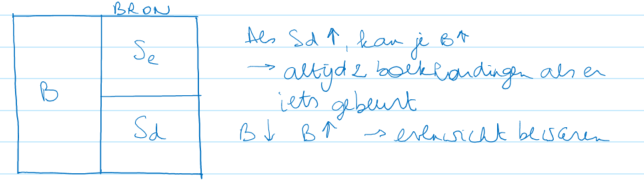
\includegraphics[width=90mm]{Les03_01.png}
\caption{Les 3 Slide 7} 
\label{les03_01}
\end{figure}

\paragraph{Slide 8:} De balans geeft altijd de zaken weer op een bepaald tijdstip (``foto"). Tussen 2 balansen (zoals hierboven getekend) heb je de resultatenrekening (geeft weer wat de activiteiten waren) en het journaal (houdt alles bij wat er gebeurt tussen 2 balansen). De balans is dus een momentopname, de resultatenrekening geeft meer de overgang aan.

\paragraph{Slide 9:} Balans: in een bepaalde volgorde (zie volgende slide). De passivazijde: staat gerangschikt volgens eisbaarheidsgraad. Het eigen vermogen is wat de personen die het bedrijf hebben opgericht hebben binnengebracht. Dat blijft in het bedrijf tot het bedrijf er eventueel mee stopt. Hoe verder naar beneden in de lijst, hoe sneller je die instantie moet terugbetalen.

\paragraph{Slide 11:} Als je kijkt naar een balans, moet dat op verschillende manieren: per kolom (anders bij dienstenbedrijven dan bij productiebedrijven). Het hangt er deels vanaf wat je gaat doen met uw winst. Je kan die bij de reserves gaan plaatsen (dan moet je die niet gaan uitbetalen), of aan dividenden (dan moet je dat uitbetalen aan de aandeelhouders). Als je de winst uitbetaalt, moet je 2000 terugbetalen op korte termijn. In principe zijn er genoeg middelen om de 2000 op korte termijn terug te betalen.
Je moet ook kijken over de tijdshorizon: naar de balans van dit jaar en van vorig jaar,… zo kan je evoluties binnen het bedrijf zien.

\paragraph{Slide 12:} Balansen van hetzelfde bedrijf, bekeken op verschillende tijdstippen. Het bedrijf werkt met seizoensgebonden vraag waarschijnlijk. Als je een piek hebt, moet je uw productieactiviteit daar niet naar aanpassen, je moet gewoon voorraad opbouwen in de magerdere periode (bv speelgoed): zie Figuur \ref{les03_02}.

\begin{figure}[h!]
\centering
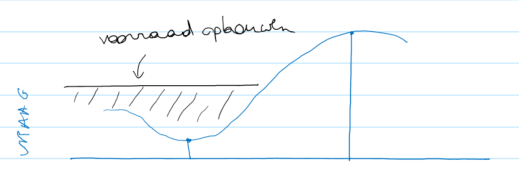
\includegraphics[width=90mm]{Les03_02.png}
\caption{Les 3 Slide 12} 
\label{les03_02}
\end{figure}

Je kan dus een totaal verschillend beeld krijgen wanneer je naar verschillende momenten in het jaar kijkt. 

\paragraph{Slide 13:} Je moet zorgen dat de balans eenduidig/juist is $\rightarrow$ wettelijke voorschriften.
\begin{itemize}
\item Informatiebron voor de bedrijfsleiding: keuzes etc.
\item Informatiebron voor diverse categorie\"en ge\"interesseerden: bv voor investeerders.
\end{itemize}
Als je een bedrijf opricht, moet je een ondernemingsplan oprichten en aantonen aan de bank dat je voldoende middelen hebt om de komende 5 jaar door te komen en dat je de interesten en aflossingen kunt afbetalen.
De overheid krijgt belastingen en als het goed gaat met het bedrijf zijn er werknemers die geen steun nodig hebben (en zij betalen ook belastingen).

\paragraph{Slide 14:} Er staan veel posten op de balans en die moeten op de juiste manier geschat worden.
\begin{itemize} 
\item Bedrijven kunnen hier laks in zijn, zeker als het gaat over financi\"ele activa (fluctueren dagelijks op de beurzen). 
\item Balanseenheid: moet eenduidig zijn en altijd hetzelfde stramien volgen. Als je lineair afschrijft (elk jaar hetzelfde bedrag), dan moet je dat elk jaar hetzelfde doen. Hetzelfde met de waardering van de voorraden. Eenmaal je gestart bent met een bepaalde regel, moet je die aanhouden $\rightarrow$ consistentie tussen verschillende balansen! Als je de regel wil aanpassen, moet je een aangepaste balans van vorig jaar geven zodat het opnieuw vergeleken kan worden.
\item Balansklaarheid: het moet duidelijk zijn wat er onder elke post staat. Als je een balans bekijkt heb je 2-3 pagina's overzicht en een 30-tal pagina's met verduidelijkingen van wat er juist bedoeld wordt.
\end{itemize}

\paragraph{Slide 15:} De sociale context is meer en meer aan het groeien.

\paragraph{Slide 17:} Zie Figuur \ref{les03_03}.

\begin{figure}[h!]
\centering
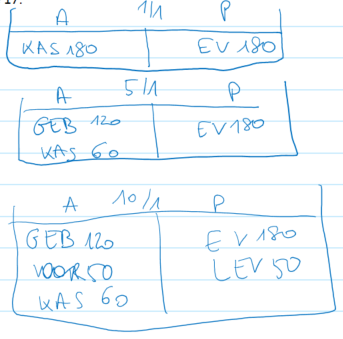
\includegraphics[width=50mm]{Les03_03.png}
\caption{Les 3 Slide 17} 
\label{les03_03}
\end{figure}

\paragraph{Slide 18:} Links altijd debet, rechts altijd credit (geheugensteuntje: denk aan prof zijn initialen).

\paragraph{Slide 19:} Creditzijde stijgt als we de bron laten stijgen (passiefzijde).

\paragraph{Slide 20:} Resultatenrekening: kostenrekening en opbrengstenrekeningen: alles opgeteld. Opbrengst: credit + wat je aan de schuldeisers moet terugbetalen (je krijgt iets).

\paragraph{Slide 21:} Journaalboek waarbij alle transacties worden neergeschreven.

\paragraph{Slide 22:} Balans: alle boeken samenbrengen en alle saldi nemen en plaatsen in de balans en de resultatenrekening.

\paragraph{Slide 24 $\&$ 25:}
\begin{enumerate}
\item 2 posten: kas (dus kasboek nodig) en kapitaal.
\item Er wordt niet gespecifi\"eerd waar het geld terecht komt, dus we zetten het in de kas.
\item Er worden obligaties gekocht met geld uit de kas.
\item We hebben kosten gemaakt om producten aan te kopen, maar we hebben een voorraad en deltavoorraad liggen en 4 transacties. Alles in verband met voorraad en deltavoorraad wordt meestal apart gehouden. Wordt achteraf bekeken, rekening houdend met de waardering op dat momemt.
\end{enumerate}

Zie Figuur \ref{les03_04}, \ref{les03_05} $\&$ \ref{les03_06}.

\begin{figure}[h!]
\centering
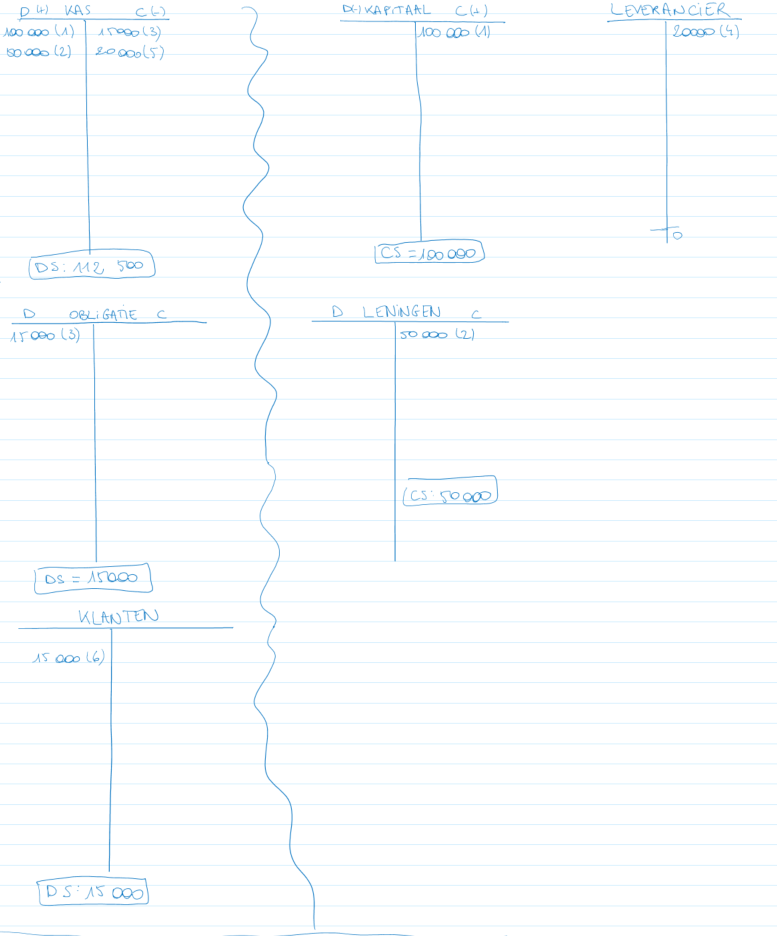
\includegraphics[width=120mm]{Les03_04.png}
\caption{Les 3 Slide 24 $\&$ 25} 
\label{les03_04}
\end{figure}

\begin{figure}[h!]
\centering
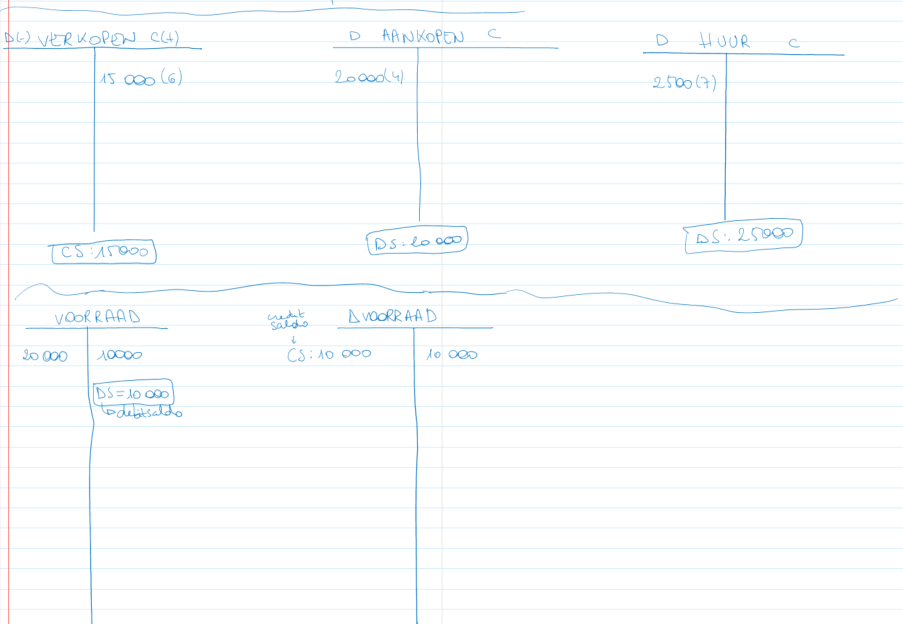
\includegraphics[width=120mm]{Les03_05.png}
\caption{Les 3 Slide 24 $\&$ 25} 
\label{les03_05}
\end{figure}

\begin{figure}[h!]
\centering
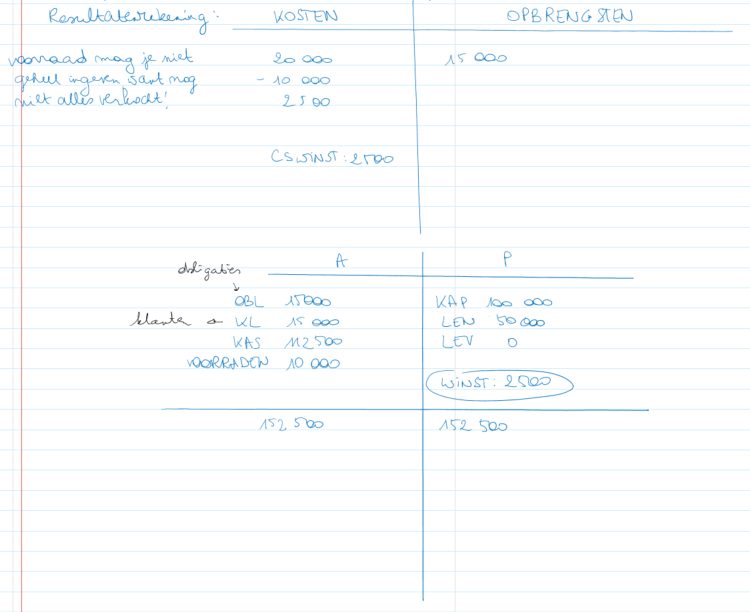
\includegraphics[width=120mm]{Les03_06.png}
\caption{Les 3 Slide 24 $\&$ 25} 
\label{les03_06}
\end{figure}

\paragraph{Slide 31:} Opgelet met voorraden: soms kan je de indruk krijgen dat je veel winst maakt terwijl dat niet zo is.

\paragraph{Slide 34:} Eerst wordt de resultatenrekening doorgerekend en dan wordt de nettowinst bekomen en die kan je opdelen in gereserveerde en verdeelde winst.

\section{Slides: 5\_Bedrijfskunde\_Financiele analyse en financiering}

\paragraph{Slide 2:} Men wil een balans tussen de eisbaarheid en de (liquiditeits-?)graad.\\
De ratio-analyse is niet voor alle bedrijven hetzelfde, goed kijken naar de sector!\\
Financiering: we willen ervoor zorgen dat we voldoende cashflow hebben.

\paragraph{Slide 3: }
\begin{itemize}
\item Beleggers: ge\"interesseerd in beleggingen en kapitaalwinsten.
\item Schuldeisers willen hun geld terug, zijn ge\"interesseerd in rentabiliteit en de schuldenstructuur (als veel schulden: gaan niet direct willen investeren).
\end{itemize}

\chapter{Les 4}

\section{Slides: 5\_Bedrijfskunde\_Financiele analyse en financiering}

\paragraph{Slide 4:} Wij gaan naar de laatste 2 kijken.

\paragraph{Slide 5:} De actiefzijde en passiefzijde wijzigen op een jaar en je wil weten hoe dat gebeurd is, welke stromen voor die veranderingen hebben gezorgd.

\paragraph{Slide 6:} Figuur die ons vertelt hoe de kasstromen in elkaar zitten. Beneden is er de kas en daar kunnen er dingen de kas binnenkomen en verlaten.

\paragraph{Slide 7:} Als we kijken naar de balansen kunnen we ook kijken naar de mutatiebalans. We krijgen enkel de balans en geen omschrijving van wat er tijdens het jaar is gebeurd. We willen weten wat er is gebeurd met de activa en passiva. Kijken we naar materi\"ele vaste activa, zien we dat het bedrag met 250 gestegen is: er is een investering gebeurd (geld ergens vandaan gehaald en dat geld aangewend). Handelsvorderingen zijn ook gestegen: we verwachten nu nog meer geld terug van onze klanten (geld zit bij de klant). De voorraden zijn gedaald. Aanwending: stijging van de kosten, bron: daling.\\
Passiefkant: schulden op meer dan 1 jaar: die zijn gestegen: we hebben ergens meer geld binnengehaald en dat is een bron van inkomsten. De schulden $<$ 1 jaar zijn gedaald (die zijn terugbetaald). Als een bron stijgt, stijgen de passiva.\\
Ook van belang is een aanwending van 250 vaste activa.

\paragraph{Slide 8:} Let op: de totalen zijn gelijk aan die van in \textbf{Slide 7}!

\paragraph{Slide 9:} We gaan sterktes en zwaktes proberen afleiden op basis van ratio's (kengetallen). Je kan die ratio's ook overheen de tijd bekijken en tussen verschillende ondernemingen maar wel best binnen dezelfde sector.

\paragraph{Slide 10:} We willen dat de kanten aan elkaar gelijk zijn (ook binnen de hokjes zelf, niet alleen in totaal), zo willen we bv. dat we onze schulden zo snel mogelijk kunnen terugbetalen. 

\paragraph{Slide 11:} Schulden op korte termijn terugbetaald en we hebben zo nog 80 overgehouden: er zijn reserves.

\paragraph{Slide 12:} In \textbf{Slide 10} hebben we een bedrijfskapitaal van 0 omdat we alles nodig hebben om de schulden terug te betalen. In \textbf{Slide 11} is het bedrijfskapitaal 80 omdat er dus nog over is.\\
Relatieve vorm: geeft de vergelijking aan. Als die groter is dan 1, is het bedrijfskapitaal dus positief.\\

\paragraph{Slide 13:} Je krijgt uw geld pas op het einde van de onderste lijn terug: je moet heel die periode dus overbruggen. Hoe langer die periode, hoe slechter voor je bedrijf. Je kan die inkorten door de productie sneller te laten worden, de voorraden kleiner te laten worden, leverancierskrediet groter te maken of het klantenkrediet kleiner te maken. Kan die periode negatief worden? Ja, bv. in winkels. Bedrijven als Colruyt hebben meestal contracten van 60 tot 90 dagen (dus na 90 dagen betalen ze de leveranciers). De voorraad ligt er meestal 2 weken (dus 14 dagen). De klant betaalt meteen (dus na 14 dagen). Dit wilt zeggen dat de winkels geld hebben ontvangen voor dingen die ze zelf nog niet hebben afbetaald. Zie Figuur \ref{les04_01}

\begin{figure}[h!]
\centering
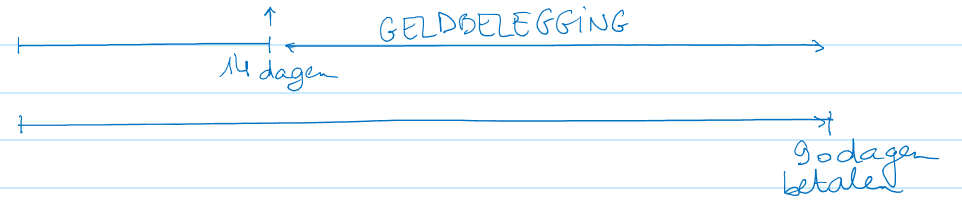
\includegraphics[width=90mm]{Les04_01.png}
\caption{Les 4 Slide 13} 
\label{les04_01}
\end{figure}

\paragraph{Slide 14:} Voorraadrotatie willen we liefst hoog, dan hebben we een kleine gemiddelde voorraad, dus deze roteert snel. We gaan de voorraad in het bedrijf inkorten (op de tekening hierboven zou het dus ook maar een aantal dagen zijn). Bv. zie Figuur \ref{les04_02}.

\begin{figure}[h!]
\centering
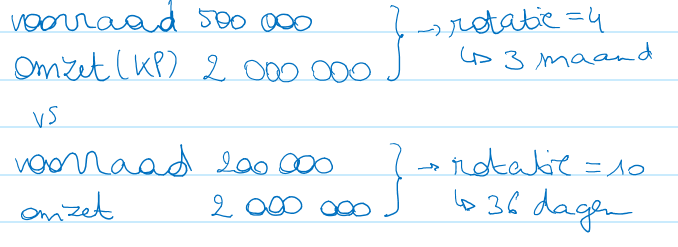
\includegraphics[width=90mm]{Les04_02.png}
\caption{Les 4 Slide 14} 
\label{les04_02}
\end{figure}

Klantenrotatie ($\sim \frac{1}{\text{klantenkrediet}}$) willen we zo groot mogelijk hebben (dan betalen ze sneller), leveranciersrotatie willen we zo laag mogelijk (later leveranciers betalen). \\
Als je kijkt naar de tapijtindustrie en de voorraadperiode (VP),  het leverancierskrediet (LK) en het klantenkrediet (KK), dan liggen de tapijten er meestal 75 dagen, de leveranciers worden na 83 dagen betaald en de klanten betalen na 85 dagen. In tabelvorm:


\begin{table}[h!]
\centering
\begin{tabular}{|c||c|c|c|}
\hline                         										
		 				&	VP 		&	LK		&	KK		\\	\hline	\hline
Tapijt					&	75		&	83		&	85		\\	\hline
Kleinhandel Voeding		&	29		&	61		&	10		\\	\hline

\end{tabular}
\label{les4_slide14}
\end{table}

\paragraph{Slide 15:} Schuldenratio moet zo laag mogelijk zijn (niet teveel vertrouwen op externe financiering), solvabiliteitsratio moet zo hoog mogelijk zijn.\\
Toegevoegde waarde: deze wordt gebruikt om lonen te betalen, de staat te betalen,…

\paragraph{Slide 16:} De autofinanciering is interessant: kan gebruikt worden om verdere financieringen door te voeren.

\paragraph{Slide 17:} Afschrijvingen worden afgeschreven als kost maar ze zijn geen cash flow. Als je een investering doet van 1 miljoen, betaal je dat en gedurende de volgende jaren mag je bv. 100 000 afschrijven. Dit is een recuperatie van gemaakte investeringskosten, maar dat is dus geen nieuw geld dat binnenkomt.

\paragraph{Slide 21:} Grafisch voorstellen van wat daar ook staat: zie Figuur \ref{les04_03}.

\begin{figure}[h!]
\centering
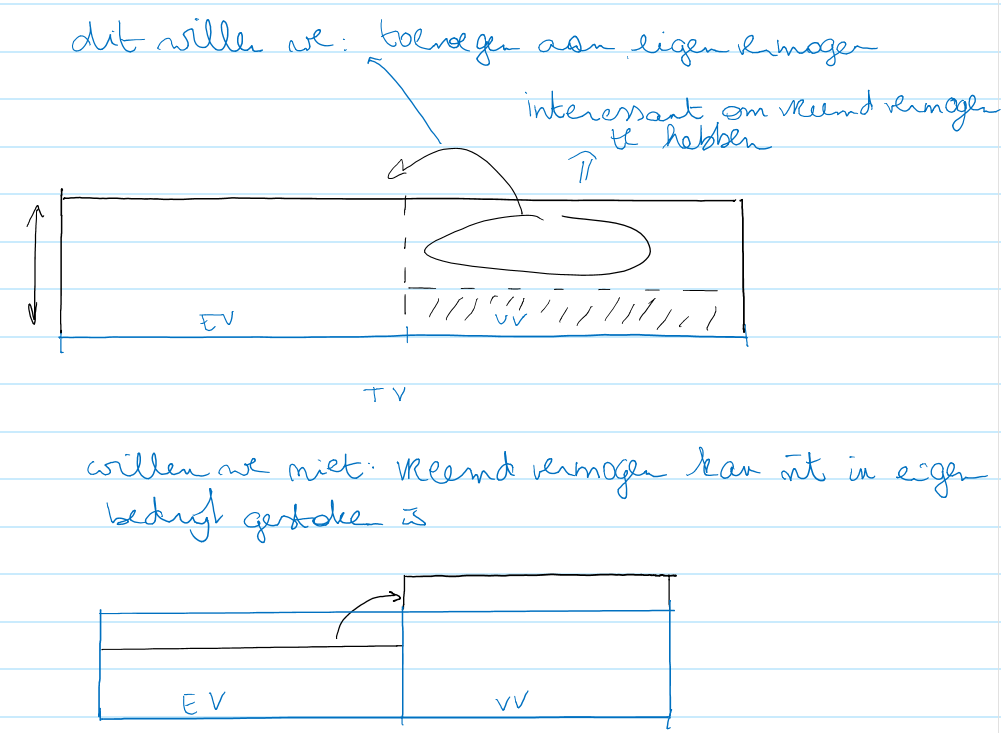
\includegraphics[width=90mm]{Les04_03.png}
\caption{Les 4 Slide 21} 
\label{les04_03}
\end{figure}

\paragraph{Slide 22:} Balans op 31/12 die jaren x en x+1 toont.

\paragraph{Slide 23:} Zie Figuur \ref{les04_04}, \ref{les04_05} $\&$ \ref{les04_06}.

\begin{figure}[h!]
\centering
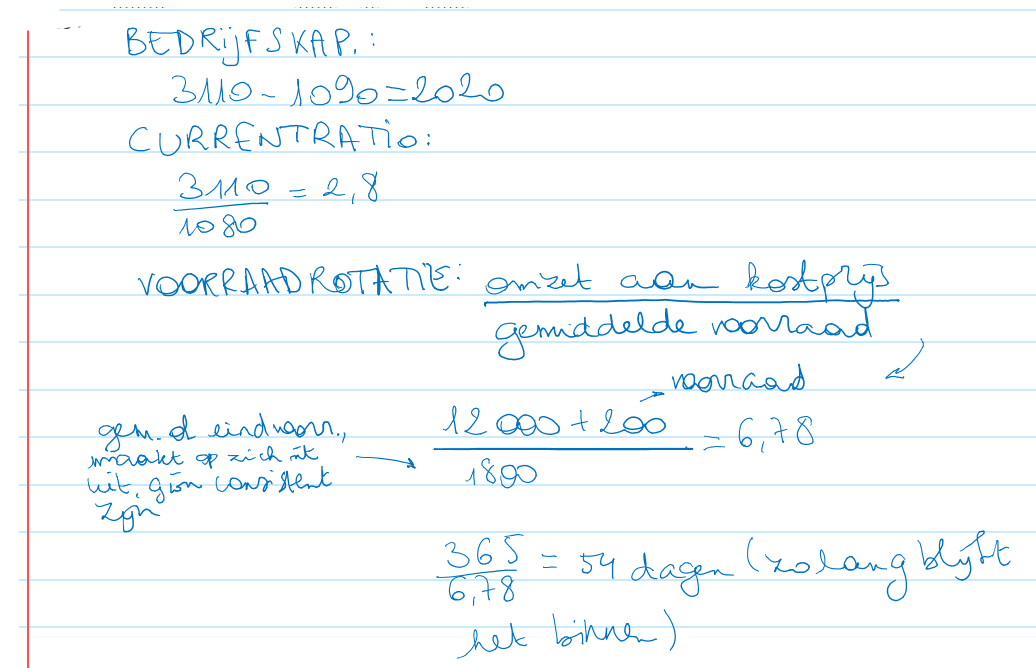
\includegraphics[width=90mm]{Les04_04.png}
\caption{Les 4 Slide 23} 
\label{les04_04}
\end{figure}

\begin{figure}[h!]
\centering
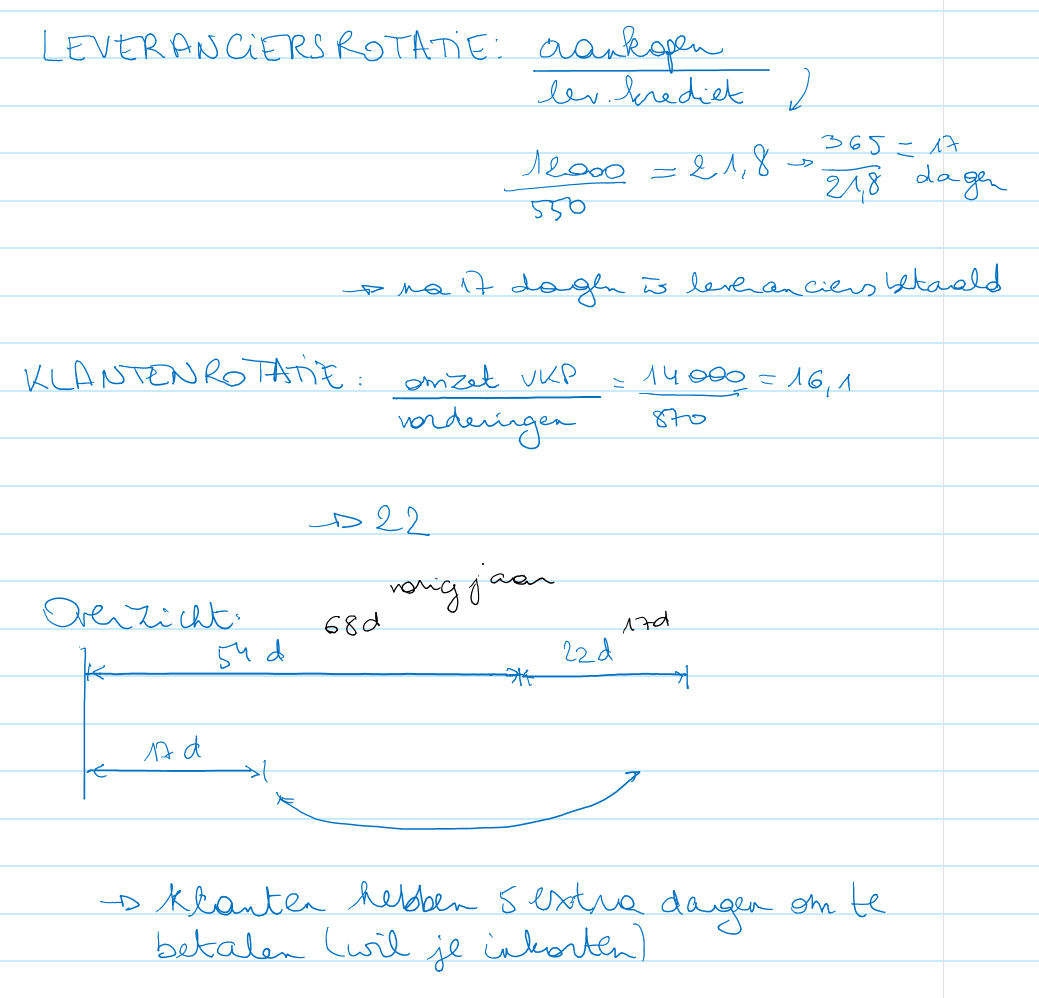
\includegraphics[width=90mm]{Les04_05.png}
\caption{Les 4 Slide 23} 
\label{les04_05}
\end{figure}

\begin{figure}[h!]
\centering
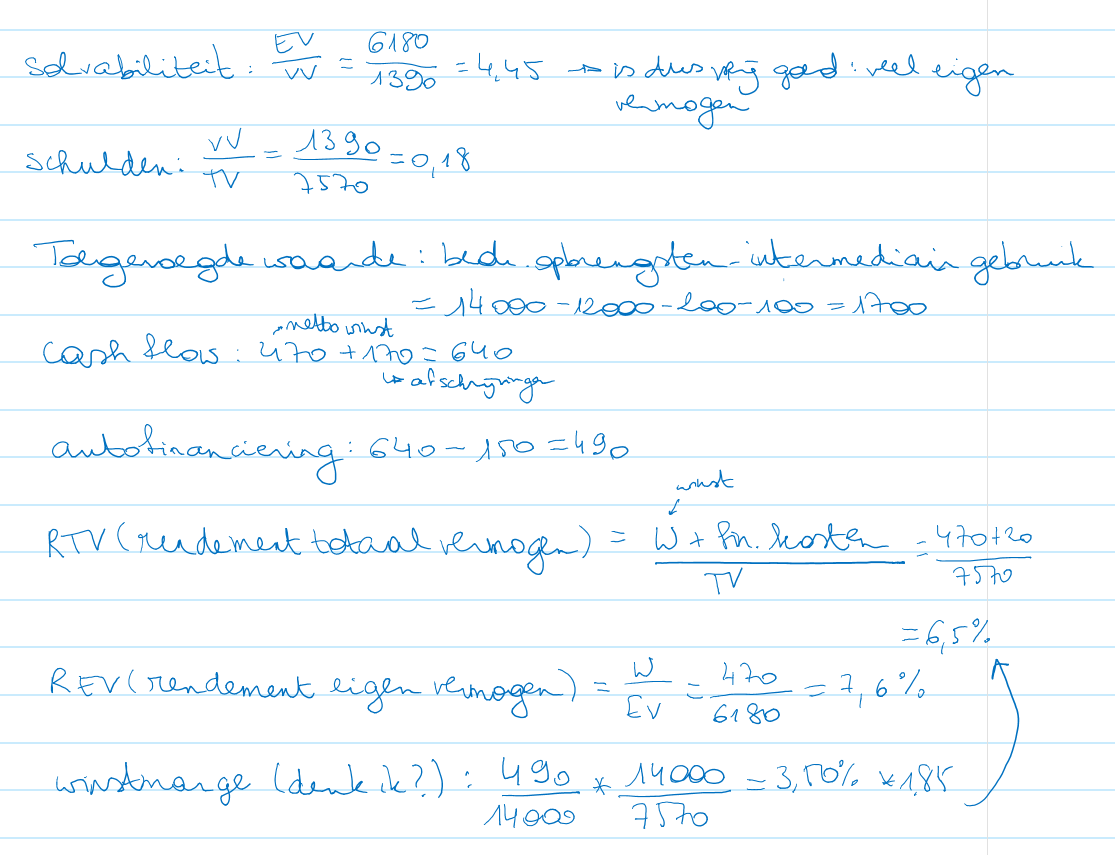
\includegraphics[width=110mm]{Les04_06.png}
\caption{Les 4 Slide 23} 
\label{les04_06}
\end{figure}

\paragraph{Slide 25:} Je moet elk jaar beslissen of je dividenden gaat uitbetalen of niet (staat dus niet vast). Obligaties moeten terugbetaald worden, aandelen niet.

\paragraph{Slide 26:} Rekening-courant: je hebt x euro staan en naarmate je daar gebruik van maakt, zoveel interest betaal je daarop.

\chapter{Les 5}

\section{Slides: 6\_Bedrijfskunde\_Kostprijssystemen}

\paragraph{Slide 3:} Structuurbeslissingen: investeringen doen, deze hebben invloed op de kostprijs. Het is de bedoeling dat we de kost kennen van elk product (maar dit is niet eenduidig!).\\
Kostenbeheer van elke afdeling: elke afdeling heeft vaste kosten en variabele kosten. We willen zien of deze zaken optimaal worden ingezet.

\paragraph{Slide 4:} Voor ons is het eerste puntje minder interessant. Wij zijn meer ge\"interesseerd in puntje 2 $\&$ 3. Toewijsbaarheid: als je denkt aan de grondstoffen en daar is een product van gemaakt, wil je weten hoeveel grondstoffen daar naartoe zijn gegaan.

\paragraph{Slide 5:} Je kan uw elementen opsplitsen. Het meest rechtse is een combinatie van het linkse en het middelste. Vaste indirecte kosten: bv. gebouwen (je kan niet meteen zeggen voor welk product dat gebouw dient). Let op: als we spreken over indirecte kosten, gaat het normaal over een bedrijf dat meer dan 1 product maakt. Als het bedrijf maar 1 product maakt, is alles direct toewijsbaar, heb je geen indirecte kosten.

\paragraph{Slide 6:} Bij vaste kosten maakt het niet uit hoeveel producten je maakt, de kosten blijven hetzelfde.

\paragraph{Slide 7:} Er kan een sprong inzitten, bv. omdat uw magazijn te klein is geworden, dus verhuis je naar een groter magazijn, maar dan wordt uw kost weer vast.

\paragraph{Slide 8:} Variabele kosten: die zullen meestal proportioneel zijn met de productie. Soms kan het zijn dat er een extra stijging is als je dicht bij de maximale capaciteit zit (progressief). Het kan ook zijn dat je een afname hebt wanneer je bv. grondstoffen moet aankopen en bij het aankopen van grote batches krijg je korting (degressief). 

\paragraph{Slide 9:}
\begin{itemize}
\item Directe kosten: zijn rechtstreeks toewijsbaar. Voorraden moet je wel apart houden omdat je rekening moet houden met de voorraadwaardering.
\item Directe materiaalkosten: we werken hier met FIFO (we kijken naar de oudste producten eerst en we kijken ook naar de waarde van de grondstoffen op dat moment) en LIFO (omgekeerd).
\end{itemize}

\paragraph{Slide 10:} Je gaat bij t2 maar 1000 aankopen in plaats van meteen 2000.

\paragraph{Slide 11:} Identiek dezelfde aankopen en verkopen, maar de 4000 van t3 wordt eerst uit t2 en t1 genomen.\\
Afhankelijk van de situatie (moet vermeld staan op de balans) moet je rekening houden met wat je doet.\\
FIFO en LIFO is puur boekhoudkundig! Als we dus met LIFO werken en we hebben een bedrijf dat yoghurt verkoopt, wil dat niet zeggen dat ze alleen de meest verse zullen verkopen. Boekhoudkundig zal er misschien wel LIFO gebruikt worden, maar fysisch FIFO.

\paragraph{Slide 12:} Je kan verschillende manieren gebruiken, maar je moet altijd consistent zijn en het moet ergens neergeschreven staan.

\paragraph{Slide 13:} Als iemand aan een bepaalde productielijn staat, weet je waar dat geld naartoe gaat. \\
Indirecte kosten: moeilijker om toe te wijzen. Je moet uitvissen waarom je een kost zou toewijzen aan een bepaald proces of product. Vroeger kon men zeggen dat 90\% van de kosten direct toewijsbaar was (kleine fout). Als je nu gaat kijken naar bedrijven, is dat sterk veranderd: meer dan de helft van de kosten zijn nu indirecte kosten. Vandaar dat je ook grotere afwijkingen kunt krijgen op uw kosten.

\paragraph{Slide 14:}
\begin{itemize}
\item Primitieve toeslagmethode:
\begin{itemize}
\item We kunnen kijken naar de directe loonkosten als dat de belangrijkste parameter is binnen het bedrijf. 
\item Per eenheid eindproductie: we maken van alles samen 5000 stuks, deel indirecte kosten door 5000 en verdeel het.
\item Toeslag op basis van directe materiaalkosten: indirecte kosten zijn gerelateerd aan de directe materiaalkosten of (lonen?).
\item Op basis van directe kosten: som van beide.
\end{itemize}
\item Verfijnde toeslagmethoden: indirecte kosten meer en meer proberen uitsplitsen.
\end{itemize}

\paragraph{Slide 15:} Ondersteuningscentra: proberen toewijzen aan de hoofdcentra. Laatste: kan je niet meteen toewijzen. Zie kader rechts.

\paragraph{Slide 16:} Voorbeeld: smederij: cijfers achter rode lijn zijn niet meegeteld in het totaal (naast sleutel).
\% directe lonen: je gaat je indirecte lonen berekenen aan de hand van een percentage van de directe lonen (ongeveer 1/8 hier: alle indirecte lonen zullen ongeveer 1/8 van de directe lonen zijn).

\paragraph{Slide 17:} Zie Figuur \ref{les05_01}, \ref{les05_02} $\&$ \ref{les05_03}.

\begin{figure}[h!]
\centering
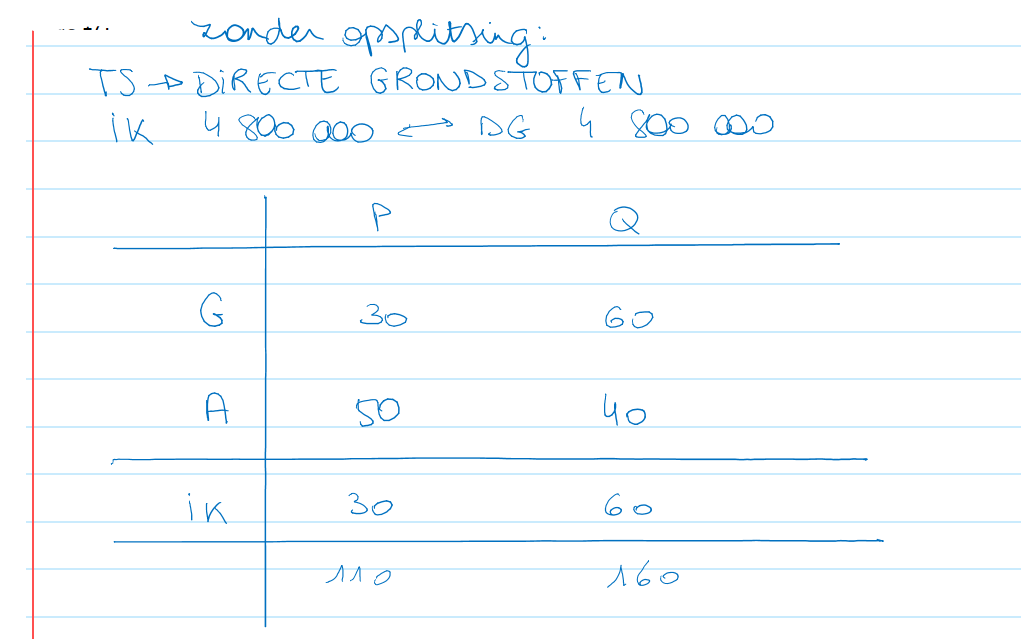
\includegraphics[width=90mm]{Les05_01.png}
\caption{Les 5 Slide 17} 
\label{les05_01}
\end{figure}

\begin{figure}[h!]
\centering
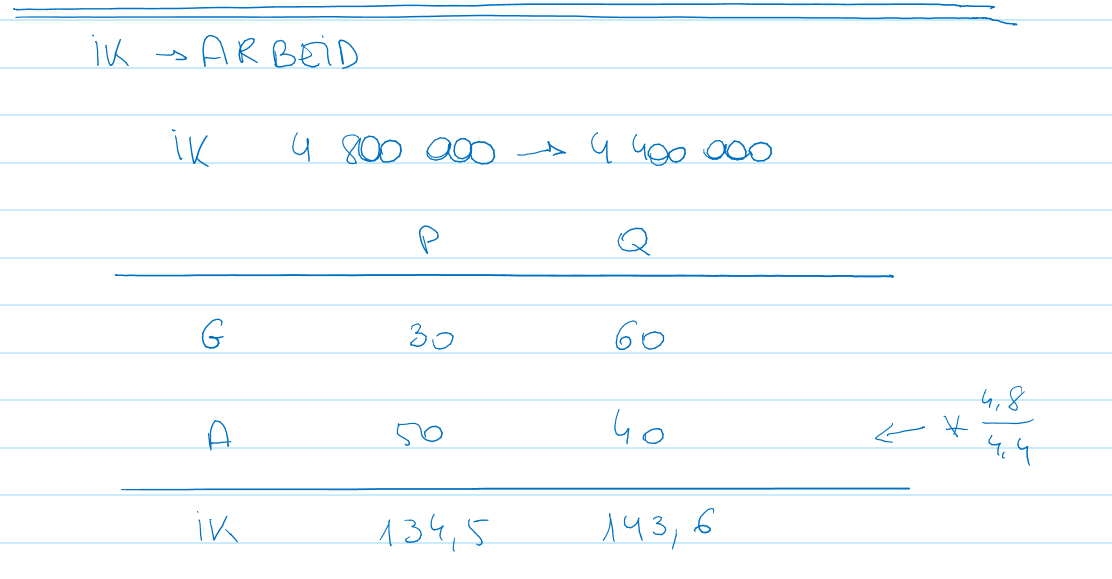
\includegraphics[width=90mm]{Les05_02.png}
\caption{Les 5 Slide 17} 
\label{les05_02}
\end{figure}

\begin{figure}[h!]
\centering
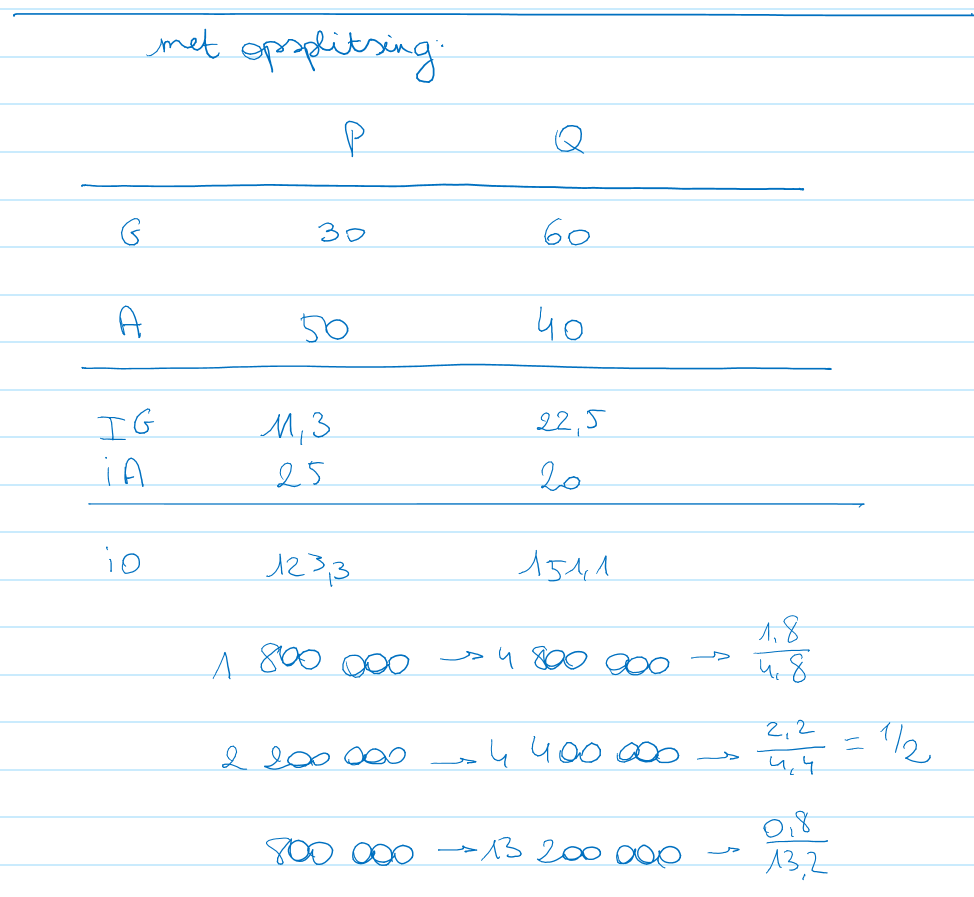
\includegraphics[width=90mm]{Les05_03.png}
\caption{Les 5 Slide 17} 
\label{les05_03}
\end{figure}

\paragraph{Slide 21:} 250 000: eerste getal vermenigvuldigd met 40 000 en het tweede getal vermenigvuldigd met 60 000.

\paragraph{Slide 22:} Zie Figuur \ref{les05_04}.

\begin{figure}[h!]
\centering
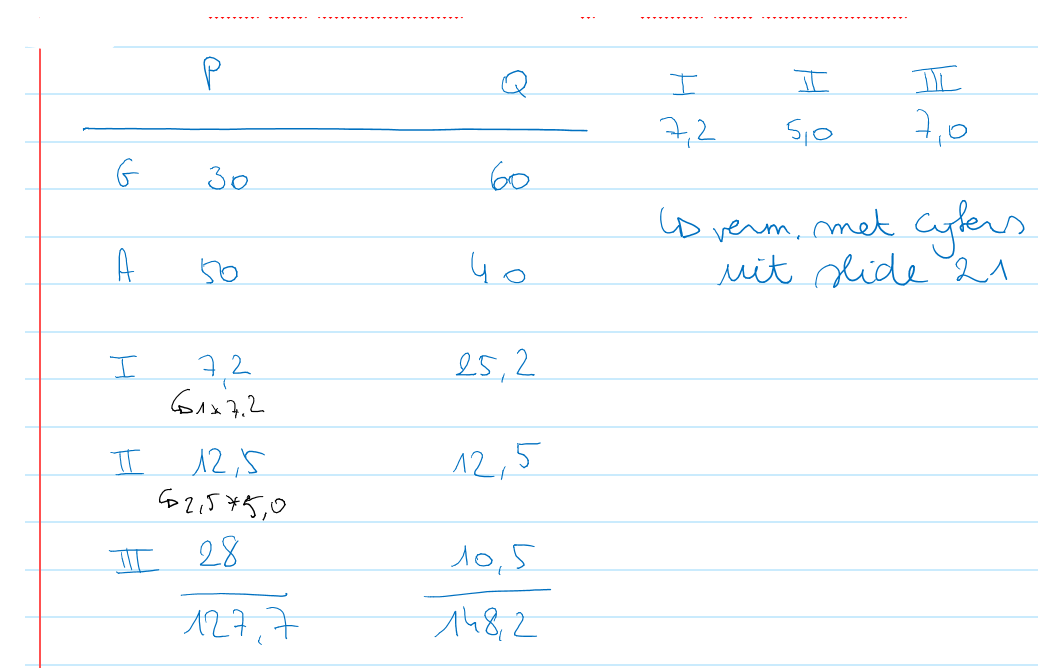
\includegraphics[width=90mm]{Les05_04.png}
\caption{Les 5 Slide 22} 
\label{les05_04}
\end{figure}

\paragraph{Slide 24:} Als je een bepaalde investering doet, wordt dat niet onmiddelijk ingebracht. Je brengt achteraf afschrijvingen in (gebouw, machine,…). De kasstroom gebeurt op het moment van investeren. Je hebt verschillende definities zoals getoond op de slide.

\paragraph{Slide 25:} Zie Figuur \ref{les05_05}.


\begin{figure}[h!]
\centering
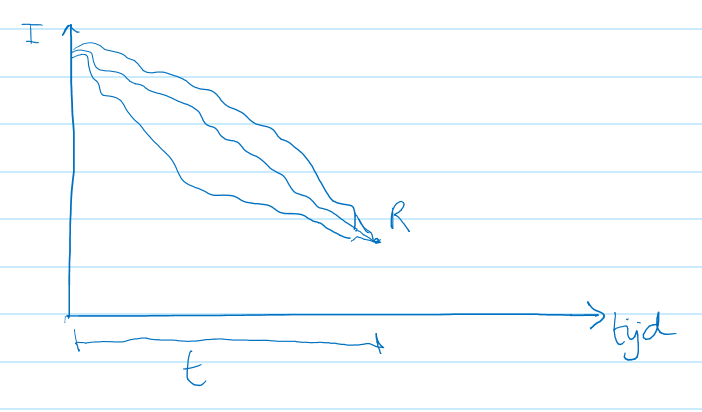
\includegraphics[width=90mm]{Les05_05.png}
\caption{Les 5 Slide 25} 
\label{les05_05}
\end{figure}

\paragraph{Slide 27:} Afschrijvingsperiode: kan vari\"eren: voor machines kan dat 5 jaar zijn, voor gebouwen 30 jaar. Hangt ook af van de fysische of technische levensduur: een wagen kan bv. afgeschreven worden na 5 jaar. %Economische levensduur: de machine (???)
%Fiscale levensduur

\paragraph{Slide 28:} Lineair afschrijven: bepaald investeringsbedrag, product gaat 10 jaar mee. Zie Figuur \ref{les05_06}.

\begin{figure}[h!]
\centering
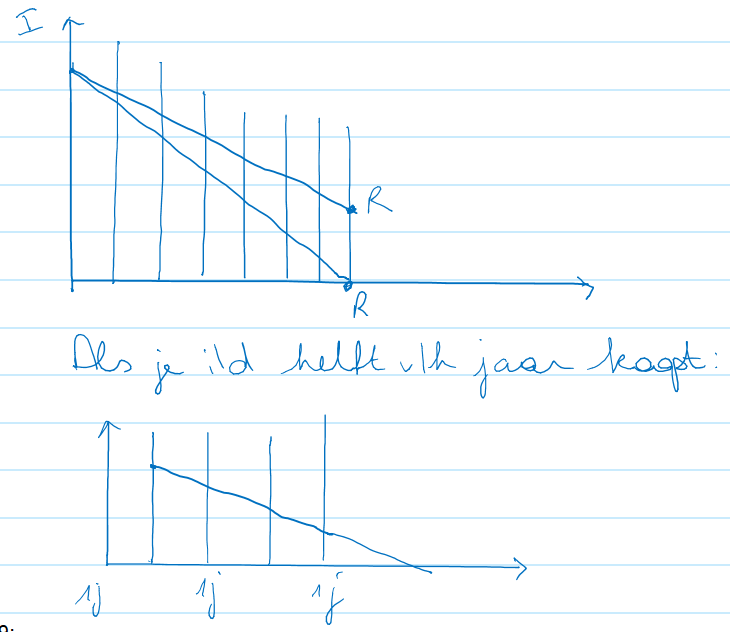
\includegraphics[width=90mm]{Les05_06.png}
\caption{Les 5 Slide 28} 
\label{les05_06}
\end{figure}

\paragraph{Slide 29:} Zie Figuur \ref{les05_07}.

\begin{figure}[h!]
\centering
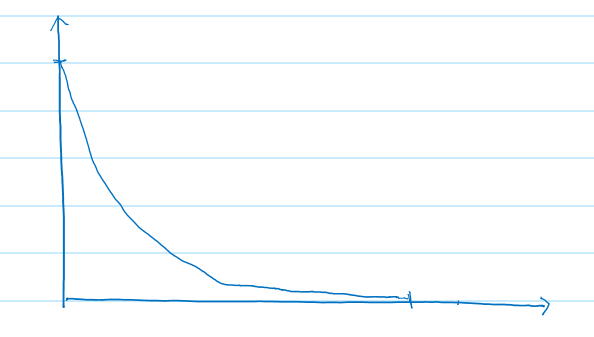
\includegraphics[width=90mm]{Les05_07.png}
\caption{Les 5 Slide 29} 
\label{les05_07}
\end{figure}

\paragraph{Slide 30:} Voorbeeld: elk jaar schrijven we 100 af. Ook mogelijk: zie Figuur \ref{les05_08}.

\begin{figure}[h!]
\centering
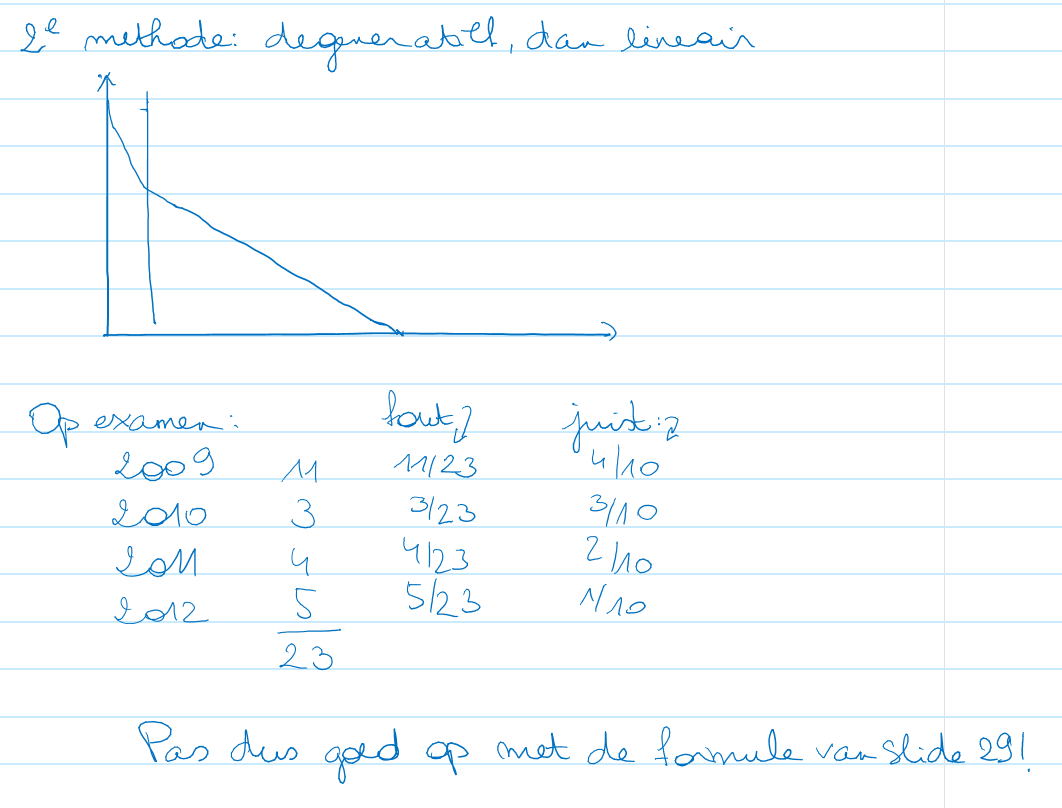
\includegraphics[width=90mm]{Les05_08.png}
\caption{Les 5 Slide 30} 
\label{les05_08}
\end{figure}

\paragraph{Slide 31:}
\begin{itemize}
\item Klassieke totale kostprijs: daar zit alles in (zeg dus niet dat er zaken niet inzitten).
\item Industri\"ele kostprijs: bevat alleen de productiekosten: alle kosten zonder algemene kosten en verkoop.
\item Evenredige kostprijs: enkel de kosten die evenredig zijn met de hoeveelheid van elk product. Deze is dus de kleinste, de industri\"ele kosten zijn al wat hoger en de klassieke kosten zijn de hoogste.
\end{itemize}

\paragraph{Slide 32:} De historische totale kostprijs kan je maar bepalen als alles gebeurd is. Normaal moet je alle postenkosten kennen. Daarom spreekt men over de historische totale kostprijs. Bij industri\"ele en evenredige standaardkostprijs gaat men kijken naar de toekomst.

\paragraph{Slide 34:} Er zijn altijd voor- en nadelen! Afhankelijk van de seizoensperiode kunnen de prijzen vari\"eren omdat men meer/minder stuks maakt. Historisch komt eigenlijk te laat.\\
Ook vervelend: doordat men alles gaat optellen weet je niet goed van waar het allemaal komt. Je hebt dus ook geen verantwoordelijke.

\paragraph{Slide 35:} Als je een full cost berekend hebt, hoe moet je die gaan vergelijken met de kostprijs? Als je variabele kosten van 50 hebt en vaste kosten van 50 en een full cost van 100, terwijl de verkoopprijs 90 is, dan is dat geen slechte zaak. Je moet altijd zorgen dat de verkoopprijs groter is dan uw variabele kost. De vaste kosten zijn toegewezen aan een aantal producten dat je maakt. Als je meer producten gaat produceren, gaan die totale vaste kosten dalen.\\ Normaal hebben we een vaste kost en een variabele kost. Als we een aantal stuks produceren, dan is de totale kost aangeduid op de tekening (1) en de full kost is (2). Als we tot de conclusie komen dat we een verkoopprijs hebben die eronder ligt (3), dan maken we verlies. Als we meer stuks kunnen verkopen en produceren kunnen we wel nog aan winst komen. Zolang de verkoopprijs groter is dan de variabele kosten, wordt nog altijd een deel van de variabele kosten gedekt. Zie Figuur \ref{les05_09}.

\begin{figure}[h!]
\centering
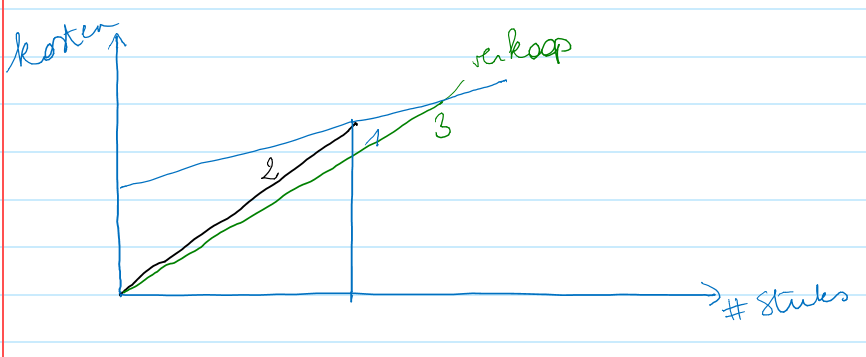
\includegraphics[width=90mm]{Les05_09.png}
\caption{Les 5 Slide 35} 
\label{les05_09}
\end{figure}

\paragraph{Slide 36:} B niet meer verkopen zal ervoor zorgen dat A ook niet meer rendabel is. Het ligt aan uw kostentoewijzing (denk ik).

\paragraph{Slide 39:} Industri\"ele standaardkostprijs: ontstaan op basis van kostenplaatsmethode en standaarden van technische gegevens. Je gaat een schatting maken, dus er zal een verschil zijn tussen de geschatte en de werkelijke kostprijs. Je gaat alles in detail analyseren. 

\paragraph{Slide 40:} Tabel van daarnet.

\paragraph{Slide 41:} Administratieve zaken en verkoop zitten niet in de industri\"ele standaardkostprijs (laatste kolom op \textbf{Slide 40}).

\paragraph{Slide 44:} Er wordt enkel naar de variabele kosten gekeken en die gaan we toewijzen aan kostendragers. Vaste kosten worden naar de resultatenrekening afgevoerd.

\paragraph{Slide 45:} Voordelen:
\begin{itemize}
\item Er wordt een expliciete relatie tussen volumes, kosten en winst gemaakt.
\item Je kan kijken of je korting gaat geven aan een bepaalde klant: je weet wat de marges zijn.
\item Kostencontrole wordt makkelijk.
\end{itemize}

\paragraph{Slide 46:} Prijzen niet altijd laten dalen want dan kan het zijn dat de vaste kosten niet meer gedekt worden. Je mag de vaste kosten dus niet uit het oog verliezen, die zijn er natuurlijk nog altijd.\\
Stel je hebt product A en B. A geeft 3 euro winst per stuk en B 7 euro. Je gaat dus B meer maken en proberen verkopen (intu\"itief). Je weet niet hoeveel uur je nodig hebt om beide te produceren (stel A heeft slechts 1 uur nodig en B 30 uur, dan is A interessanter). Pas dus op met de evenredige kostprijs!

\paragraph{Slide 47:} Je hebt uw vaste kosten (verticale as tot aan C(q) en de variabele kosten OC(q). Zodra je meer produceert dan q* maak je winst. 

\paragraph{Slide 48:} Je moet altijd zorgen dat je kostenstructuur goed zit. Hotels hebben bv. veel vaste kosten. Dit zorgt voor een andere gevoeligheid van het dode punt. Je kan ook verschillende snijpunten krijgen, zie \textbf{Slide 49}.

\paragraph{Slide 49:} Als de vaste kosten een sprong krijgen, kan het dode punt verschuiven. Het kan zijn dat de kostenstructuur van de variabele kosten niet altijd lineair verloopt, maar dicht ligt aan de capaciteitskosten en dat je bv. overuren moet doen en dan kan je dus meer kosten hebben.

\chapter{Les 6: Oefenzitting 1}
\section{Slides: Oefenzitting 1(1)}
Zie volgende pagina voor handgeschreven nota's.

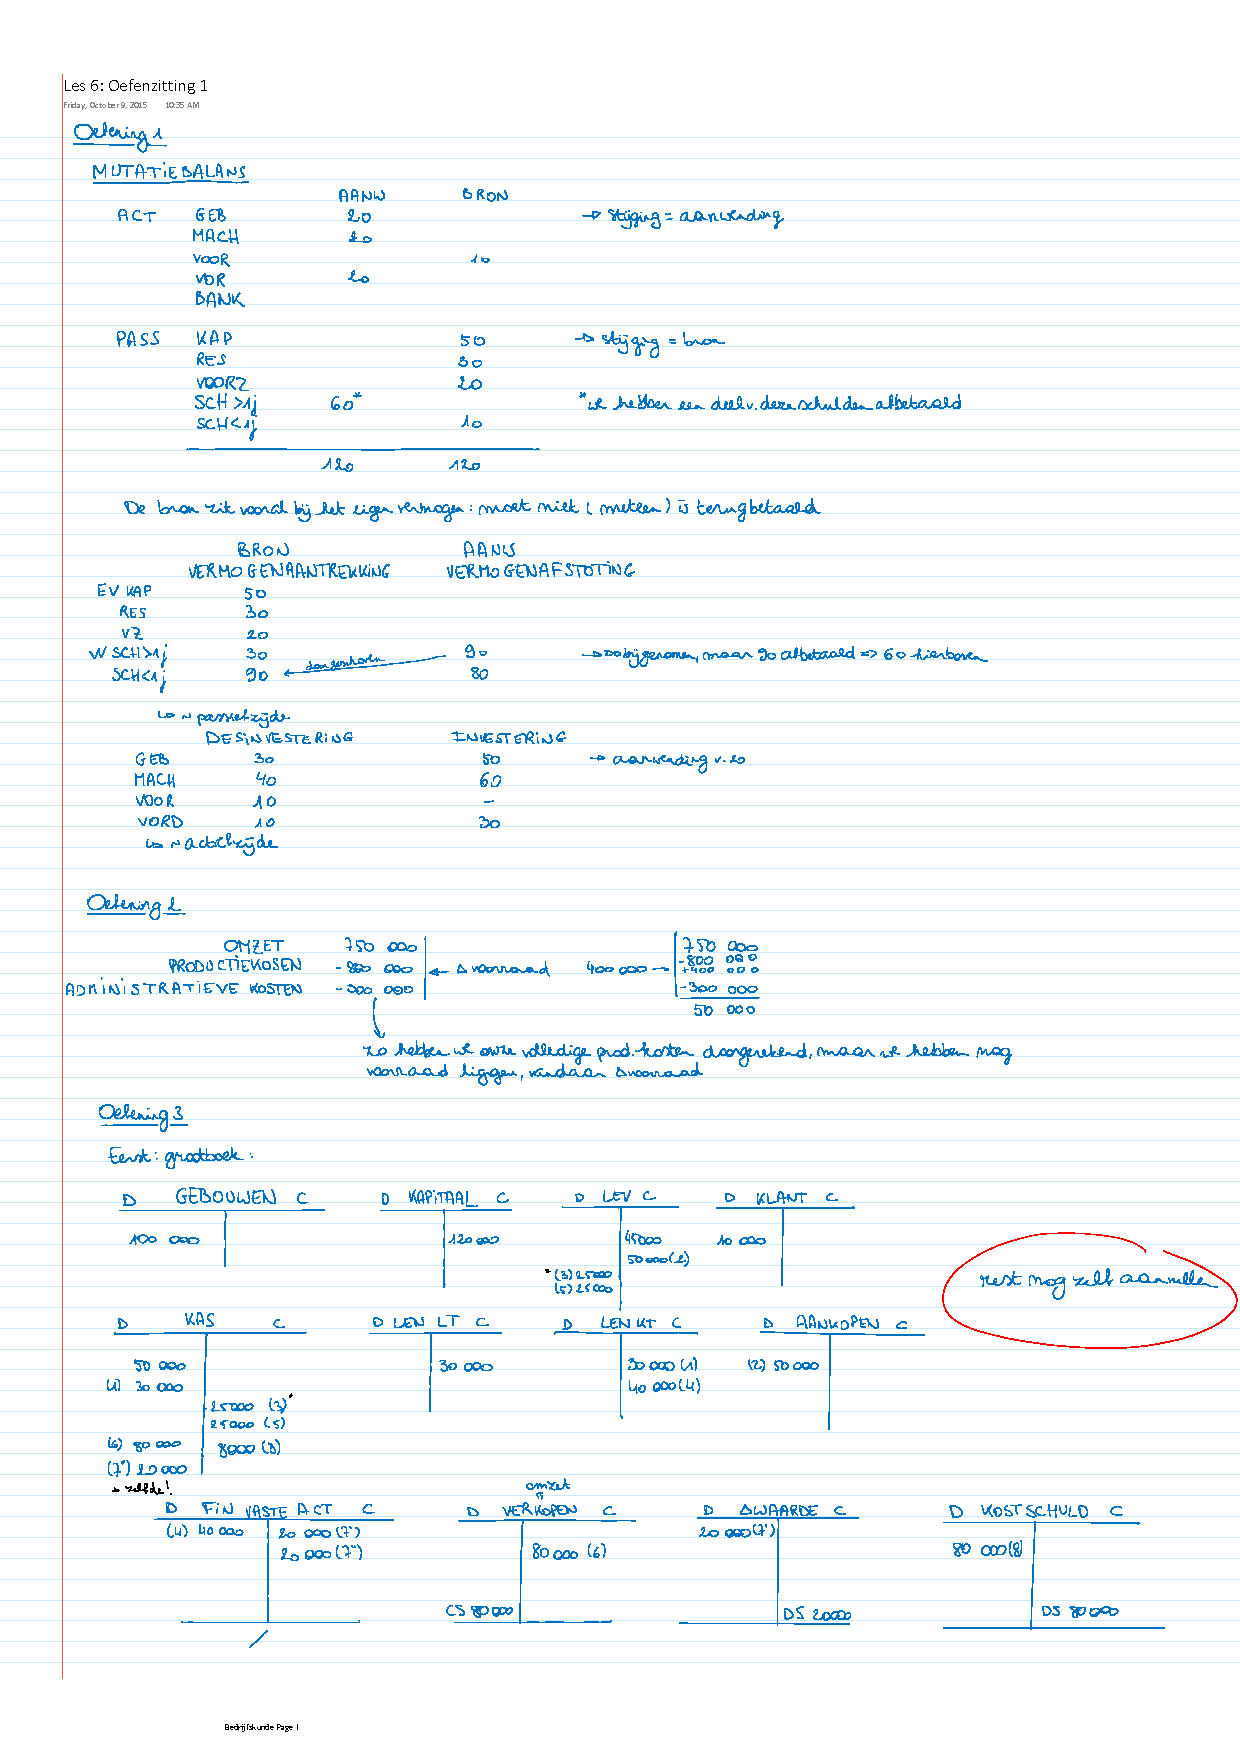
\includepdf[pages={1,2}]{Les6Oefenzitting1.pdf} 

\chapter{Les 7}

\section{Slides: 6\_Bedrijfskunde\_Kostprijssystemen}

\paragraph{Slide 31:} Je kan de kostprijs previsioneel gaan berekenen, maar dan ga je voorspellingen maken. Industri\"ele en evenredige kostprijzen worden berekend voor de toekomst: je moet schattingen maken van lonen, materialen,… en daar zal meestal een afwijking op zitten. Daarom gaaan we ook kijken naar afwijkingsanalyse. \\
Elke keer als iets afgelopen is, moet je kijken waar iets foutgelopen is als er iets fout gegaan is.

\paragraph{Slide 50:} Standaardkosten: zeer vereenvoudigd concept. We hebben de schatting en de werkelijke kost. Deze zullen zeer waarschijnlijk verschillen. We gaan het verschil uitsplitsen in de afwijking: we tellen \'e\'en keer op en trekken \'e\'en keer de elementen van elkaar af. We kunnen zo zien dat er 2 verschillen zijn: verkeerde schatting van het gebruik en verkeerde schatting van de prijs. Als dit groter is dan nul, was de werkelijke kost hoger dan geraamd. De prijsafwijking is $(p'-p)*q$, de effici\"entie-afwijking is $p(q'-q)$.

\paragraph{Slide 51:} Normale productie: de prijs die men verwachtte.

\paragraph{Slide 52 $\&$ 53:} Er zijn 150 000 stuks geproduceerd in plaats van 140 000. Het kostprijsverschil was 40. We hadden een kost van 6 000 000 geschat, maar we hadden een werkelijke kost van 6 140 000. De vraag is nu waar dat verschil vandaan komt. We gaan de formules van \textbf{Slide 51} hierop toepassen: zie Figuur \ref{les07_01}.

\begin{figure}[h!]
\centering
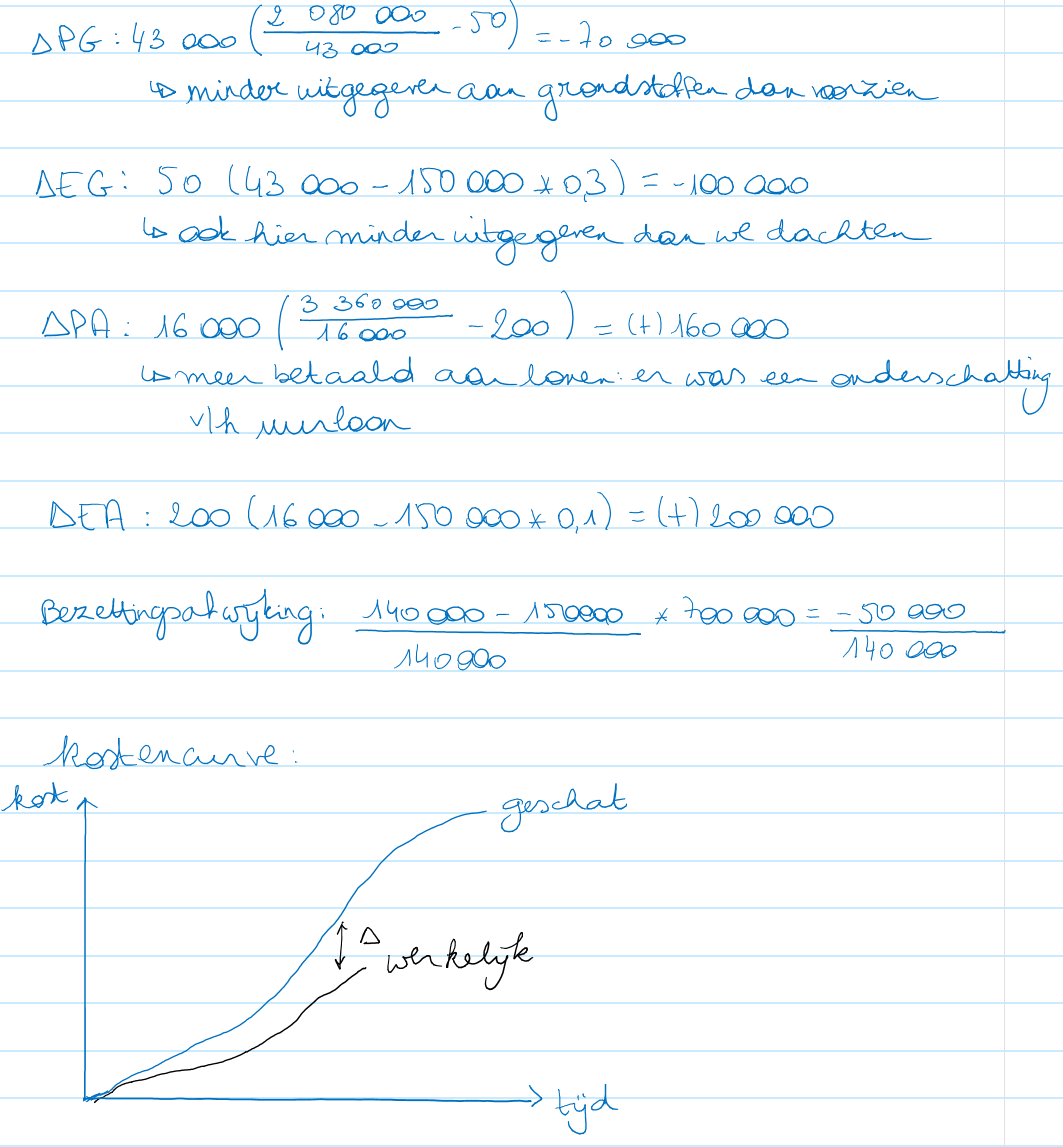
\includegraphics[width=90mm]{Les07_01.png}
\caption{Les 7 Slide 52} 
\label{les07_01}
\end{figure}

\paragraph{Slide 55:} Men besteedt meer aandacht aan overheadkosten.

\paragraph{Slide 56 e.v.:} Als we kijken naar directe arbeid: 400 000 uur per jaar en 1000 wordt gebruikt door A, dus 62 500 wordt toegewezen aan A. Er is niet nagekeken wat er met product A gebeurt. Daarom bekijjken we hetzelfde probleem opnieuw, maar we kijken wat er met A gebeurt in het magazijn.

\paragraph{Slide 58 $\&$ 59:} We delen de kost door de allocatie van de eenheid en krijgen zo de eenheidskost. Het product blijkt arbeidsintensief (de kost/eenheid is 143,75 in plaats van 62,5).

\paragraph{Slide 60:} TD-ABC: Time-Driven Activity Based Costing: men gaat kijken naar alle activiteiten en daar de tijden van noteren: elke actie wordt genoteerd als tijdsspendering aan een bepaalde actie.

\paragraph{Slide 61:} De kostenstructuur is enorm gewijzigd: vroeger waren er 95\% arbeidskosten en 5\% vaste kosten, nu is dat helemaal veranderd. Het grootste probleem is het toewijzen van overheadkosten.\\
Doordat men alle activiteiten gaat analyseren, gaat men een proces opnieuw bekijken en gaat men een aantal activiteiten volledig wijzigen.

\paragraph{Slide 63:} Target costing: reductie van de kosten door een marktonderzoek (nagaan of klanten ge\"interesseerd zijn in het product) en kijken naar de geplande verkoopprijs. We gaan hierbij kijken wat de markt bereid is te betalen voor het product. Daarna kijken we hoe we dat product kunnen opzetten (geld nodig voor materiaal, productie, distributie, levering,…). Dan zorgen dat je aan uw target kosten geraakt (verkoopprijs). Als je bepaalde zaken uitbesteedt, zorg je hierbij soms dat dit onder de target prijs gebeurt (zou moeten).\\
We zijn bezig geweest met kostprijsberekeningen waarbij we aannamen dat alles geproduceerd kon worden. In werkelijkheid gaan er bottlenecks zijn waardoor we niet alles gaan kunnen produceren en we dus een assortiment kunnen bepalen. 

\section{Slides: 7\_Economisch model}

\paragraph{Slide 3:} Wat zullen we maken en waarom?

\paragraph{Slide 4:} We willen de doelfunctie maximaliseren. In dit geval is dat het bedrijfsresultaat (R). We zullen productiehoeveelheden hebben ($q_{i}$) - de kostprijs van de verschillende producten en min de vaste kost (K).\\
We gaan capaciteitsbeperkingen krijgen, ook marktbeperkingen (saturatie van de markt).

\paragraph{Slide 5:} We hebben een doelfunctie met variabelen, kosten en opbrengsten en uiteindelijk hebben we beperkingen op machines, voorraden, beschikbare mensen,… $\rightarrow$ restricties van het aantal stuks/product.

\paragraph{Slide 6:} We kunnen relatief veel commerci\"ele gegevens bepalen. Nadelen: vrij veel variabelen en soms moeten er vereenvoudigingen gedaan worden.

\paragraph{Slide 7 e.v.:} Voorbeeld: Wat gaan we zaaien? Ma\"is of tarwe of een mengeling? Niet alleen kijken naar de opbrengst/ha, maar ook naar de opbrengst/arb. Eerst bepalen wat we als variabele gaan gebruiken. Bv Ton: $T_{t}$ $\&$ $T_{m}$: zie Figuur \ref{les07_02}.

\begin{figure}[h!]
\centering
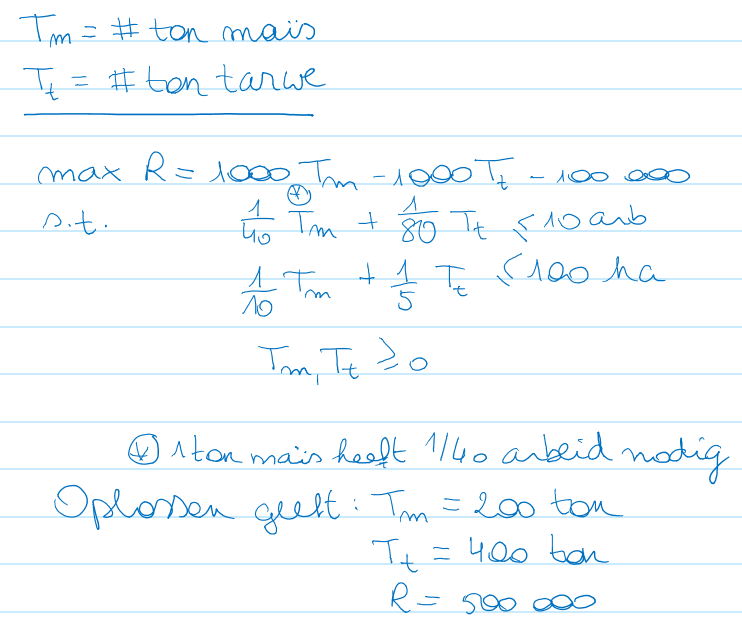
\includegraphics[width=90mm]{Les07_02.png}
\caption{Les 7 Slide 7} 
\label{les07_02}
\end{figure}

We gaan kijken naar de grafische voorstelling op \textbf{Slide 8:} beperkingen in verband met de oppervlakte en de arbeid. De ISO-margelijn is onze doelfunctie. We kunnen die doortrekken tot we in A komen, waarbij we 200 ton ma\"is krijgen en 400 ton tarwe.\\ Interessant is om te weten dat wanneer er een arbeider bijkomt, of dit interessant is of niet en wat het loon is dat eraan gegeven mag worden om geen verlies te maken. We kunnen dit berekenen door de bovenste arbeiderlijn te nemen (arbeider erbij), dan is de oplossing in B. Laten we een arbeider gaan, komen we in C terecht.\\
We kunnen ook kijken naar het duale probleem: als je je bedrijf verhuurt/verkoopt aan iemand anders, wil je minstens uw 500 000 winst terug. We krijgen: zie Figuur \ref{les07_03}.

\begin{figure}[h!]
\centering
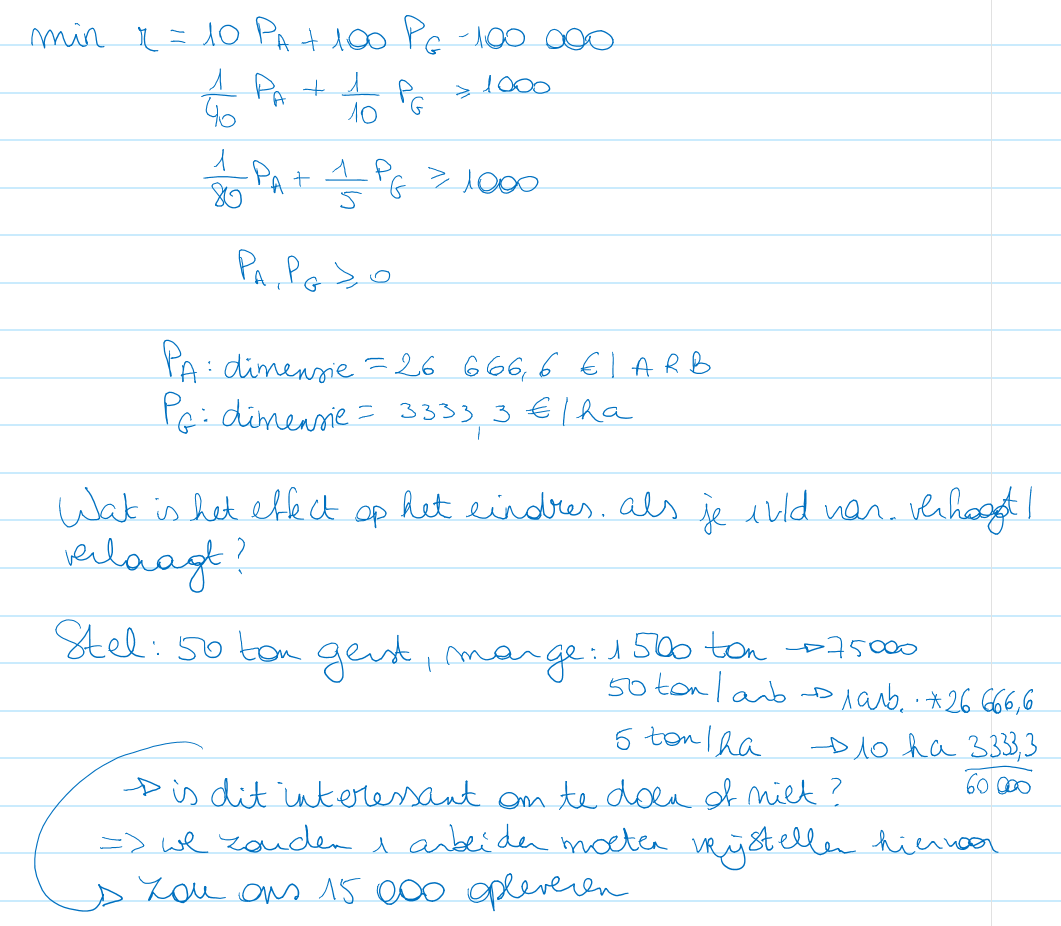
\includegraphics[width=90mm]{Les07_03.png}
\caption{Les 7 Slide 8} 
\label{les07_03}
\end{figure}

\paragraph{Slide 11:} We hebben een bedrijf dat een papiermachine heeft met een beperkte capaciteit van 1000 ton en een kost van 9/kg. Daar worden rollen geproduceerd en we hebben 2 mogelijkheden: ofwel vellen (die worden verpakt), wat ons 2/kg kost, of we pakken de rollen rechtstreeks in, met een extra kost van 1/kg. Deze worden verkocht (D) en daar hebben we verschillende markten: binnenlandse markt $\&$ export voor de vellen en binnenlandse markt $\&$ export voor de rollen. Op basis van wat hier staat kan je bepalen wat de marge per verkoopsas is. De marges staan helemaal onderaan. Je gaat zoveel mogelijk proberen zenden naar de markt met de meeste marge (dus vellen naar het binnenland). Vlak boven de marge staat het optimaal verkoopprogramma. Die 500 komt van bij het beentje van binnenland, de 200 = 700 (bij B) - 500, hierbij is dan al 700 toegewezen en voor rollen binnenland is 100 optimaal, we hebben dan nog 200 over die naar de export van rollen gaat.\\
Als we kijken naar de schaduwkosten: zie Figuur \ref{les07_04}.

\begin{figure}[h!]
\centering
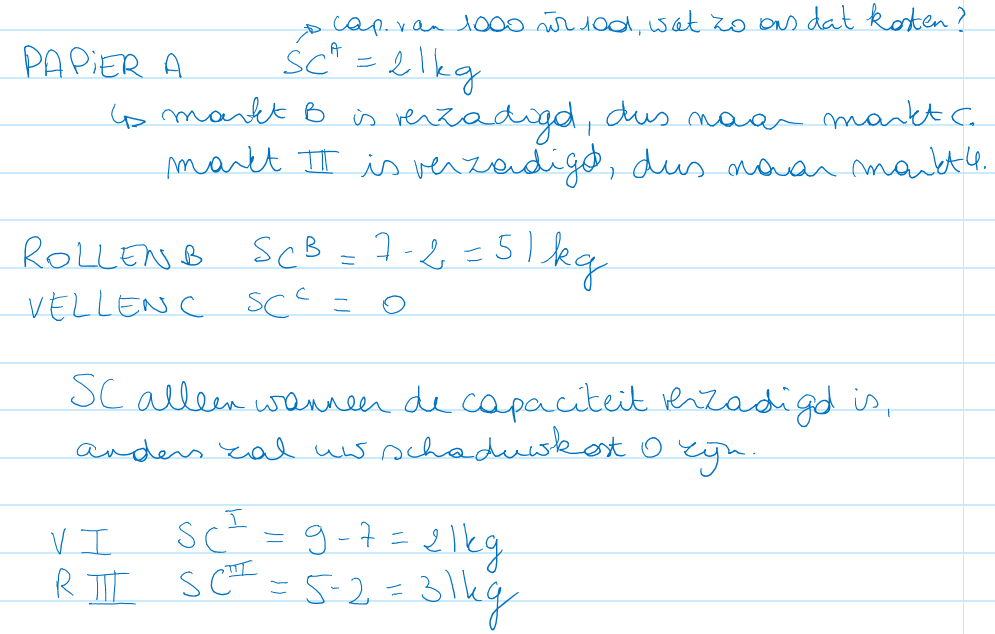
\includegraphics[width=90mm]{Les07_04.png}
\caption{Les 7 Slide 11} 
\label{les07_04}
\end{figure}

\paragraph{Slide 10:} Stel dat we een rol (\textbf{Slide 11}) willen verkopen/aankopen: welke prijs moet je daarvoor vragen? Doordat je die ene rol eruit haalt, zal je 999 rollen produceren en zal je 2 verliezen. Maar ook het inpakken van de rollen moet je inrekenen. De transferprijs is dus 9+1+2 = 12/kg. Als je de rollen verkoopt aan iemand, vraag je minstens 12, als je er een aankoopt, betaal je minstens 12.\\
Kijken we naar de transferprijs onder A (die grote pijl), dan krijgen we de schaduwkost van machine A, maar hij gaat niet meer door het inpakproces, dus we krijgen: 9+2 = 11/kg. We willen dat onze totaalverkoop qua prijs dezelfde blijft.

\paragraph{Slide 13:} Op het eerste zicht is P1 interessanter dan P2 (want 1000/stuk), maar je hebt voor P1 2 uur nodig en voor P2 maar 1 uur, wat dus neerkomt op een totaal van 500 voor P1 en 800 voor P2. P2 is dus interessanter. Als we dit in een figuur steken, krijgen we: zie Figuur \ref{les07_05}.

\begin{figure}[h!]
\centering
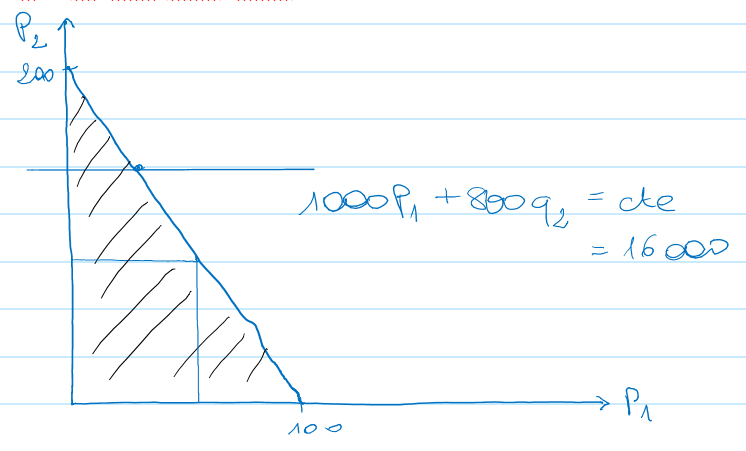
\includegraphics[width=90mm]{Les07_05.png}
\caption{Les 7 Slide 13} 
\label{les07_05}
\end{figure}

\paragraph{Slide 15:} Ander voorbeeld.\\
Conclusie: Je moet alles gaan bekijken. Als je alles kunt produceren, ga je vooral kijken naar de minimalisatie van kosten. Als je een bottleneck hebt, kun je niet alles produceren en moet je gaan uitzoeken wat voor jou het meest interessante is. Dan ga je kijken naar de marge/uur kosten. 

\chapter{Les 8}

\section{Slides: 8\_Bedrijfskunde\_Budgettering en kasplanning}

\paragraph{Slide 1:} Bedrijven moeten altijd een plan met budgetten voor de komende 5 jaar voorleggen om aan te tonen dat ze kunnen blijven bestaan, dat ze voldoende cash flow zullen kunnen genereren om te kunnen blijven bestaan.

\paragraph{Slide 3:} Elk bedrijf gaat een strategische planningscyclus hebben waarbij men bv. werkt met een tijdshorizon van 5 jaar waarbij men alle kosten zal vastleggen en ieder jaar schuift men een jaar verder door. Op het eind van het jaar gaat men analyseren wat er eventueel anders gelopen is dan voorzien en waarom.\\
Je gaat dus iedere keer een raming maken van inkomsten en uitgaven. 
Je gaat van alles inkomsten en uitgaven proberen te schatten en dit achteraf bekijken. Je moet dus kijken naar de liquiditeit en solvabiliteit (``Kunnen we de leningen, lonen,… betalen?").

\paragraph{Slide 5:} Je moet kunnen plannen en de zaken kaderen binnen de doelstellingen van het bedrijf. Je moet gaan organiseren (kan gekoppeld zijn aan de producten of aan de markten), mensen gaan motiveren en achteraf zelf controleren  en nagaan hoe alle middelen zijn toegepast.

\paragraph{Slide 6:} Gewone begroting: elk jaar een budget opstellen voor de komende 5 jaar. Investeringsbudgetten zijn eerder buitengewone begrotingen. 

\paragraph{Slide 7:} Dit is wat we willen weten: wat is onze winst, wat is onze opbrengst en wat zijn onze kosten? Het is niet zeker dat dit het eindresultaat zal zijn, vandaar dus ``(geplande)".\\
Voorraden: het opstapelen van voorraden kost ook geld, dat zit vast in uw magazijn en dat geld kan je niet gaan investeren in iets anders.

\paragraph{Slide 9:} Zie Figuur \ref{les08_01}.

\begin{figure}[h!]
\centering
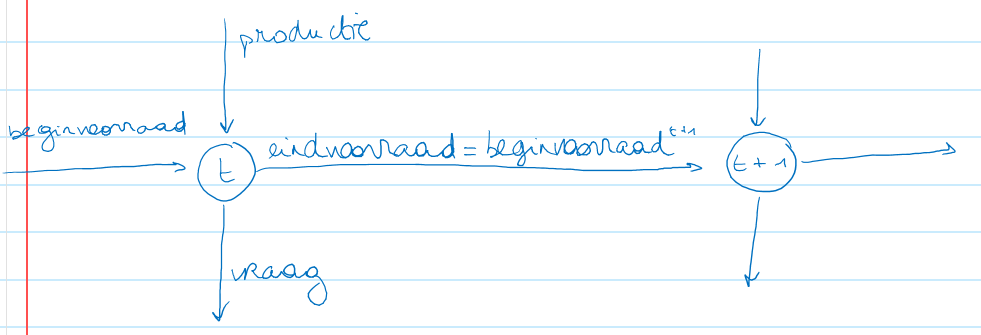
\includegraphics[width=90mm]{Les08_01.png}
\caption{Les 8 Slide 9} 
\label{les08_01}
\end{figure}

\begin{itemize}
\item Seizoenmatigheid: soms heb je pieken in de verkoop.
\item Bederfbaarheid: voorraadrotatie zo maken dat uw producten buiten zijn voor ze bedorven zijn.
\item Voorraadkosten: sommige producten moeten op speciale manieren bewaard worden (gekoeld, verwarmd,…).
\item Aankoopbeleid: kunnen we bepaalde batches aankopen en hoe groot moeten/mogen die dan zijn?
\end{itemize}

\paragraph{Slide 10:} Investeringsbudget: als je merkt dat uw capaciteit onvoldoende is om aan de vraag te voldoen, moet je investeren in nieuwe machines/mensen/… 

\paragraph{Slide 11:} Het is nodig te weten wanneer er tekorten/overschotten zijn, of sommige zaken verschoven kunnen worden, welke leningen aangegaan kunnen worden,… $\rightarrow$ previsionele resultatenrekening en balans.

\paragraph{Slide 13:} Voorbeeld: de meeste van die getallen zijn daar gewoon geplaatst (probeer ze dus niet zelf te berekenen!). Er worden soms ook afrondingen gemaakt, dus geen exacte berekeningen. Het is de bedoeling dat we proberen om zo'n tabel op te stellen. 

\paragraph{Slide 14:} Bedrijf verkoopt product X $\&$ Y, met 3 markten. Via marketingstudies checken we wat de verkopen zouden kunnen zijn in het volgende jaar (dus enkel 1 jaar bekijken, geen reeks jaren). De verkoopsaantallen zijn te zien in de onderste rij an de tabel (in kolommen van ``Eenheden"). 210 000 * 100 = 21 000 (* $10^{3}$, zie bovenaan). We gaan kijken hoe het zit met onze voorraaden. Dit zien we in de Begininventaris van de tweede tabel. Je ziet dat je niet 1 000 000 stuks gaat produceren, maar 960 000. Dit is afhankelijk van de situatie (o.a. waar in de cyclus je zit).

\paragraph{Slide 15:} Op basis daarvan kunnen we zien wat de voorraadwaarde is en de waarde per stuk (168 en 69). Een product is meestal samengesteld uit deelproducten. We gaan nog MRP (Material Requirement Planning) zien. Product X wordt samengesteld uit A, B en C: dit is de productstructuur (zie tekening op Figuur \ref{les08_02}).

\begin{figure}[h!]
\centering
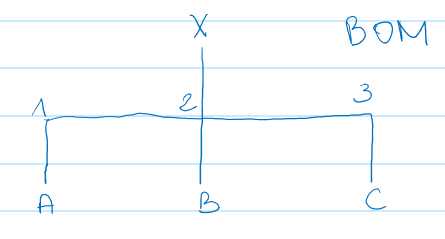
\includegraphics[width=60mm]{Les08_02.png}
\caption{Les 8 Slide 15} 
\label{les08_02}
\end{figure}

\paragraph{Slide 16:} Op basis van de voorgaande berekeningen kunnen we gaan zien hoeveel stuks we moeten gaan produceren.\\
We zien hoeveel stuks van A, B en C we nodig hebben. Hier krijgen we dan de brutobehoeften van de verschillende grondstoffen. 

\paragraph{Slide 17:} Rekening houdend met de beginvoorraad en de gewenste eindvoorraad krijg je de tabel. 

\paragraph{Slide 18:} Directe loonkosten de gelinkt zijn aan de productie. 

\paragraph{Slide 19:} Indirecte kosten: de cijfers zijn ter illustratie, niet ergens berekend. Wij zijn ge\"interesseerd in de 39 939 onderaan.

\paragraph{Slide 20:} De kostprijs die we mogen aanrekenen is kleiner dan onze aankoopprijs (70 830 000 vs 70 950 000), dit komt omdat we met voorraden zitten, we mogen die niet zomaar doorrekenen.

\paragraph{Slide 23:} Alles samenbrengen: previsionele resultatenrekening. 

\paragraph{Slide 24:} Uiteindelijk zal het zo zijn, op basis van onze productie en het feit dat het productiepark veroudert, dat we een investeringsbudget moeten samenstellen. Sommige zaken zullen over verschillende jaren lopen, je moet dat proberen opsplitsen. 

\paragraph{Slide 27:} Een budget moet opgesteld worden en je moet dit achteraf gaan controleren op verschillende facetten. Je moet ervoor zorgen dat iedereen op de hoogte is van de budgetten. Het is niet omdat iemand iets aanvraagt, dat hij/zij dat budget ook altijd krijgt, die moet zijn/haar budget eventueel ook gaan aanpassen aan wat toegewezen wordt. 

\paragraph{Slide 29:} Interpretatie van een aantal zaken.

\paragraph{Slide 30:} We gaan kijken naar de afwijking van het gebudgetteerde bedrag en de werkelijkheid. Je gebruikt bij de werkelijke productie ook 1875 omdat dat het aantal is dat je werkelijk geproduceerd hebt, maar je moet wel gaan kijken naar uw voorspelde waarden (standaard materiaalverbruik en gebudgetteerde materiaalprijs). Het materiaalverbruik en de materiaalkost bleek hoger dan voorspeld. 

\paragraph{Slide 32:} 180 000 komt van 1875 * 96. 196 875 komt van 1875 * 105. Als we effici\"ent waren geweest, had het prijsverschil even breed geweest als ``budget bij standaardverbruik", maar nu is dat dus ``budget bij standaardverbruik" + ``effici\"entieverschil).

\paragraph{Slide 33:} Zie Figuur \ref{les08_03}.

\begin{figure}[h!]
\centering
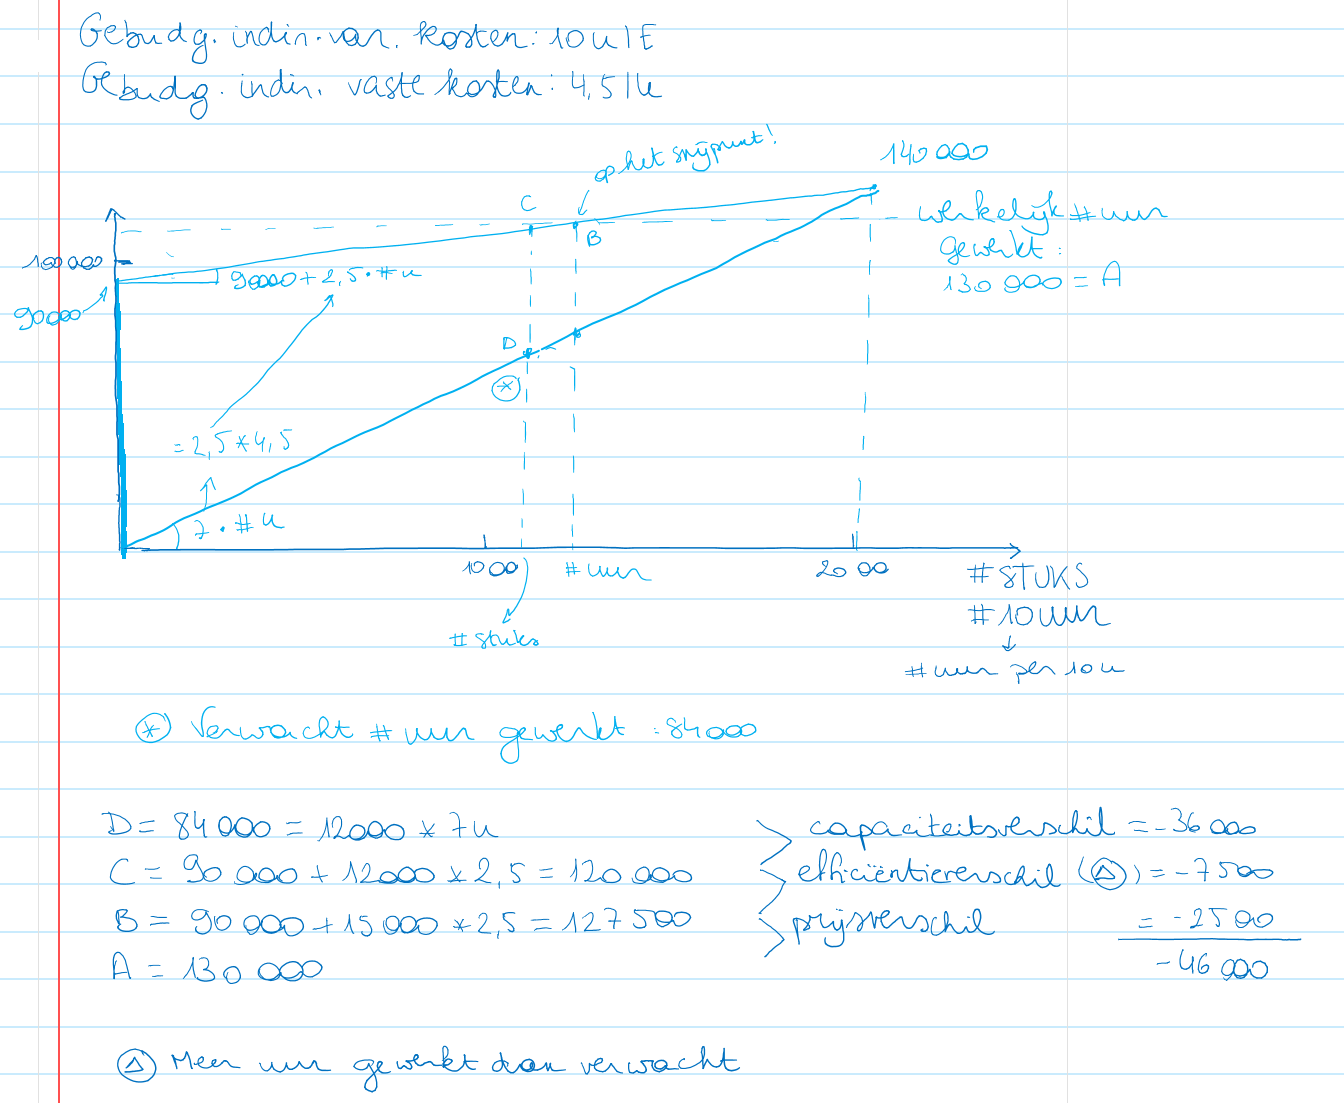
\includegraphics[width=120mm]{Les08_03.png}
\caption{Les 8 Slide 33} 
\label{les08_03}
\end{figure}

\paragraph{Slide 34:} Berekeningen bij de grafiek. Het effici\"entieverschil is puur afkomstig van variabele kosten (denk ik).
    
\section{Slides: 9\_Bedrijfskunde\_Investerings- en kostenbatenanalyse}

\paragraph{Slide 3:} Als we investeren in een nieuwe productie-eenheid (bv. fabriek), moeten we gaan nagaan waar het interessant is om te gaan investeren. 

\paragraph{Slide 4:} Het basisprincipe van een investering: we hebben een investering waarbij we een bepaald bedrag uitgeven op een bepaald tijdstip en we hopen achteraf dat we geld extra zullen binnenkrijgen. Dat geld komt dan over een bepaalde tijdsperiode binnen, afhankelijk van de duur van onze investering. Op die manier genereer je bepaalde kasstromen. Je moet zorgen dat uw binnenkomend geld voldoende groot is om uw investering te compenseren.

\paragraph{Slide 5:}
\begin{itemize} 
\item Vervangingsprobleem: het systeem is fysisch verouderd (werkt bv. niet meer). 
\item Moderniseringsprobleem: machine kan niet meer mee.
\item Strategisch probleem: meestal wanneer je een nieuw product op de markt brengt en de markt groeit of met dalende marktvraag omgaan.
\item Expansieprobleem: nieuwe eenheden plaatsen op nieuwe locaties.
\end{itemize}

\paragraph{Slide 6:}
\begin{itemize}
\item Fysische levensduur: verouderde machines.
\item Economische levensduur: als uw product goedkoper gemaakt kan worden.
\item Productlevensduur: als uw product na 3 jaar verouderd is, ga je niet voor 10 jaar investeren in dat product, maar maar voor 3 jaar.
\item Fiscale levensduur: afschrijvingen.
\end{itemize}
Als je projecten gaat vergelijken met elkaar, moeten dat gelijkwaardige projecten zijn (project dat 2 jaar duur vs een project dat 5 jaar duurt). \\
Uitgavepatroon: alle investeringsonkosten moeten daarin gerekend worden. Je moet kijken naar alle kosten zodanig dat uw installatie kan werken.

\paragraph{Slide 7:} Kasstroom: inkomsten en uitgaven per periode (kunnen vari\"eren per periode), we krijgen dan de bruto kasstroom. Daarvan gaan we de afschrijvingen aftrekken, zo krijgen we de belastbare winst waarvan we de belastingen moeten betalen, waarop we de winst na belastingen krijgen. Daarna tellen we er de afschrijvingen opnieuw bij op (soort recuperatie die je mag doen door minder belastingen te betalen. Je moet die afschrijvingen niet nog eens betalen want dan zou je 2 keer betalen). \textcolor{red}{Als je afschrijvingen ziet als kasstromen op het examen, ben je gebuisd voor die vraag.}

\paragraph{Slide 8:} Het is belangrijk om de juiste kosten te kennen. Kern van de zaak is dat je alles wilt omzetten in geld.

\paragraph{Slide 9:}
\begin{itemize}
\item Samengestelde interesten: veronderstel dat we ergens een bepaald kapitaal p hebben dat we beleggen. Als we dat beleggen aan een bepaalde interest, wil dat zeggen dat na 1 periode het kapitaal gelijk is aan P + Pi. Als je dat bedrag dan opnieuw belegt, dan zal P vermenigvuldigd worden met i, maar uw interest ook. Het kapitaal waarmee we startten zal dus gelijk zijn aan $F = P(1+i)^{n}$ als je alles hebt laten staan.
\end{itemize}
\paragraph{Slide 10:} Bij hoge interestvoeten zie je dat je niet lineair mag denken, bij kleine interestvoeten zal de geschatte en de werkelijke opbrengst ongeveer gelijklopen.

\paragraph{Slide 11:} De meest linkse kolom is het aantal periodes. Bovenaan vind je dan telkens het aantal percentages terug. Je ziet dan na hoeveel periodes je hoeveel zal hebben.

\paragraph{Slide 13:} We gaan normaal alles proberen terugbrengen naar het ``nu"-moment: naar de waarden die nu geldig zijn. Daarom spreken we over actualisatie. 

\paragraph{Slide 15 $\&$ 16:} Huidige waarde van 1 Euro. Let op dat er gesproken is over periodes en niet over jaren. Het kan zijn dat men over trimesters spreekt en niet over jaren.

\paragraph{Slide 17:} We zullen niet 1 bedrag hebben dat binnenkomt, maar dat zal verspreid zijn over de horizon. Dit kunnen uiteraard ook negatieve waarden zijn. Je moet uiteindelijk altijd vergelijken met het nulmoment.

\paragraph{Slide 18:} We kunnen de gegeven vraag gaan berekenen: zie Figuur \ref{les08_04}.

\begin{figure}[h!]
\centering
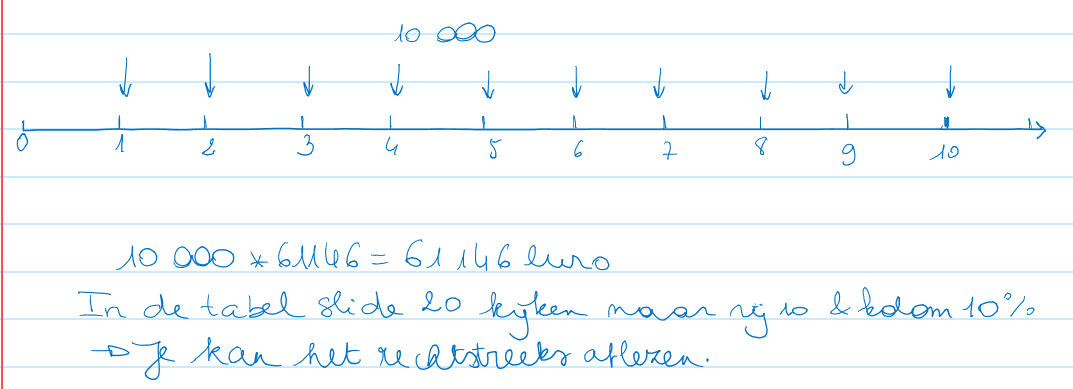
\includegraphics[width=90mm]{Les08_04.png}
\caption{Les 8 Slide 18} 
\label{les08_04}
\end{figure}

\paragraph{Slide 21:} Banklening van 100 000 en je hebt een trimesteri\"ele rentevoet van 4\%. De terugbetalingen gebeuren altijd op een specifiek moment. We hebben n = 5 en I = 4\%. Kijken we in onze tabel op \textbf{Slide 19} (rij 5, kolom van 4\%), krijgen we: A*4,4518 = 100 000 $\Rightarrow$ A = 22 463.\\
Hoe wordt dat nu allemaal uitgesplitst? Zie Figuur \ref{les08_05}.

\begin{figure}[h!]
\centering
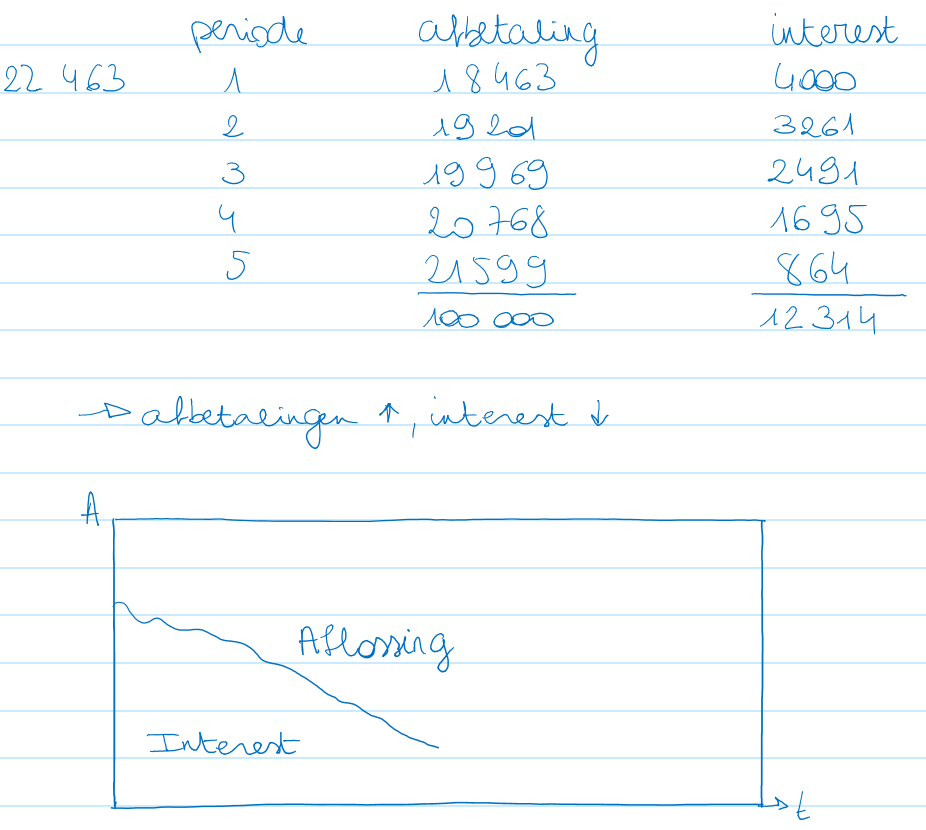
\includegraphics[width=90mm]{Les08_05.png}
\caption{Les 8 Slide 21} 
\label{les08_05}
\end{figure}

\paragraph{Slide 22:} Overgeslagen.

\paragraph{Slide 23:} Zie Figuur \ref{les08_06}.

\begin{figure}[h!]
\centering
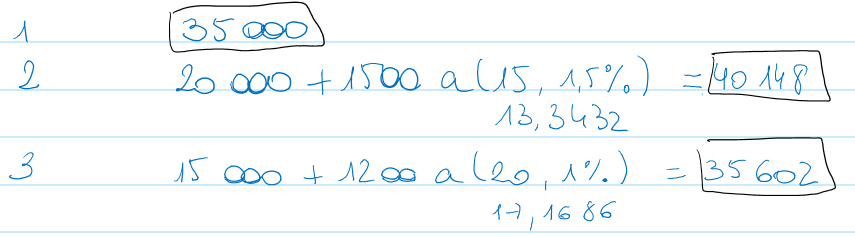
\includegraphics[width=90mm]{Les08_06.png}
\caption{Les 8 Slide 23} 
\label{les08_06}
\end{figure}

Niet zomaar voor 2 of 3 kiezen, je moet nog steeds 20 000 investeren! De eerste optie is duidelijk de goedkoopste.

\chapter{Les 9}

\section{Slides: 9\_Bedrijfskunde\_Investerings- en kostenbatenanalyse}

\paragraph{Slide 24:} We weten hoe snel een investering wordt terugbetaald. Op de horizontale as hebben we de tijdshorizon, op de verticale as hebben we een overzicht van de kasstromen. Op tijdstip 0 hebben we ons investeringsbedrag gehad. Het is de bedoeling dat zo'n investering geld opbrengt in de toekomst. Wanneer we alles cumulatief uitzetten, is het de bedoeling dat de positieve kasstromen groter worden dan de negatieve zodat we boven 0 uitkomen, anders is de investering niet interessant. Bij curve 1 komen we relatief snel naar boven en hebben we een relatief korte terugbetalingstermijn. Bij de tweede is dat minder snel. Het eerste project is dus interessanter dan het tweede. Dit heeft een aantal nadelen: we zijn kortzichtig want we kijken alleen naar de eerste inkomsten en niet naar latere inkomensten, we willen ons geld zo snel mogelijk opnieuw recupereren. We houden geen rekening met achterliggende inkomsten.\\
Curve 2 toont mooie kasstromen later, maar je kan de verre toekomst niet voorspellen. In de nabije toekomst kan je veel beter voorspeleln. Daarom kijkt men voornamelijk naar hoe snel de investering wordt terugbetaald.

\paragraph{Slide 25:} Men gaat kijken naar de netto waarde. We kijken naar de kasstroom teruggebracht naar het nu-moment. We gaan kijken naar de inkomsten (R: revenue) en uitgaven (E: expenses). Daar nemen we de netto waarde van en passen we die aan met de juiste actualisatievoet om die terug te brengen naar het nu-moment. Naarmate k stijgt, wordt de factor in de noemer groter en gaat de waarde dalen in het nu-moment.\\
Meestal kijkt men naar de netto huidige waarde: huidige waarde - investeringsbedrag. Een investering is interessant wanneer de netto huidige waarde positief is. Als we moeten kiezen tussen 2 projecten, kiezen we dat project met de grootste netto huidige waarde. NHW(A) = 10 000 NHW(B) = 8000. Je zou intu\"itief voor A kiezen, maar je weet hier niets over de tijd. Je moet ook kijken naar het investeringsbedrag: stel: $I_{0A}$ = 1 000 000 en $I_{0B}$ = 250 000. Bij B heb je nog 750 000 over die ook iets zullen opbrengen. Je moet altijd alles dus op de juiste manier analyseren en bekijken.

\paragraph{Slide 26:} Meest gebruikt: houdt rekening met beiden. We hebben gemerkt dat 2 verschillende regels 2 verschillende rangordes kunnen geven. Je moet alles dus altijd grondig analyseren en bekijken.

\paragraph{Slide 27:} Inwendige rendementsgraad: als we ergens onze NHW plaatsen in functie van de interestvoet, dan gaan we die berekenen voor een bepaalde i. hopelijk vinden we dan ergens een positieve waarde. Laten we die i vari\"eren, zal die waarde ook mee vari\"eren. Als we werken met een systeem waarbij we 1 uitgave hebben en voor de rest allemaal inkomsten, wat zal er dan gebeuren als de i kleiner wordt, wat gebeurt er dan met de NHW? Als i kleiner wordt, zal de waarde stijgen. Zie Figuur \ref{les09_01}.

\begin{figure}[h!]
\centering
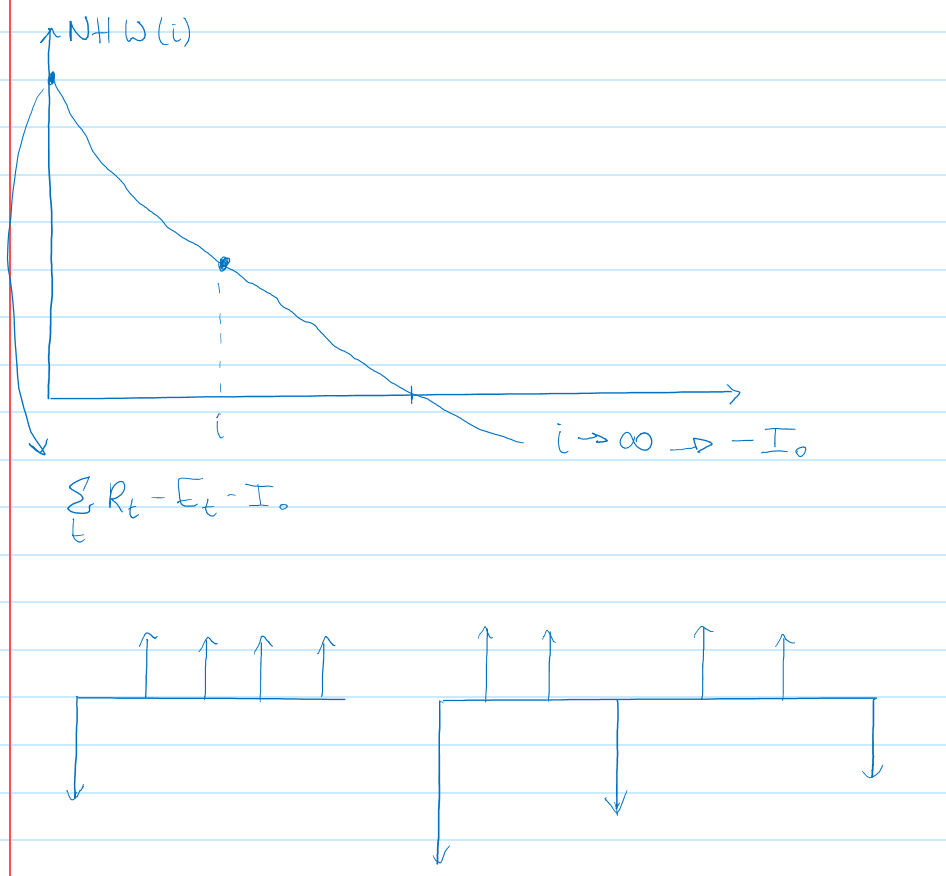
\includegraphics[width=90mm]{Les09_01.png}
\caption{Les 9 Slide 27} 
\label{les09_01}
\end{figure}

\paragraph{Slide 29:} 1 is interessanter (via de inwendige rendementsgraad) dan 2, terwijl we volgens de NHW net het omgekeerde vinden. Je moet dan gaan nagaan hoe het juist zit. 

\paragraph{Slide 30:} Zie Figuur \ref{les09_02}.

\begin{figure}[h!]
\centering
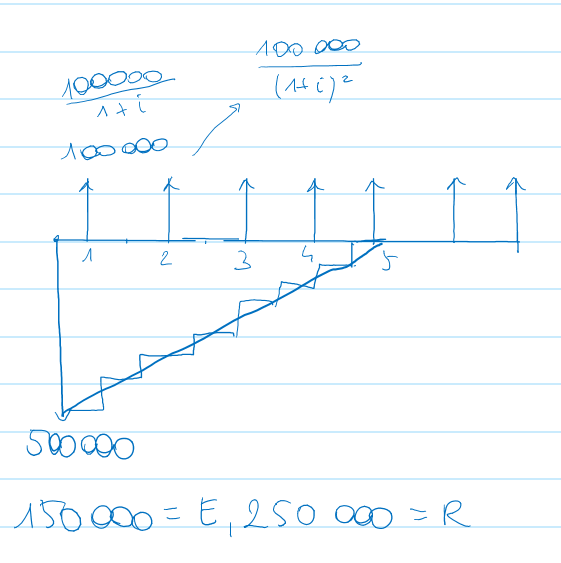
\includegraphics[width=90mm]{Les09_02.png}
\caption{Les 9 Slide 30} 
\label{les09_02}
\end{figure}

\paragraph{Slide 31:} Zie Figuur \ref{les09_03}.

\begin{figure}[h!]
\centering
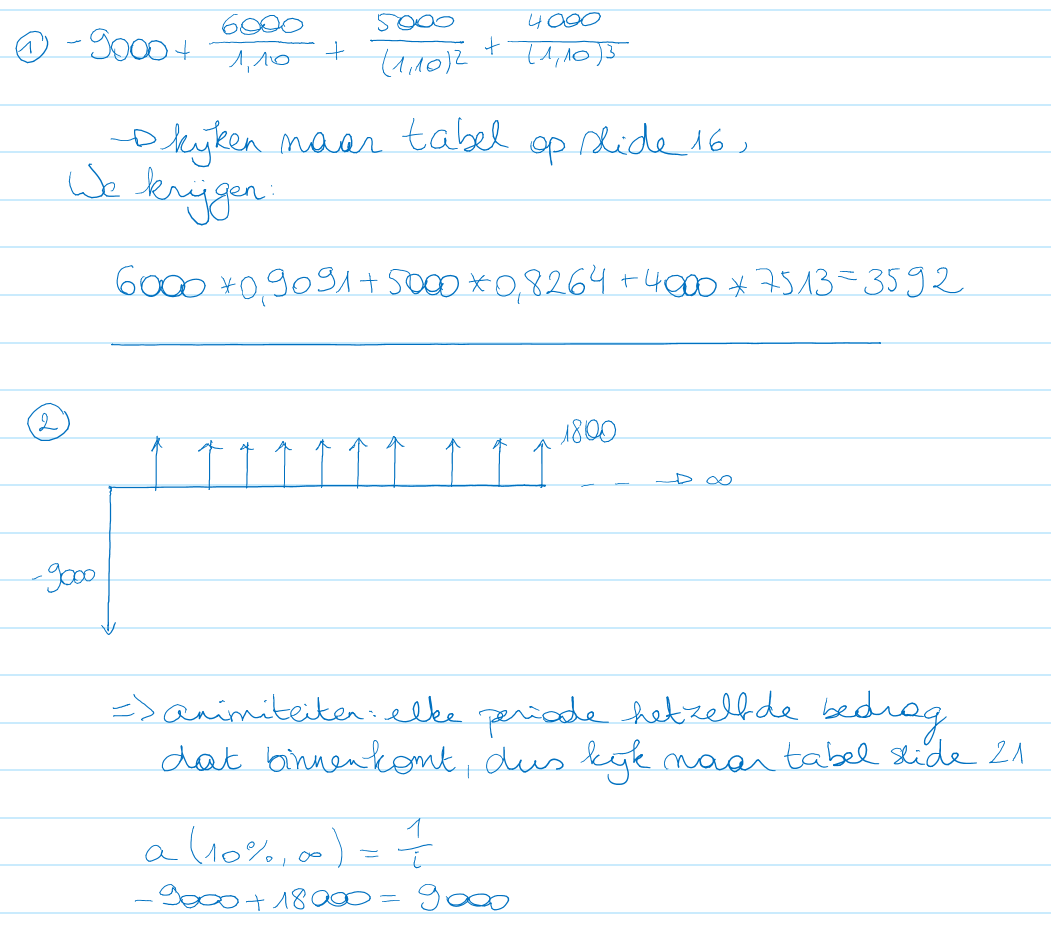
\includegraphics[width=90mm]{Les09_03.png}
\caption{Les 9 Slide 31} 
\label{les09_03}
\end{figure}

\paragraph{Slide 32:} Let op: lichte aanpassingen tegenover het boek. We gaan maar 500 000 afschrijven en geen 600 000. Zie Figuur \ref{les09_04} $\&$ \ref{les09_05}.

\begin{figure}[h!]
\centering
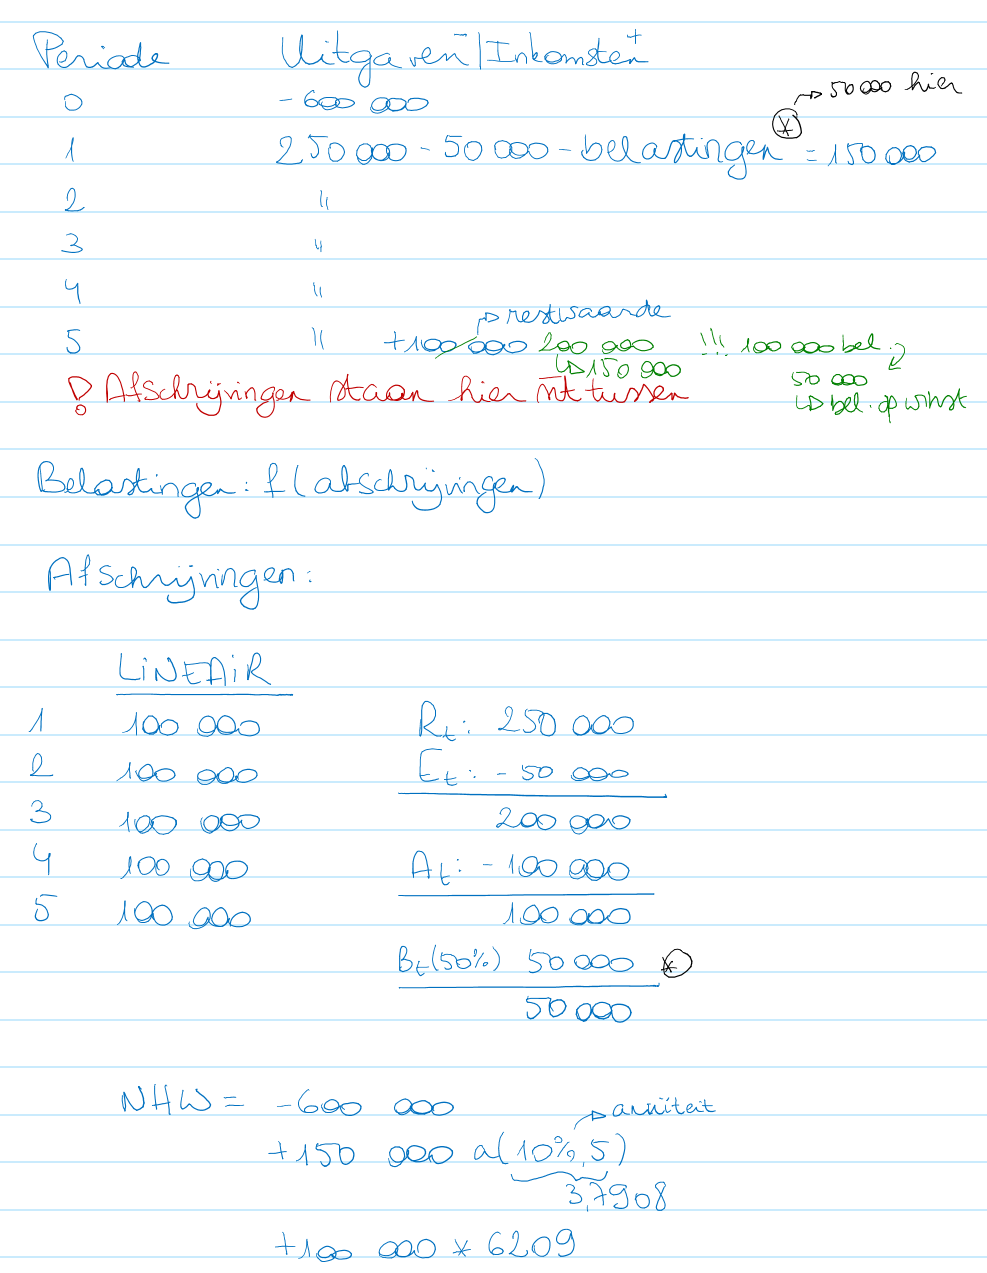
\includegraphics[width=90mm]{Les09_04.png}
\caption{Les 9 Slide 32} 
\label{les09_04}
\end{figure}

\begin{figure}[h!]
\centering
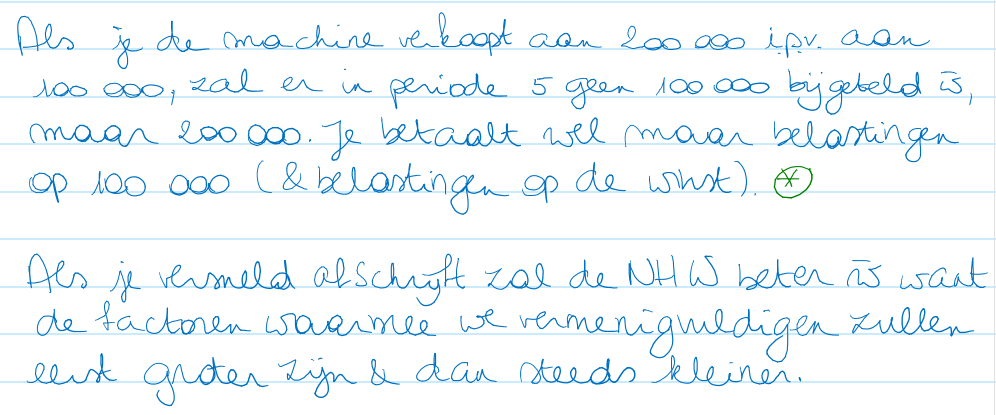
\includegraphics[width=90mm]{Les09_05.png}
\caption{Les 9 Slide 32} 
\label{les09_05}
\end{figure}

\paragraph{Slide 33:} Project z zal het interessantst zijn.

\paragraph{Slide 34:} Hier moet je ook rekening mee houden, kan uw resultaten ook be\"invloeden. Men gaat normaal ook nooit werken met 1 interestvoet, maar met verschillende om te kijken wat de variatie is, want als je curve steiler is, zal een variatie in i een zeer groot effect hebben en wanneer ze minder steil is, zal een variatie in i nauwelijks effect hebben.

\paragraph{Slide 36:} Soort screening: kijken of een project aan een bepaalde eis voldoet. Naarmate de `qualifies' stijgt, zal het project interessanter zijn.

\paragraph{Slide 37:} Een meer genuanceerd antwoord.

\paragraph{Slide 35:} Ook meer uitgebreide technieken.

\paragraph{Slide 38:} De beoordeling van \textbf{Slide 37} visueel voorgesteld. B scoort overal slechter dan A (tenzij gelijk). Je zal dus nooit B nemen als je A kan nemen. Bij C is het genuanceerder, daar hangt het er vanaf aan welk criterium je meer waarde hecht.

\paragraph{Slide 39:} Gradaties en gewichten. Het grote probleem hiermee is dat men elk resultaat kan bekomen wat men wil. Dit mag niet ingevuld worden door 1 persoon, maar door verschillende waarbij duidelijk te zien is wie wat doet.

\section{Slides: 10\_Bedrijfskunde\_Voorspellingstechnieken}

\paragraph{Slide 3:} Hoeveel banden gaan we maken in augustus? Is dit een makkelijke vraag? Bandenbedrijven zullen dit vrij goed kunnen schatten op basis van de verkoop van wagens etc. Normaal heb je eerst een order dat binnenkomt voor de aankoop van wagens en op basis daarvan zullen ze gaan voorspellen hoeveel banden er gemaakt moeten worden.

\paragraph{Slide 5:} We moeten rekening houden met het tijdsschema: afhankelijk van of we op korte of lange termijn voorspellen, gaan we op een ander niveau werken. Werken we op lange termijn, dan gaan we geaggregeerd werken. Bij lange termijn gaat men kijken naar capaciteitsbehoeften, bij intermediate gaat men kijken naar mensen en bij short gaat men kijken naar shifts.

\paragraph{Slide 6:} Voorspellingstechnieken zijn meestal fout: zie ook \textbf{Slide 7}. Als we bezig zijn met voorspellingen, moet je ervoor zorgen dat je niet eender welk getal krijgt, maar ook redenen geven waarom je dingen denkt. Het zou ook neergeschreven moeten zijn zodat men niet zomaar van mening kan veranderen. Geaggregeerde voorspellingen zijn vrij eenvoudig. De eerste jaren die we voorspellen zijn meestal vrij nauwkeurig, daarna wordt het minder nauwkeurig. \\
Je moet ook altijd proberen alle mogelijke informatie te gebruiken die aanwezig is. 

\paragraph{Slide 8:} Een goede forecast moet:
\begin{itemize}
\item op tijd zijn: als je achteraf voorspellingen doet, is het natuurlijk makkelijk;
\item zo nauwkeurig mogelijk zijn;
\item betrouwbaar zijn;
\item betekenisvolle eenheden hebben;
\item opgeschreven zijn;
\item begrijpbaar zijn voor eventuele opvolgers.
\end{itemize}

\paragraph{Slide 9:} Je moet beginnen met het identificeren van het probleem. Je moet voorspellingen doen voor zaken die nuttig en interessant zijn. Je moet zorgen dat je het probleem kent.

\paragraph{Slide 10:} Je moet kijken naar de impact en of het een eenmalige beslissing is, of een beslissing die regelmatig terugkomt. Je moet iets maken dat wel degelijk werkt als het terugkerend is, bij eenmalig kan je eventueel anders werken.

\paragraph{Slide 11:} We gaan kijken of er data beschikbaar is. Als die beschikbaar is, moet je die gaan analyseren. Dit is een heel belangrijke stap. Je moet ook gaan kijken of uw data al dan niet kwantitatief is. Als ze kwantitatief zijn, kan je kijken of er causale factoren zijn (bv. verkoop van wagens $\rightarrow$ verkoop van banden).
Als er geen causale factoren zijn, gaan we tijdsanalyses doen. Als men geen data heeft, gaat men die moeten collecteren. Deze kunnen kwantitatief zijn. Als de gegevens kwalitatief zijn, gaat men ook anders te werk.

\paragraph{Slide 12:} Je moet het probleem snappen, weten wat er gebeurt. Je moet proberen alle mogelijke extra informatie erbij te krijgen. Het is belangrijk dat je begrijpt wat er juist aan het gebeuren is. Bv. wat is het gevolg van de blauwe curve? Je weet het niet, want je weet niet waarover het gaat!

\begin{figure}[h!]
\centering
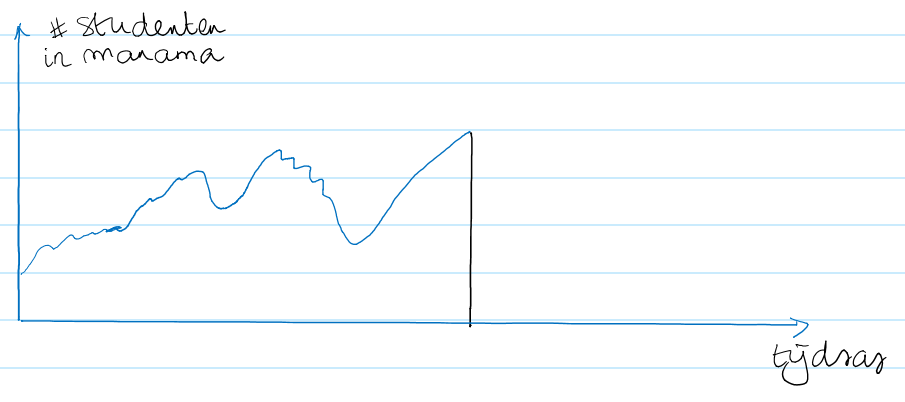
\includegraphics[width=90mm]{Les09_06.png}
\caption{Les 9 Slide 12} 
\label{les09_06}
\end{figure}

Met de zwarte informatie (niet de vervollediging van de grafiek) weet je meer. Het is hier zichtbaar hoe goed de markt is om een manama te doen. Uiteindelijk worden ze niet meer gesubsidi\"eerd, dus wordt deze uiteindelijk afgeschaft. Dit kon je niet weten/voorspellen vanuit de blauwe curve alleen, zonder info.

\paragraph{Slide 13:} Als je een curve analyseert, moet je dus rekening houden met alle gegevens die beschikbaar zijn. Maak ook altijd figuren, want het oog kan dingen afleiden die anders niet duidelijk zouden worden.

\paragraph{Slide 14:} Wanneer we zaken analyseren, gaan we een onderscheid maken tussen verschillende soorten processen. In deze slide kan je zien dat er ongeveer een constante is, waarbij we de ruis weglaten. 

\paragraph{Slide 15:} Het kan ook zijn dat we een bepaalde trendlijn hebben, of dat er een seizoensinvloed is. Het is ook mogelijk dat uw seizoensinvloed in stijgende lijn gaat. 

\paragraph{Slide 17:} Je mag ``subjectief" hier niet negatief bekijken. Je kan gaan kijken op basis van verkoopsagenten. Je kan gebruik maken van enqu\^etes die je rondstuurt. 

\paragraph{Slide 18:} Een enqu\^ete is een krachtig middel, maar het moet op de juiste manier gebruikt worden. Veel zaken lopen fout omdat er te weinig aandacht besteed wordt tijdens het opzetten. Je moet een vragenreeks opstellen zodat bepaalde punten naar voren komen en de vragen die je hebt beantwoord worden. Je moet zorgen dat de vragen eenduidig opgesteld zijn. Reeds bij het opstarten moet je kijken wat voor antwoorden je gaat krijgen en hoe je die gaat verwerken. Dan pas ga je die uitvoeren. Normaal gezien zal een 10-50\% van de aangesproken mensen reageren.\\
Als je een enqu\^ete rondstuurt, moet je zien dat die in orde is, je kan moeilijk vragen om ze nog eens in te vullen omdat er iets was misgelopen. De resultaten moet je gaan analyseren en interpreteren. Het is ook fijn voor de mensen die de enqu\^ete hebben ingevuld om te weten wat de resultaten zijn.

\paragraph{Slide 20:} Expertopinie: marketingmensen bij elkaar brengen, die weten wat er met een bepaalde markt zal gebeuren. Die kunnen dan samenzitten en discussi\"eren. Zij kunnen tot conclusies komen. Er zullen altijd een aantal mensen meer naar voor komen qua input, terwijl de anderen misschien ook interessante informatie hebben.\\
Er is ook een meer formele techniek, namelijk de Delphi-methode: de experten worden niet bij elkaar geplaatst maar ze zullen vragenlijsten binnenkrijgen die ze elk apart moeten beantwoorden. Zo krijg je geen interferentie. Dan ga je voorspellingen geven. Alle antwoorden die worden binnengebracht, worden samengevat en de mensen die het hebben ingevuld krijgen hun antwoorden en het gemiddelde, zodat ze hun antwoorden kunnen motiveren of aanpassen. Dit wordt herhaald tot men tot een convergentiepunt komt.

\paragraph{Slide 21:} Voordeel: verschillende achtergronden en weinig interferentie.\\
Nadeel: neemt heel veel tijd in beslag en het kan zijn dat je geen overeenkomst bereikt.

\paragraph{Slide 22 $\&$ 23:} Voorbeeld.

\paragraph{Slide 24:} Normaal, wanneer we kijken naar het resultaat hiervan, zullen we zien dat expertopinie meestal voldoende is. De Delphi-methode is tijdsverslindend en duur (je moet al die experts betalen). Bij ``gewone" correspondenten kan het goedkoper/gratis zijn, maar het kan langer duren vooraleer je antwoord hebt. 

\paragraph{Slide 25:} Als we kwantitatieve data hebben, zullen we ofwel van causale modellen gebruik maken, ofwel van tijdsreeksen. Bovenste zijn causale modellen, onderste zijn tijdsreeksen.

\chapter{Les 10: Oefenzitting 2}
\section{SlideS: Oefenzitting 2(1)}
Zie volgende pagina voor handgeschreven nota's.

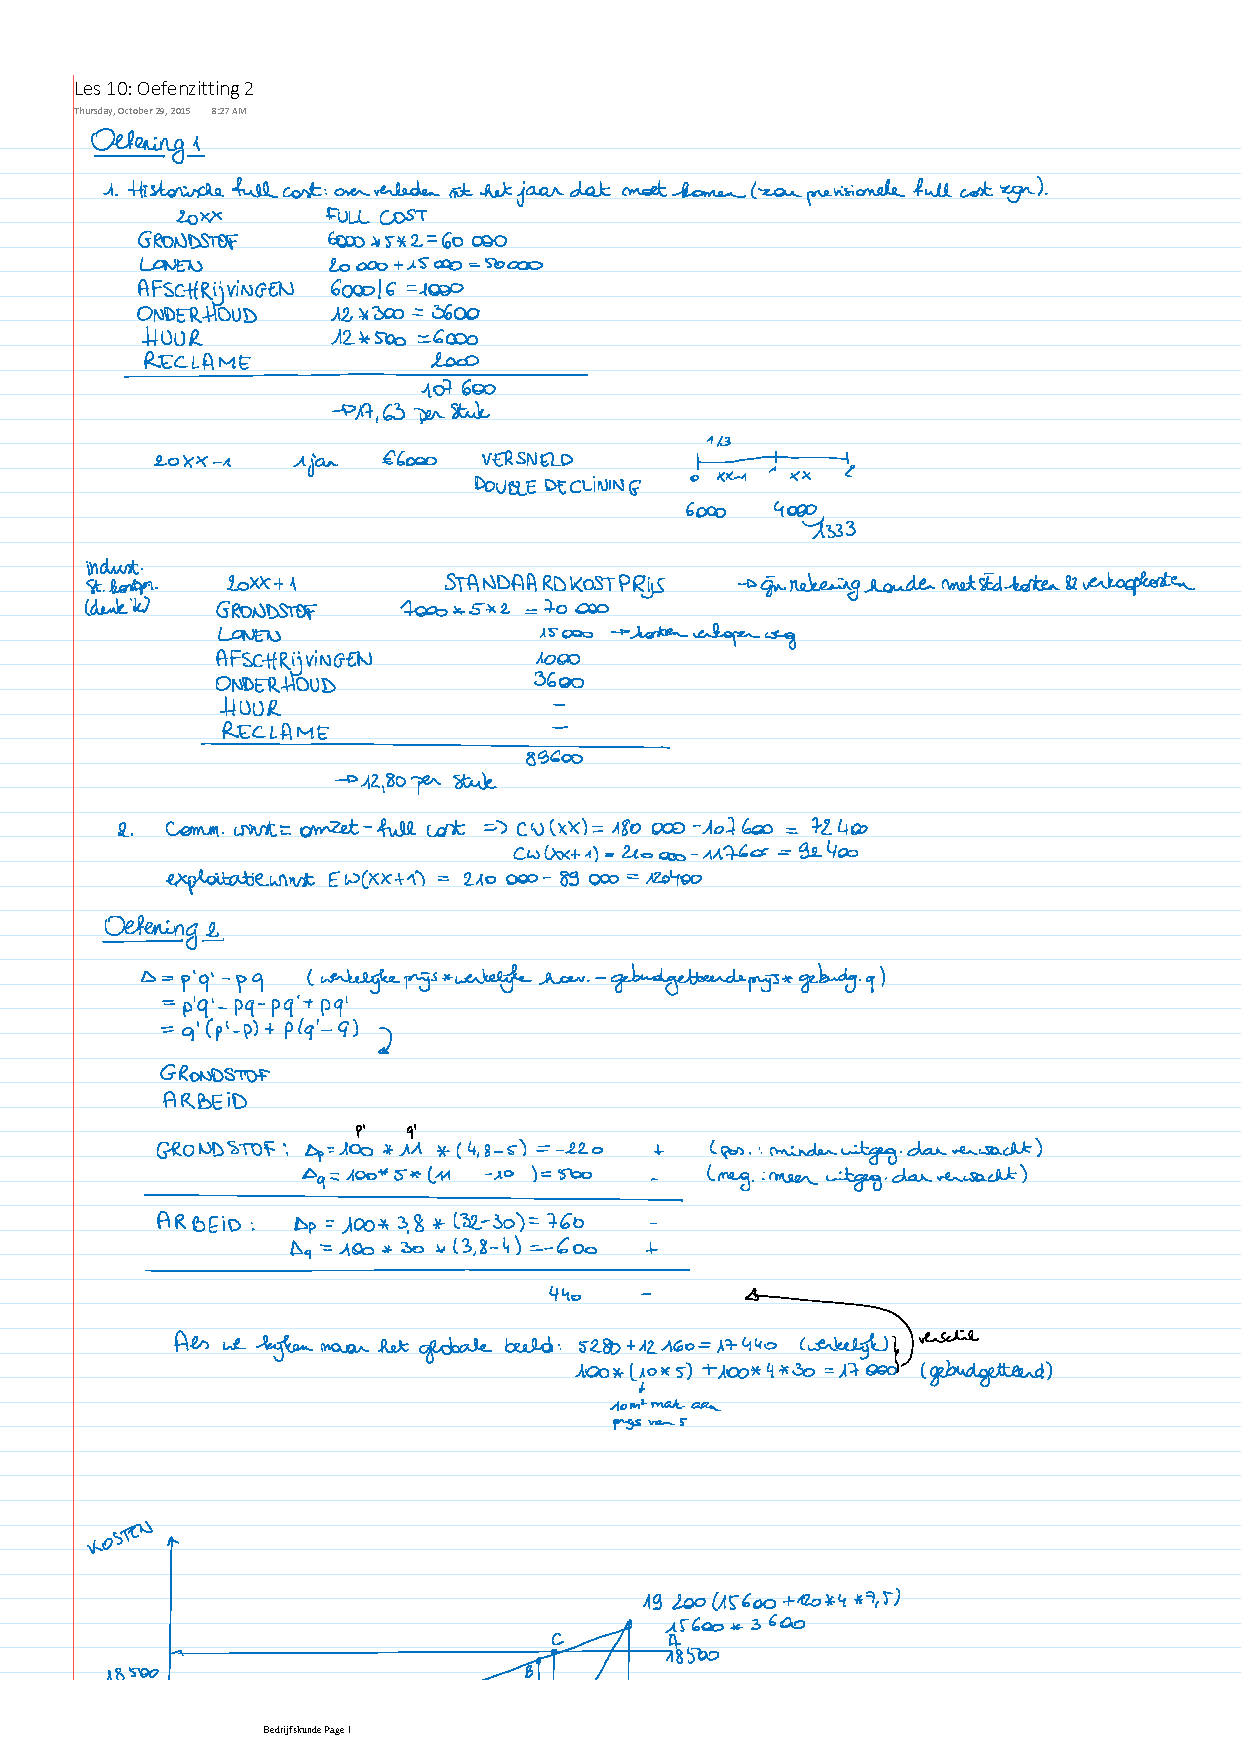
\includepdf[pages={1,2,3}]{Les10Oefenzitting2.pdf} 

\chapter{Les 11}

\section{Slides: 10\_Bedrijfskunde\_Voorspellingstechnieken}

\paragraph{Slide 25:} We gaan eerst kijken naar causale modellen: er gebeurt nu iets dat impact zal hebben op iets wat een paar maanden later gebeurt. We willen een verband leggen tussen wat nu gebeurt en wat later gebeurt.
Als er geen causaal verband is, maken we gebruik van tijdsreeksen gebaseerd op historische gegevens.\\
Belangrijk is om altijd een tekening te hebben als je historische gegevens hebt, zo kan je beter zien of er een trend is. De methode die je gebruikt zal afhankelijk zijn van het patroon dat je vindt. Als je een methode gebruikt die een trend niet kan weergeven, ga je een probleem hebben. Het is beter een methode te gebruiken die meer doet dan je verwacht. 

\paragraph{Slide 26:} D is de vraag in een bepaalde peroide, F is de voorspelling gemaakt op basis van de periodes op voorhand. Werken we met tijdsreeksen, baseren we ons op voorgaande vragen, rekening houdend met een bepaald gewicht. Naarmate de vraag verder in het verleden zit, zal het gewicht lichter zijn.

\paragraph{Slide 27:} We hebben een loodgieter die moet voorspellen hoeveel spanklemmen hij nodig gaat hebben. De eerste parameter is de onafhankelijke, de tweede is afhankelijk.

\paragraph{Slide 28:} De eerste methode die je kan gebruiken is lineaire regressie: de vraag die we hebben naar spanklemmen is een functie van het aantal bouwtoelatingen dat gegeven werd (h) vermenigvuldigd met een parameter b. We willen het volgende weergeven: zie Figuur \ref{les11_01}.\\

\begin{figure}[h!]
\centering
\includegraphics[width=90mm]{Les11_01.png}
\caption{Les 11 Slide 28} 
\label{les11_01}
\end{figure}

Let op dat je de juiste verbanden legt! Als kinderen meer tv kijken en ouders kopen meer paraplu's, is het een niet per s\'e het gevolg van het ander. Het kunnen alletwee gevolgen zijn van het feit dat het regent.

\paragraph{Slide 30:} Stellen we de gegevens van \textbf{Slide 29} grafisch voor, zien we inderdaad een lineair verband.\\
De bedoeling is nu om het snijpunt te vinden en dan de helling van de curve te vinden.\\
Hoe kunnen we dit doen? We kunnen dit op het zicht doen. Als we er een lijn doortrekken, kunnen we zien dat we starten op ongeveer 25. we hebben een stijging tot ongeveer 300, dus ongeveer 1,85 (rico). Als je 100 bouwplannen krijgt, zal je 25+185=210 spanklemmen nodig hebben.

\paragraph{Slide 31:} We kunnen ook telkens de fout ten opzichte van de rechte berekenen.

\paragraph{Slide 32:} De formules om de fout te vinden. Het resultaat blijkt 1,83 te zijn, hoewel de schatting 1,85 was. Dit toont dat de grafische methode vaak al genoeg is. Op het examen moet je de formules dus ook niet per s\'e gebruiken, de grafische methode is soms voldoende.\\
Ex-examenvraag: je hebt als vraag 98, 100, 102, 104, 106, 108, wat is het volgende getal in de rij? Ga niet die formules gebruiken, je ziet dat het met 2 stijgt, dus het volgende getal is 110.

\paragraph{Slide 33:} Er zijn ook andere regressiemethoden.

\paragraph{Slide 34:} Causale modellen zijn interessant wanneer er een verband is waarbij je 1 onderdeel kent en het andere wilt voorspellen.\\
Let op dat de zaken die je gebruikt vaak enkel bruikbaar zijn binnen bepaalde marges. Als je voor een bepaalde grootte van het product maar 1 persoon nodig hebt aan de machine, kan het zijn dat als het product groter wordt, je 2 mensen nodig hebt, dus gaat uw curve niet meer kloppen.

\paragraph{Slide 35:} Dikwijls hebben we geen causaal model en moeten we ons baseren op basis van tijdsreeksen. We beginnen met stationaire tijdsreeksen: constante processen. We nemen aan dat de vraag constant is en epsilon gelijk is aan de ruis.

\paragraph{Slide 36:} We gaan kijken naar de vorige periodes, die vragen optellen en dan delen door het aantal. Je moet wel bepalen welke input je neemt en we gaan ook kijken naar de invloed van die N.

\paragraph{Slide 37:} We kijken naar de verkoop van tandpasta. 

\paragraph{Slide 38:} De vraag van tandpasta weergegeven. Als we de voorspelling zouden willen maken voor periode 51 op basis van 3 periodes: zie Figuur \ref{les11_02}.

\begin{figure}[h!]
\centering
\includegraphics[width=90mm]{Les11_02.png}
\caption{Les 11 Slide 38} 
\label{les11_02}
\end{figure}

\paragraph{Slide 40:} De donkere curve is het vraagpatroon. We hebben nog een gele en roze curve. Het driewekelijkse gemiddelde zal starten na 3 weken (dus roze), het zeswekelijkse gemiddelde zal na 6 weken starten. Het gele is daarenboven meer uitgevlakt en genereert een stabieler patroon dan het roze. In de gele curve neem je meer getallen mee, waardoor het meer uitgevlakt zal zijn. Als je 3 keer 10 neemt, krijg je een gemiddelde van 10. als je 10, 10, 20 neemt, krijg je 13,3. Als we zouden kijken naar 6 perioden, zal een afwijking (van die 10) veel minder uitgesproken zijn. 

\paragraph{Slide 41:} Kijken we naar dezelfde vraag waarbij de concurrentie in rekening genomen moet worden: we zien een stijging in de vraag. Kijken we hier naar de 2 patronen: het driewekelijks gemiddelde zal sneller reageren dan het zeswekelijks gemiddelde omdat in het driewekelijks gemiddelde getallen sneller `verdwijnen' (je neemt ze sneller niet meer in rekening), het zeswekelijks gemiddelde zal langer blijven werken met oudere getallen. Als er wijzigingen zijn, zal het zeswekelijks gemiddelde dus achterlopen op het driewekelijkse gemiddelde.

\paragraph{Slide 42:} Wanneer we trends hebben, zal het voortschuivend gemiddelde continu achterlopen bij een stijging en voorlopen bij een daling.

\paragraph{Slide 43:} Voordeel: stabiel. Nadelen: je moet kijken of er een trend is of niet en bepaalde zaken worden niet in rekening gehouden, zoals complexe relaties, die hierin niet kunnen worden meegenomen.

\paragraph{Slide 44:} Tweede techniek om stationaire reeksen te voorspellen: exponenti\"ele afvlakking. We gaan elke keer een gewogen gemiddelde berekenen: we maken een bepaalde voorspelling, krijgen een bepaalde vraag die normaal zal afwijken en we gaan dat lineair interpoleren en op basis daarvan een nieuwe vraag afleiden. Het komt er dus op neer dat we een gewogen gemiddelde nemen tussen de gekende vraag en de voorspelling. We moeten weer een gewicht geven aan de gekende vraag en het voorspelde getal. De nieuwe voorspelling zal gelijk zijn aan $\alpha$. 

\paragraph{Slide 45:} $\alpha$ zal men meestal liggen rond 0,1, 0,2. Als je $\alpha$ groter maakt, zal je veel meer variabel rondspringen. Als $\alpha$ kleiner is, zal je een veel stabieler patroon hebben. Als je de eerste formule uitschrijft als $F_{t-1}$ en $D_{t-1}$, zie je dat we rekening houden met alle voorbije data. De factor waarmee we rekening houden met het verleden wordt wel kleiner met de tijd. 

\paragraph{Slide 46:} Je ziet dat oude data steeds minder gewicht krijgt.
Voorbeeld: zie Figuur \ref{les11_03}.

\begin{figure}[h!]
\centering
\includegraphics[width=90mm]{Les11_03.png}
\caption{Les 11 Slide 46} 
\label{les11_03}
\end{figure}

\paragraph{Slide 47:} Als er een trend is, lopen beide methoden achter. ES houdt rekening met alle voorbije data, met telkens minder gewicht. Het grote voordeel van het voortschrijdend gemiddelde is dat als er ergens een piek is (meetfout bv.), dan zal die na enkele periodes niet meer in rekening genomen worden. 

\paragraph{Slide 48:} We hebben voor de voorbije 24 maanden de verkopen staan. Als we kijken naar de cijfers die er staan, merken we dat de waarden stijgen en er zal wellicht ergens een trend inzitten. We kunnen dit oplossen met regressieanalyse, maar expoleren is gevaarlijk.

\paragraph{Slide 49:} Komen we een curve zoals deze tegen, gaan we dubbele exponenti\"ele afvlakking gebruiken. Het is de bedoeling om de trend te vinden (lineair) die er is.

\paragraph{Slide 51:} Het komt erop neer dat wanneer we kijken naar een voorspelling, we ergens een startpunt hebben en ergens een bepaalde trend (zie tekening). Op basis van het startpunt en de trend zullen we uiteindelijk onze voorspelling bekomen. Zie Figuur \ref{les11_04}.\\

\begin{figure}[h!]
\centering
\includegraphics[width=30mm]{Les11_04.png}
\caption{Les 11 Slide 51 (1)} 
\label{les11_04}
\end{figure}

In de eerste vergelijking, $S_{t-1} + G_{t-1}$ komt overeen met $F_{t}$. Ons nieuw startpunt zal overeenkomen met de voorspelling aan de ene kant en de vraag aan de andere kant.\\
De volgende helling wordt bepaald door de trend van de vorige periode, het verschil tussen de twee startpunten (stippellijn op Figuur \ref{les11_05}). We zullen een weging maken tussen de oorspronkelijke trend en de trend veroorzaakt door de 2 startpunten. Dan vertrekken we daaruit en krijgen we $G_{t}$. Zie Figuur \ref{les11_05}.

\begin{figure}[h!]
\centering
\includegraphics[width=90mm]{Les11_05.png}
\caption{Les 11 Slide 51 (2)} 
\label{les11_05}
\end{figure}

\paragraph{Slide 52:} We willen een voorspelling maken. We moeten ergens op een of andere manier een startpunt vinden ($S_{24}$) en een $G_{24}$ zodanig dat als we $S_{24}$ en $G_{24}$ optellen, we $F_{25}$ krijgen.\\
We kunnen dit op verschillende manieren doen: grafisch (lijn trekken en dan aflezen op de grafiek). We moeten hierbij dan een goede trend vinden en een start bepalen.\\
We hebben 2 jaren gegeven. De trend over 2 jaar heen is ongeveer dezelfde. Als we daarmee starten, kunnen we het volgende doen: zie Figuur \ref{les11_06}.\\

\begin{figure}[h!]
\centering
\includegraphics[width=90mm]{Les11_06.png}
\caption{Les 11 Slide 52 (1)} 
\label{les11_06}
\end{figure}

Kijken we naar deze cijfers: als je een overschatting maakt, gaat alles naar beneden getrokken worden, maak je een onderschatting, wordt alles naar boven getrokken. Zie Figuur \ref{les11_07}.\\

\begin{figure}[h!]
\centering
\includegraphics[width=90mm]{Les11_07.png}
\caption{Les 11 Slide 52 (2)} 
\label{les11_07}
\end{figure}

We kunnen dus op verschillende manieren starten. Wat we ook kunnen doen is Holt toepassen van in het begin. Je moet wel ergens een beginwaarde en begintrend vinden. Je kan dan een formule toepassen waarbij je de trend en het startpunt aanpast en zo een nieuw punt vindt. De voorspelling is dus de som van uw trend en uw startpunt.\\
Nu is het zo dat je andere waarden kan nemen als beginwaarde, dan zal je merken dat op het einde de afwijking relatief klein is. Als je in het begin ergens een fout hebt gemaakt, zal zich dat uitvlakken omdat oude informatie steeds minder hard zal doorwegen. 

\paragraph{Slide 53:} We hebben ook seizoensinvloeden. Het is dan interessant om te kijken naar de periodes waarin ze terugkeren. Je kan seizoensinvloeden hebben die over een jaar zijn (bv. speelgoedfabrikanten), maar ook om de zoveel maanden. Je moet dit eerst proberen te herkennen vanuit uw data. Dan ga je een formule opstellen.

\paragraph{Slide 55:} We gebruiken altijd hetzelfde systeem: we hebben ergens een bepaald startpunt, een bepaalde trend en dan krijg je een punt op de trendlijn en moet je de seizoensfactor introduceren (factor $>$1 of $<$1). In dit geval hebben we een seizoensinvloed die gekoppeld is aan een trend. Zie Figuur \ref{les11_08}.

\begin{figure}[h!]
\centering
\includegraphics[width=90mm]{Les11_08.png}
\caption{Les 11 Slide 55} 
\label{les11_08}
\end{figure}

\paragraph{Slide 56:} Gelijkaardige formules. $S_{t}$ = startpunt, $G_{t}$ = de helling, $c_{t}$ = seizoensinvloed. We gaan de vraag delen door de seizoensfactor (D/c) zodat we het verschil hebben.\\
Als het vraagpatroon er als volgt zou uitzien, dan gaan we niet de zwarte periodes nemen. We gaan het eerste deel aan de kant laten liggen, die zijn niet representatief. Het kan zijn dat je pas na een tijd een normale vraag krijgt. Zie Figuur \ref{les11_09}. \\

\begin{figure}[h!]
\centering
\includegraphics[width=90mm]{Les11_09.png}
\caption{Les 11 Slide 56} 
\label{les11_09}
\end{figure}

Als je het eerste deel meeneemt, ga je te lang nodig hebben om je aan te passen en de fout weg te werken.

\paragraph{Slide 58:} Formules.

\paragraph{Slide 59:} Voorbeeld: We hebben de periodes t, de vraag d en de voorspelling F gekoppeld aan die vraag d. e = F-d. E is de cumulatieve fout. MAD is de absolute waarde van het gewogen gemiddelde. MSE is de gemiddelde foutmarge in het kwadraat. MAPE zijn de percentages.\\
Wat kunnen we zeggen over de e-kolom? We moeten zowel positieve als negatieve waarden hebben. Als we altijd een positieve of negatieve fout vinden, gaan we voorlopen. Het is niet zo dat we graag kleine negatieve en grote positieve waarden hebben. We willen dat als we de som gaan bekijken, we ongeveer 0 uitkomen. Als de waarden in E zowel positief als negatief zijn, is dat ook goed. Je wilt waarden vinden die positief en negatief zijn en liefst zo dicht mogelijk bij nul liggen. Bij MAD, MSE en MAPE hebben we graag waarden die stabiel worden na een bepaalde periode. Kijken we naar de gemiddelde fout en de gemiddelde kwadratische fout, deze mogen niet plots beginnen stijgen, want dan krijgen we plots grote afwijkingen. We willen dus dat die waarden relatief stabiel zijn. MAPE moet ook stabiel zijn, dat geeft ons weer wat onze gemiddelde afwijking is.\\
Als we tot de conclusie komen dat bepaalde zaken totaal fout lopen, moeten we de zaken analyseren.

\paragraph{Slide 60:} Bias: constant positief of negatief. 

\paragraph{Slide 61:} Om dit te kunnen opvolgen maakt men gebruik van quality management. We willen dat onze fout binnen een bepaalde marge zit (komt niet op examen, ter informatie). Er is een verband tussen de gemiddelde absolute afwijking en de $\sigma$ van de ruis. De $\sigma$ van de ruis is ongeveer de gemiddelde afwijking/0,8. Voor de $\alpha$-waarden kom je dan ook tot een bepaald verband.\\
Uiteindelijk is het zo dat we ergens een fout zullen maken en dat we proberen die fout te krijgen tussen 2 waarden. Zolang onze fout tussen die twee waarden zit, zullen we aannemen dat onze voorspellingstechniek goed werkt. Zitten we buiten die waarden, dan moeten we gaan reageren en nakijken wat er verkeerd loopt met onze methode of wat er is aangepast aan het vraagpatroon. 

\paragraph{Slide 62:} Om dit te kunnen doen, maken we voorspellingen op de fouten. Zolang $\rho$ kleiner of gelijk is aan 4, zitten we goed. 

\paragraph{Slide 64:} We gaan de voorspellingen genereren en doorrekenen. We zien dan dat $\rho$ altijd kleiner is dan 4. In dit geval zitten we betrouwbaar en hebben we geen enkel probleem. Onze voorspellingsmethode werkt dus goed.

\paragraph{Slide 66:} Bij exponenti\"ele afvlakking zijn er problemen als er een plotse sprong is. Exponenti\"ele afvlakking kan het dus niet volgen.\\
We doen dezelfde berekeningen (\textbf{Slide 67}) en zien dat onze delta (voorspelling van de fout) dit toont, alsook rho: rho komt boven de 4. Als je dat merkt, wil dat zeggen dat je moet reageren, je moet nakijken wat er fout loopt.\\
Wil het zeggen dat als je boven 4 zit, er een foute methode wordt gebruikt? Niet noodzakelijk. Het kan zijn dat er iets gebeurd is waardoor we plots een grote rho krijgen. Het kan zijn dat er een sprong is geweest, maar achteraf opnieuw een stabiel patroon. We moeten gewoon kijken wat er gebeurd is, en eventueel geen rekening houden met die sprongen. 

\paragraph{Slide 68:} Je moet niet plots nieuwe methoden gebruiken, gewoon eerst kijken wat er gebeurd is en dan handelen. Je kan dan bepaalde cijfers schrappen en initaliseren met nieuwe waarden.\\
Kijken we op het einde naar de waarden (\textbf{Slide 67}), zien we rho weer dalen naar het einde toe.

\paragraph{Slide 70:} Het is van groot belang om na te gaan welk model gebruik moet worden. Je moet dit ook opvolgen, niet gewoon starten en dan zo verder werken, je moet altijd controleren.\\
We hebben zeer eenvoudige modellen gezien, er zijn er natuurlijk ook complexere. 

\paragraph{Slide 72:} Onze voorspelling zal juist zo zijn dat we die nodig hebben voor ons voorraadbeheer en ons productieplan. Kijken we naar de voorraad, kijken we naar de eindvoorraad. Als die eindvoorraad is vastgelegd, gaan we daaraan de productie koppelen. Bij de inventory gaan we andere assumpties maken dan bij de productie.

\chapter{Les 12}
\section{Slides: 11\_Bedrijfskunde\_Productie- en voorraadcontrolesystemen(1)}

\paragraph{Slide 2:} We gaan een voorraadpolitiek vastleggen. Op basis daarvan kijken we naar het productieplan zelf. De eerste 4 systemen worden allemaal gebruikt om productie aan te sturen. 

\paragraph{Slide 4:} Voorraadbeheer is van belang omdat de verkoop (en voorraad) gekoppeld is aan de financi\"ele cyclus van het bedrijf. We willen dat de voorraadrotatie klein is zodat de financi\"ele cyclus ook klein is. Het is de bedoeling dat de cirkel zo snel mogelijk rond is en het geld zo snel mogelijk opnieuw binnenkomt.

\paragraph{Slide 5:} We gaan kijken naar voorraden omdat zelfs als de vraag volledig deterministisch en gekend zou zijn, we toch gebruik gaan maken van voorraden. De redenen zijn gegeven in het lijstje:
\begin{itemize}
\item Schaalvoordelen: naarmate we meer stuks maken, kunnen we de vaste kosten verdelen over al die stuks, waardoor de kost per stuk lager is: zie Figuur \ref{les12_01}.

\begin{figure}[h!]
\centering
\includegraphics[width=90mm]{Les12_01.png}
\caption{Les 12 Slide 5 (1)} 
\label{les12_01}
\end{figure}	
	
\item Onzekerheid in levertermijn: er zit een bepaalde spreiding op wanneer de leverancier levert. Je moet zorgen dat als de leverancier aan de late kant is, je toch nog kan produceren.
\item Speculatie: als je weet dat accijnzen bv. gaan stijgen, ga je voorraden aanleggen.
\item Transport
\item Uitvlakken productie: zie Figuur \ref{les12_02}.

\begin{figure}[h!]
\centering
\includegraphics[width=90mm]{Les12_02.png}
\caption{Les 12 Slide 5 (2)} 
\label{les12_02}
\end{figure}

\item Logistiek
\item Controlekosten: je moet betalen per controle, dus als je meer kan laten controleren in een keer, zal het goedkoper zijn.
\end{itemize}

\paragraph{Slide 6:} We moeten altijd controleren hoe we verkopen: soms meer, soms minder. We moeten continu controleren wat er gebeurt met de voorraad. 

\paragraph{Slide 7:} Er bestaan verschillende systemen. Het eerste gaat periodiek kijken wat er gebeurt met de voorraad. Ongeacht wat er gebeurt, we gaan pas kijken op $t_{1}$ en daarna op $t_{2}$. We merken dat we een target niveau hebben (max. niveau van voorraad dat we willen), maar ook een reorder point: zodra we hieronder komen, gaan we bijbestellen. De restvoorraad zal onvoldoende zijn om de cyclus te overbruggen. Je bemerkt dat we controleren op $t_{1}$ en $t_{2}$, bij $t_{2}$ zien we dat we moeten bijbestellen. Het kan ook zijn dat de voorraad veel drastischer gaat dalen, waarbij je negatieve voorraad kan hebben, waarbij je niet kan voldoen aan de vraag. \\
Een ander systeem is het continu herzien: continu kijken in ons magazijn hoe de voorraad is. We zien dat onze voorraad daalt en dat we ons reorder point naderen, dus we gaan opnieuw bijbestellen. Als de voorraad nu heel snel daalt, gaan we snel kunnen bijbestellen. \\
Het systeem van continu herzien zal veel duurder zijn dan periodiek herzien. Men gebruikt bij continu herzien vaak RFID of barcodes. Men zal continu herzien gebruiken voor kritieke stukken, wanneer tekorten daarbij grote implicaties heeft voor de klanten. Voor standaardstukken ga je periodiek herzien gebruiken, waarbij het wel eens (een beetje) mag foutlopen.

\paragraph{Slide 8:} Aan de ene kant is het nuttig om zoiets te hebben omdat we zo flexibel kunnen zijn, maar anderzijds gaan we ook een hele reeks kosten hebben. Die kosten hebben te maken met
\begin{itemize}
\item opslag: daar zit geld in dat niet gebruikt kan worden. Dit wordt dikwijls uitgedrukt in procenten: hoeveel procent van de voorraad zal voor een bepaalde bestelling gebruik worden?
\begin{itemize}
\item Verouderingskosten: als producten ergens lang liggen, gaan klanten dat misschien niet meer willen. Het kan zijn dat er producten zijn die niet meer roteren in het bedrijf. Ze zijn niks meer waard voor de klant, maar het bedrijf houdt ze omdat ze anders de balans moeten aanpassen.
\item Diefstal: als er taarten worden gemaakt in de winkel, kan het zijn dat het personeel versieringen ofzo zelf opeet.
\end{itemize}
\item voorraadbreukkosten: het kan zijn dat men zegt dat er per dag te laat een bepaalde boete betaald wordt, of dat je die klant verliest. Op die manier kan je eventueel ook andere klanten verliezen omdat je niet betrouwbaar bent. Je kan werken met een service graad: men gaat proberen een voorraadniveau te halen zodat je in 95\% van de gevallen kan leveren aan je klant.
\item orderkosten: gegevens ingeven, kijken wat er gebeurt aan de los- en laadkade.
\item opvolging: software/hardware om bv. te kijken welke boeken in een bibliotheek binnenkomen/buitengaan kost ook geld.
\end{itemize}

\paragraph{Slide 9:} Als we kijken naar kosten moeten we 2 zaken afwegen: voorraadkosten en naarmate de lotgrootte stijgt, zullen we grotere voorraden krijgen. Kleinere batches zorgen voor kleinere voorraadkosten, maar dit kan zorgen voor grotere omstelkosten (== bestelkosten). Het is de bedoeling om die 2 tegenover elkaar af te wegen. Als je de totale kost neemt, ga je het minimum zoeken en dat is het punt waarbij je totaal genomen de kleinste voorraadkost en bestelkost hebt. 

\paragraph{Slide 10:} We hebben verschillende soorten modellen. Wij gaan enkel kijken naar de statische modellen. Voor de dynamische heb je modelleringsmodellen nodig.\\
We gaan voorbeelden bekijken waarbij we kijken naar uniforme constante vraag over de tijdshorizon. Hierbij gaan we kijken naar het eindproduct en niet naar de onderliggende delen. %TODO Als jenaar de onderliggende delen kijkt (? 17.00).

\paragraph{Slide 11:} We beginnen met het basismodel. We nemen aan dat de vraag gekend, deterministisch en constant is. De lotgrootte q gaan we proberen te bepalen. Deze is constant en wordt bijgesteld wanneer nodig. De voorraad wordt bijgevuld wanneer het voorraadniveau 0 is. We nemen aan dat de doorlooptijd om de voorraad heraan te leggen 0 is (dus nieuwe voorraad wordt besteld en is direct in huis).

\paragraph{Slide 12:} Zaagtandpatroon: elke keer als de voorraad 0 is, bestellen we bij. Dan halen we producten uit het magazijn. De vraag is constant dus het verloopt lineair. We gaan een bepaalde cyclus hebben en na periode T bestellen we bij.

\paragraph{Slide 13:} We hebben voorraadkosten die gekoppeld zijn aan de batchkosten en de periodes T. Die gaan we moeten afwegen tegenover elkaar.\\ 
Kijken we naar onze gegevens, dan hebben we een bepaalde kost r, we kopen het product aan aan een kost c. We merken dat die totaal onafhankelijk is van onze batchgrootte (we krijgen geen korting bij grotere hoeveelheden). Dat is onze aankoopkost. We zullen een orderkost hebben en een voorraadkost. De voorraadkost is gegeven en de orderkost ook (op de vorige slide). De vraag is nu wat de voorraadkost is. Zie Figuur \ref{les12_03}.\\

\begin{figure}[h!]
\centering
\includegraphics[width=90mm]{Les12_03.png}
\caption{Les 12 Slide 13 (1)} 
\label{les12_03}
\end{figure}

We willen de juiste waarden vinden voor A, dus: zie Figuur \ref{les12_04}.\\

\begin{figure}[h!]
\centering
\includegraphics[width=90mm]{Les12_04.png}
\caption{Les 12 Slide 13 (2)} 
\label{les12_04}
\end{figure}

Naarmate de orderkost groter wordt, willen we minder bestellingen plaatsen, dus grotere batches (vandaar $c_{p}$ in de teller). Als de voorraadkosten groter worden, gaan we minder voorraad willen hebben, dus daarom $c_{h}$ in de noemer.\\
Bekijken we een paar specifieke zaken verder: zie Figuur \ref{les12_05}.

\begin{figure}[h!]
\centering
\includegraphics[width=90mm]{Les12_05.png}
\caption{Les 12 Slide 13 (3)} 
\label{les12_05}
\end{figure}

\paragraph{Slide 14:} De vraag is gekend, dus je kijkt hoe lang het duurt voor je voorraad voor x dagen opgebruikt is. Je bestelt op voorhand zodat je geen voorraadtekort krijgt.

\paragraph{Slide 15:} Je moet ervoor zorgen dat alle gegevens er staan met de juiste dimensies. Spreken we over jaarvragen, moeten we ook kijken naar jaarlijkse opportuniteitskosten. We gaan het voorbeeld uitwerken:

\begin{figure}[h!]
\centering
\includegraphics[width=90mm]{Les12_06.png}
\caption{Les 12 Slide 15 (1)} 
\label{les12_06}
\end{figure}

\begin{figure}[h!]
\centering
\includegraphics[width=90mm]{Les12_07.png}
\caption{Les 12 Slide 15 (2)} 
\label{les12_07}
\end{figure}

\paragraph{Slide 16 e.v.:} Marvin kan beter meer bestellen.

\paragraph{Slide 18:} We kunnen ook zelf onderdelen gaan produceren, maar dan zijn die onderdelen niet meteen beschikbaar, het duurt een bepaalde tijd vooraleer ze geproduceerd zijn. De vraag is nu of onze productiebatch groter of kleiner gaat zijn. Nemen we in de piek H als de hoogte van de voorraad: zie Figuur \ref{les12_08}. \\

\begin{figure}[h!]
\centering
\includegraphics[width=90mm]{Les12_08.png}
\caption{Les 12 Slide 18 (1)} 
\label{les12_08}
\end{figure}

Als p oneindig is, zijn die twee aan elkaar gelijk (q en H).
We kunnen de formule dus omvormen tot: zie Figuur \ref{les12_09}.\\

\begin{figure}[h!]
\centering
\includegraphics[width=50mm]{Les12_09.png}
\caption{Les 12 Slide 18 (2)} 
\label{les12_09}
\end{figure}

p moet groter zijn dan r, anders kan de productie niet voldoen aan de vraag.

\paragraph{Slide 20:} We kijken eerst naar een systeem waarbij we korting krijgen voor alle eenheden die we aankopen, daarna naar modellen waarbij we korting krijgen vanaf een bepaalde hoeveelheid.\\
Kijken we naar een verduidelijkend voorbeeld: zie Figuur \ref{les12_10}.

\begin{figure}[h!]
\centering
\includegraphics[width=90mm]{Les12_10.png}
\caption{Les 12 Slide 20 (1)} 
\label{les12_10}
\end{figure}

De $r_{c}$ zal nu wel vari\"eren, zal een functie zijn van q. Hier zal het dus afhankelijk zijn van onze bestelgrootte.\\
Als we aannemen dat de drie kostenfuncties alledrie geldig zijn en we tekenen de volledige kostenfunctie uit, dan merken we dat we 3 curvers hebben, waarbij die met de hoogste aankoopkost bovenaan ligt en de laagste aankoopkost onderaan. Die curvers snijden elkaar niet in de tweede figuur. De curves zijn enkel geldig in de gemarkeerde gebieden: zie Figuur \ref{les12_11}.\\

\begin{figure}[h!]
\centering
\includegraphics[width=90mm]{Les12_11.png}
\caption{Les 12 Slide 20 (2)} 
\label{les12_11}
\end{figure}

Hoe kunnen we nu starten om de optimale oplossing te vinden? \\
De drie curves snijden mekaar niet en $c_{3}$ is de laagste en de andere twee liggen erboven. Als dit voldoet aan de voorwaarden, moet je de andere curven niet meer bekijken want het optimum ligt in het minimum van $c_{3}$. We zullen dus onderaan starten met de derde curve en kijken of dat optimale punt voldoet aan de eisen. Als het aan de rand ligt zoals op de afbeelding, zijn we niet zeker of het laagste punt daar lager ligt dan bij de tweede laagste. Is dit buiten het bruikbaar gebied, ga je weer naaar boven werken.\\
We bemerken ook dat als we de 3 curves met elkaar vergelijken, dan verschuift het minimum naar links. \\
Als we de curven tekenen en de aankoopkosten wijzigen, dan wijzigen ook de curven. Als de aankoopkost daalt, daalt de voorraadkost, zal de optimale hoeveelheid stijgen: zie Figuur \ref{les12_12}.\\

\begin{figure}[h!]
\centering
\includegraphics[width=90mm]{Les12_12.png}
\caption{Les 12 Slide 20 (3)} 
\label{les12_12}
\end{figure}

Voorbeeld: zie Figuur \ref{les12_13}.\\

\begin{figure}[h!]
\centering
\includegraphics[width=90mm]{Les12_13.png}
\caption{Les 12 Slide 20 (4)} 
\label{les12_13}
\end{figure}

We hebben hier dus het minimum van de onderste curve genomen.\\
We zijn niet zeker dat we het optimale punt hebben, dus we berekenen $q_{2}^{*}$: zie Figuur \ref{les12_14}. \\

\begin{figure}[h!]
\centering
\includegraphics[width=90mm]{Les12_14.png}
\caption{Les 12 Slide 20 (5)} 
\label{les12_14}
\end{figure}

Bij $q_{*}^{3}$ kopen we voor meer dan een jaar aan voorraad, je moet dan zeker zijn dat er geen plotse daling in verkopen zal zijn. Soms is het dus beter om het duurdere ($q_{2}^{*}$ in dit geval) te nemen, omdat je minder voorraad zal overhebben. Een verschil van 5 is vrij klein, dus het is zeker werkbaar. Je moet altijd kijken naar alle factoren. In dit geval is het dus beter om iets meer te betalen maar minder lang met voorraden te zitten.

\paragraph{Slide 21:} Bij incrementele korting gaan de curves mekaar snijden. Men heeft kunnen bewijzen dat de snijpunten nooit optimaal kunnen zijn. We gaan intu\"itief bekijken hoe de formule in elkaar zit.
We moeten alle kostencurves doorrekenen en enkel de kostencurves waarbij we een optimum vinden binnen de marges, daarmee gaan we verder werken. We gaan hier ook werken met de EOQ-formule.\\
Uw voorraadwaarde gaat hier niet meer lineair zijn zoals bij alle eenheden die korting krijgen.\\
We komen tot volgende formule: zie Figuur \ref{les12_15} $\&$ \ref{les12_16}.

\begin{figure}[h!]
\centering
\includegraphics[width=90mm]{Les12_15.png}
\caption{Les 12 Slide 21 (1)} 
\label{les12_15}
\end{figure}

\begin{figure}[h!]
\centering
\includegraphics[width=90mm]{Les12_16.png}
\caption{Les 12 Slide 21 (2)} 
\label{les12_16}
\end{figure}

\paragraph{Slide 22:} Dikwijls zal het zo zijn dat er beperkingen zijn (we hebben niet maar 1 product bv.) en zal er interactie zijn tussen verschillende systemen. We gaan hierbij gebruik maken van lagrange-relaxatie. Zie Figuur \ref{les12_17}.

\begin{figure}[h!]
\centering
\includegraphics[width=90mm]{Les12_17.png}
\caption{Les 12 Slide 22} 
\label{les12_17}
\end{figure}

Je kan lambda bepalen, maar de noemers zijn aan elkaar gelijk. Wanneer je zit met een budgetbeperking zal die evenredig zijn over de verschillende producten (denk ik).\\
We vinden dat $q_{1}$ = 36 en $q_{2}$ = 40. Ze zijn op een gelijkaardige manier gedaald. \\
Op die manier kan men relaties inbrengen waarbij producten aan elkaar gekoppeld zijn. Men kan ook meerdere beperkingen inbouwen.

\chapter{Les 13}
\section{Slides: Slides: 11\_Bedrijfskunde\_Productie- en voorraadcontrolesystemen(1)}

\paragraph{Slide 25:} We hebben de basis gezien van economische ordergrootte. We hebben gekeken naar kortingen en bijkomende beperkingen zodanig dat items niet onafhankelijk van elkaar beschouwd kunnen worden. Als men bezig is met voorspellen of voorraadopvolging, gaat men niet alle items op dezelfde manier bekijken. Men zal het onderscheid maken tussen belangrijke en minder belangrijke stukken in het magazijn. Bij sommige stukken moet alles opgevolgd worden, bij andere kan men relaxter zijn.\\
Dit alles is gebaseerd op Pareto. Als je kijkt naar voorraden gaan we zien dat een kleine hoeveelheid voorraden zal zorgen voor zeer grote rotatie en voor geldomzet voor een bedrijf. Vandaar wordt een ABC analyse gemaakt (geen activity based costing), maar een onderverdeling in belangrijkheid van de goederen.

\paragraph{Slide 26:} Voorbeeld: 29037 producten in het magazijn die gerangschikt zijn op geldwaarde. Tot aan product 10 gaan we met 1 naar boven, daarna met 15 naar boven en telkens met een grotere groep naar boven. We zien het aantal actieve producten in \% uitgedrukt. Het eerste product stelt eigenlijk niets voor qua percentage actieve items, maar het geeft wel de grootste omzet per jaar. De cumulatieve som toont dat 10\% van de producten zal verantwoordelijk zijn voor bijna 8\% van gebruik in het magazijn. \\
Het is soms interessant om items die lang in het magazijn blijven liggen te verkopen aan restwaarde en te vervangen door items die minder lang in het magazijn liggen. Bedrijven doen dit vaak niet omdat ze dat ingeschreven hebben aan een bepaalde kostprijs en ze moeten dat dan verkopen aan bijna niks.\\
Voor de eerste groep van items ga je zorgen dat je een hoge service graad hebt. De items achteraan, daar kun je iets rustiger mee zijn, maar wel nog mee oppassen: het is niet omdat een stuk een kleine rotatie heeft, dat het niet belangrijk is.

\paragraph{Slide 27:} Ongeveer 8\% van de producten zorgt voor ongeveer 80\% van de rotatie. We moeten ook kijken naar de stukkken meest rechts. Het kan zijn dat dat wisselstukken zijn voor bepaalde belangrijke machines. Als de machine faalt betekent dat dat daar zware kosten voor zijn, dus die stukkken moeten wel op voorraad zijn.\\
A zeker grondig bekijken, bij C moet je nagaan of er iets kritiek is.\\
Die curves kunnen verschillende soorten vormen aannemen. Als ze zeer snel stijgt, zal je veel stukken hebben met hoge waarde. Bij hoogtechnologische producten zal men dit type curve hebben. Bij Carrefour bv. verkoopt men alles (computers, kleren, eten), bij hen zal de curve niet zo uitgesproken zijn, eerder vlakker (lineairder): zie Figuur \ref{les13_01}.

\begin{figure}[h!]
\centering
\includegraphics[width=90mm]{Les13_01.png}
\caption{Les 13 Slide 27} 
\label{les13_01}
\end{figure}

\paragraph{Slide 29:} We hebben een bepaald stuk, zeg A, dat samengesteld is uit B en C, die producten zijn ook onderverdeeld in andere onderdelen. Zie Figuur \ref{les13_02}.\\

\begin{figure}[h!]
\centering
\includegraphics[width=90mm]{Les13_02.png}
\caption{Les 13 Slide 29} 
\label{les13_02}
\end{figure}

We starten met de onafhankelijke vraag van product A en spreiden dit verder uit voor de onderliggende delen om ons product A samen te stellen. Voor A maken we de forecast. Eens we daarvoor onze productie hebben vastgelegd, gaan we op basis van die productie kijken naar de onderliggende niveau's.

\paragraph{Slide 31:} Eens we de planning en behoeftes hebben opgesteld voor het bovenste niveau, gaan we kijken naar onderliggende niveau's, naar MRP. We moeten rekening houden met voorraad, kijken naar welke machines nodig zijn. Eventueel moet de planning herzien worden en het meesterplan herzien worden. Als we dan bezig zijn met MRP krijgen we een output. Aan de ene kant zullen we orders vrijgeven op onze eigen werkvloer (beginnen met stukken te assembleren en verwerken) en aan de andere kant zullen we misschien zaken moeten aankopen zoals grondstoffen of halffabrikaten. Een keer als alles gepland is en we bezig zijn met uitvoeren, moeten we ook gaan controleren. Het is niet omdat je een plan hebt, dat alles uitgevoerd wordt volgens plan (machines kunnen kapot gaan,…). Orders worden pas vrijgegeven als alles vrijgegeven kan worden.\\
Als bepaalde stukken niet gemaakt kunnen zijn, moet je de planning en voorraden aanpassen en opnieuw starten. Vandaar de lus.

\paragraph{Slide 32:} Als we bezig zijn met dergelijke zaken, gaan we werken op een geaggregeerd niveau. Dikwijls werkt men met light, medium and high trucks.\\
Als men 100 light trucks moet maken, zal men zoveel procent van dat nodig hebben en zoveel van dat.\\
Je houdt rekening met de voorraad reeds aanwezig en je houdt rekening met capaciteitsbeperkingen en doorlooptijden. Als we een bepaald stuk in eind januari willen hebben, kan het zijn dat je lang op voorhand moet starten wegens een lange productieduur. 

\paragraph{Slide 33:} Je moet ook kijken welk type bedrijf je hebt en welk type markt. We moeten hier een afweging maken tussen doorloopkosten en flexibiliteit naar de klanten toe. Hier kunnen we kijken naar MTS (alles op voorraad), MTO (niks op voorraad en alles produceren zodra een order binnenkomt) of ATO (mengeling: taken al uitgevoerd en zodra een order binnenkomt, aanpassen voor de klant).

\paragraph{Slide 34:} MTS: klein aantal eindproducten. De klant is hier vaak niet picky (bv. bakker): dat ligt in de winkel, je moet niet wachten. De doorlooptijd is hier dus erg klein omdat alle producten al aanwezig zijn. MTO: je wacht met produceren tot je een order hebt. De klant heeft specifieke wensen en je gaat wachten tot je weet wat die zijn (auto's bv.). Het gevolg is dat de klant langer moet wachten. ATO: we werken een deel van de producten al half af (DAF trucks: men heeft standaardcabine's zolang men die niet gaat trimmen (aankleden). Vanaf dat dat gebeurt, zal het gepersonaliseerd zijn. De cabines hebben dezelfde basis). Men zit daar met half afgewerkte producten. Als de klant dan een order plaatst, zal men vanaf het midden werken en krijg je een kortere doorlooptijd.
Het ontkoppelpunt of orderpenetratiepunt: waar de klant niets te maken heeft met het product (tot daar, vanaf daar wel). Waar die ene lijn de verschillende orders snijdt: zie Figuur \ref{les13_03}.

\begin{figure}[h!]
\centering
\includegraphics[width=90mm]{Les13_03.png}
\caption{Les 13 Slide 34} 
\label{les13_03}
\end{figure}

%(21.00).

\paragraph{Slide 35:} Voorbeeld telefoons: vraag naar types telefoons. Op geaggregeerd niveau hebben we telkens 12200 stuks. Als we gaan kijken naar de weekvraag, merk je dat dit sterk variabel kan zijn. Naarmate je op geaggregeerd niveau gaat kijken, moet je rekening houden met specifieke zaken. Week 3 heeft bv. een vrij grote vraag en week 4 een redelijk kleine vraag. Als je specifiek gaat kijken naar de vragen, merk je dat model A 4 keer 1000 had en dan 4 keer 2000. Het kan dus individueel sterk verschillen.\\
Als we kijken naar het patroon zien we dat er eventueel problemen kunnen optreden.

\paragraph{Slide 36} Wanneer we met MPS bezig zijn, moeten we rekening houden met de tijdsfasering (doorlooptijden). We gaan ook kijken naar tijdsvensters. Je hebt hierbij een vraag en we gaan meestal aannemen dat die aan het einde van de periode plaatsvindt. We gaan binnen een periode zelf niet meer gaan plannen. Dit wil zeggen dat je start met een begin- en eindvoorraad bij een periode. Er wordt aangenomen dat die voorraad een ganse periode aanwezig is. Schrijven we dit neer krijgen we: zie Figuur \ref{les13_04}.

\begin{figure}[h!]
\centering
\includegraphics[width=90mm]{Les13_04.png}
\caption{Les 13 Slide 36} 
\label{les13_04}
\end{figure}

\paragraph{Slide 37:} Zie Figuur \ref{les13_05}.\\

\begin{figure}[h!]
\centering
\includegraphics[width=90mm]{Les13_05.png}
\caption{Les 13 Slide 37} 
\label{les13_05}
\end{figure}

Orders dalen want klanten gaan niet snel orders voor in de verre toekomst plaatsen. We zien ook dat onze orders eerst groter zijn dan de forecast, dus die was een onderschatting.

\paragraph{Slide 38:} Voor orders in de nabije toekomst gaan we onze orders moeten gebruiken, want daar zijn we zeker van (van de forecast niet). Op een later tijdstip ga je dezelfde figuur krijgen, maar zullen uw orders waarschijnlijk gestegen zijn.\\
Vandaar altijd de controle en aanpassing die je moet doen want over tijd gaat alles veranderen.\\
Het is ook belangrijk om beschikbaarheid te hebben om te beloven aan de klanten. Als je 1000 orders op voorraad hebt, mag je die enkel toewijzen als je zeker bent dat je kan leveren. Je moet zien wat echt beschikbaar is.

\paragraph{Slide 39:} We hebben een startvoorraad van 1600 stuks, $F_{t}$ zijn de voorspellingen, $O_{t}$ zijn de orders (in de eerste periode zijn er orders voor 1200 binnengekomen. We moeten dus 1200 orders leveren en geen 1000). In de tweede periode hebben we 800 orders binnengekregen en niet de verwachte 1000. We gaan dus rekening houden met de 1000. Dan kunnen we beginnen met onze voorraad te berekenen ($I_{t}$). De eindstock aan het einde van de eerste periode is 400. Aan het einde van periode 2 krijgen we: 400 + 2500 - 1000 = 1900. We berekenen ATP voor de eerste periode en daarna enkel voor periodes waarin er nieuwe units gecre\"eerd worden. In het begin hebben we 1600 stuks in stock tot aan het begin van de $2^{e}$ periode, waar we er 1200 verkocht hebben in periode 1, dus we hebben er 400 over. In periode 2 $\&$ 3 zijn er 1100 stuks beloofd (800 + 300). We nemen de 400 niet mee omdat we van die 1600 zeker zijn. Die 400 kunnen eventueel nog beloofd worden aan iemand, we zijn er niet zeker van. Als alles verloopt zoals gepland, dan komen die 400 beschikbaar en kunnen we die toewijzen, maar zolang we niet zeker zijn, mogen we die niet toewijzen. We kijken alleen naar wat er gebeurt binnen 2 kolommen.\\
We hebben dit gedaan op basis van een lotgrootte van 2500 stuks. We gaan kijken wat er gebeurt wanneer we onze lotgrootte aanpassen en we gaan lot voor lot gebruiken: enkel produceren wat gevraagd wordt. We gaan niet meer werken met vastgelegde batches.

\paragraph{Slide 40:} We hebben weer beginvoorraad 1600, we houden er 400 over en merken daarna dat we een tekort hebben. Hierbij produceren we enkel wat nodig is, waardoor we eindvoorraad 0 krijgen. We produceren enkel wat gevraagd wordt. Je krijgt een totaal ander meesterplan door het andere lotsysteem. De voorraad is hier altijd 0.

\paragraph{Slide 41:} Bij MPS zitten we meestal zonder gedetailleerde capaciteitsplanning. Het is vaak wel belangrijk dat te weten, dus gaan we modellen maken.

\paragraph{Slide 42:} We keren terug naar de eerste maand. We hebben opnieuw onze 4 modellen staan met aantallen erbij. We gaan kijken naar de tijd die we nodig hebben om die toestellen te assembleren op eindniveau en de tijd nodig voor inspectie. Alle modellen hebben een bepaalde tijd om geproduceerd en ge\"inspecteerd te worden (\textbf{Slide 43}). Nemen we aan dat we 1 assemblage- en 1 inspectiecel hebben, dan krijgen we \textbf{Slide 44}: in week 3 krijgen we een probleem omdat de nodige capaciteit hoger is dan 1200 en 110. Dit wil zeggen dat als we alles willen produceren, we een aantal producten van periode zullen moeten verschuiven. Naar voor schuiven lukt minder goed, maar we kunnen nadenken om ze naar de $4^{e}$ week op te schuiven, omdat er daar minder nodig is. 

\paragraph{Slide 45:} Schuiven we 600 units door, zitten we overal onder de 1200 en 110. Al die pakketten hebben meestal tekortkomingen. Normaal zullen het geen optimale methodes zijn, maar lost men de zaken op op basis van heuristieken om snel tot een resultaat te komen.

\paragraph{Slide 46:} We moeten ook rekening houden met de doorlooptijd. Bij MRP gaat men er van uit dat de doorlooptijd constant is. Je moet hiermee oppassen omdat de doorlooptijd afhankelijk is van de drukte. Als men dicht bij de capaciteit zit, zal de doorlooptijd stijgen.

\paragraph{Slide 47:} We hebben een werkcentrum waar jobs binnenkomen en opnieuw buitengaan. Het werkcentrum zal een beperkte capaciteit hebben: je kan niet meer aankopen dan dat. Er zullen orders vrijkomen in elke periode. Op basis van wat er voor de machine staat en wat die aankan zal er een output gecre\"eerd worden. We kijken naar het werk in omloop en de wachtrij voor de machine aan het einde van elke periode. We bepalen de doorlooptijd van een bepaald stuk, nl. het laatste stuk: hoe lang duurt het voor het het systeem verlaat?

\paragraph{Slide 48:} Formules.

\paragraph{Slide 49:} Er kunnen nooit meer dan 36 stuks afgewerkt worden in een bepaalde periode. \\
$L_{t}$: aantal periodes voor je op positie 1 staat.

\paragraph{Slide 50:} Wanneer we kijken naar de tijdsperiodes, zullen we een aantal assumpties maken om het eenvoudig te houden. 

\paragraph{Slide 51:} We gaan kijken naar discrete producten en eindproducten samenstellen van een aantal componenten. We gaan nog steeds werken met onze tijdsvensters.

\paragraph{Slide 52:} Om ons MRP systeem te kunnen uitwerken hebben we een aantal zaken nodig. Als eerste: MPS, dat zal onze bruto behoefte zijn voor de onderliggende niveau's. We hebben ook alles in verband met voorraden nodig: wat we op voorraad hebben, maar ook voorraden die zullen binnenkomen. Het kan zijn dat bepaalde stuks achtergehouden worden voor controle en pas na 2 weken vrijgegeven worden; hier moet je rekening mee houden.
We gaan ook rekening houden met doorlooptijden en eventueel veiligheidsvoorraden. We moeten rekening houden met lotgroottes en eventueel met het feit dat niet alles 100\% juist wordt geproduceerd. De productstructuur die aangeeft hoe het product is samengesteld is ook van belang. De output zegt wanneer we moeten produceren en hoeveel stuks we moeten produceren. We moeten ook weten wanneer we grondstoffen moeten aankopen. We moeten hier ook rekening houden met de doorlooptijden van de leveranciers.

\paragraph{Slide 54:} Vb. van een eindproduct. Samengesteld op basis van subassemblage (S/A). De subassemblage bestaat ook weer uit aangekochte stukken (PP) en weer subassemblage. Op die manier zullen we elke keer vertreken van de vraag voor het eindproduct en bepalen hoeveel stuks van het eindproduct we nodig hebben.

\paragraph{Slide 55:} Globaal ziet het eruit als volgt: we hebben MPS, die zal een burto behoefte aanleveren. Onze BOM structuur, de voorraden met wat zal binnenkomen en op basis  daarvan gaan we ons bezighouden met explosie. Ook met netting. We moeten rekening houden met tijdsfasering (doorlooptijden) en de lotgrootte die we vastleggen. Als we die zaken kennen, kunnen we de nettobehoefte vastleggen en zo orders geven naar een lager niveau of orders voor leveranciers plaatsen. 

\paragraph{Slide 56:} Kijken we naar de explosie: we moeten weten hoeveel stuks we nodig hebben om het eindproduct te maken. Naarmate je dieper in de boom gaat ga je grotere aantallen tegenkomen. 

\paragraph{Slide 57:} De netto behoefte wordt bepaald op basis van bruto behoefte - voorraad - wat we reeds besteld hebben.\\
We moeten altijd rekening houden met hogere niveau's en vanboven beginnen. Je moet ook opletten dat bepaalde zaken dubbel kunnen voorkomen in onze boomstructuur. Je kan in het voorbeeld hierboven (zie Figuur \ref{les13_02}) D maar berekenen wanneer C en E gekend zijn. 

\paragraph{Slide 58:} Dit zullen we normaal niet gberuiken in onze tabelvorm, omdat we hier geen rekening houden met de voorraad. 

\paragraph{Slide 59:} Kijken we naar de voorraad: de telefoon wordt samengesteld uit 3 onderdelen (11,12,13). Onderliggende onderdelen krijgen telkens een index bij. De hoeveelheden die we nodig hebben staan er ook telkens bij.\\
We gaan kijken naar 11. Hierbij willen we het MRP gebeuren bekijken voor dat onderdeel. Dat wil zeggen dat de MPS van 1 reeds bekend is.

\paragraph{Slide 60:} Vanboven zien we de MPS voor een touch phone. Kijken we naar onze voorraad: we starten met 1200, er komen er 400 bij dus we komen op een totaal van 1600. Vanaf week 4 hebben we een tekort. We zullen dus moeten produceren vanaf week 4. Het productieplan hangt af van de lotgrootte. We gaan aannemen dat het bedrijf al berekeningen heeft gemaakt en we gaan een lotgrootte aannemen van 3000. 

\paragraph{Slide 61:} %De nettobehoefte zal zich niet meer voordoen omdat we (? 1.5.20).
Er komen in week 4 3000 stuks bij, er gaan er 1000 buiten en er blijven er 2900 over. Dit is voldende om de vraag van week 5 te voldoen. De overschot is onvoldoende om aan de vraag van week 6 te voldoen, dus produceren we niet in week 5. Dit wil zeggen dat wanneer we naar Planned receipts kijken, we daar aangeven wanneer stukken nodig zijn om te kunnen werken.\\ 
Als we rekening moeten houden met doorlooptijden, moeten we onze orders vroeger geven. Daarom hebben we de laatste rij: het duurt 2 weken vooraleer het stuk is afgewerkt. We moeten met het onderliggende niveau 2 weken vroeger starten om te zorgen dat onze 3000 stuks op tijd klaar kunnen zijn. Zolang je bemerkt dat die ordervrijgaves niet voorbij week 1 komen (naar links), dan zal je te laat zijn en uw planning moeten aanpassen.\\ 
Indien we met lot per lot gewerkt hadden, hadden we een ander plan gekregen. We hadden dan overal een voorraad 0 gekregen vanaf week 4 en dan zouden onze planned receipts gelijk zijn aan de net requirements.

\paragraph{Slide 62:} Je hebt brutobehoeftes en kijkt naar wat er binnenkomt. Je gaat na wat uw voorraadbalans is. Op basis daarvan kan je zien wat de nettobehoeftes zijn, zo ga je alles berekenen.

\paragraph{Slide 63:} We gaan kijken naar 12, 121, 123 en 1211.

\paragraph{Slide 64:} We hebben eerst 800 op voorraad. Vanaf week 4 hebben we een tekort. Ook voor dit onderdeel maken we gebruik van batches van 3000. We bemerken dat we planned receipts hebben en dan krijgen we onze ordervrijgaves. We hebben een doorlooptijd van 1 periode. We krijgen factor 4 bij product 121 omdat we dat 4 keer nodig hebben om 1 hoeveelheid 12 te maken.\\
We bemerken dat naarmate je dieper in de tabellen/niveau's gaat, de achterkanten van de tabellen leeg raken. Dit is logisch omdat je rekening moet houden met doorlooptijden. Die gaan uiteraard wel ingevuld worden naarmate we onze periodes uitbreiden.\\
Je moet oppassen met het feit dat
\begin{itemize}
\item onderdelen op verschillende plaatsen kunnen voorkomen (zoals product D). Het kan ook zijn dat een onderdeel voor 2 totaal verschillende producten nodig is. 
\item we nu rekenen van boven naar onder. Je moet zorgen dat je niet zonder stukken komt te zitten (dat uw doorlooptijd voor uw current periode valt). Als er stukken tekort zijn, moet je kijken waarop dat impact heeft. Als er voorraad tekort is, moet je gaan beslissen waar je zaken gaat aanpassen. Het kan zijn dat je voldoende voorraad hebt voor 1 onderdeel (ondanks het tekort van een deelgrondstof), dan kan je toch beslissen om uw lotgrootte van dat onderdeel aan te passen. Je moet kijken wat je van voorraden hebt en kijken naar de consequenties voor elk van de producten en de contracten die je met klanten hebt afgesloten. 
\end{itemize}

\paragraph{Slide 65:} Doorlooptijden zijn van belang. Een van de kritieken op MRP is dat het een constante doorlooptijd veronderstelt. Het is van belang dat we weten wat het batching effect en saturatieeffect betekent. Er wordt altijd gezegd dat als  de lotgrootte stijgt,  de doorlooptijd zal stijgen. Als we onze lotgrootte kleiner zouden maken, zulen de omsteltijden globaal groter worden en zal de doorloopcurve weer stijgen. Dit noemen we batching: zie Figuur \ref{les13_06}.

\begin{figure}[h!]
\centering
\includegraphics[width=90mm]{Les13_06.png}
\caption{Les 13 Slide 65} 
\label{les13_06}
\end{figure}

\paragraph{Slide 67:} We hebben een volledige planning opgesteld waarbij we weten wanneer bepaalde stukken nodig zijn en orders bijgegeven moeten worden. Je moet opletten dat de materialen beschikbaar zijn: hiervoor het juiste schema opstellen. Je moet bijhouden wat er uit de machine komt en of alles afgewerkt is zoals verwacht. Je moet ook rekening houden met het aanpassen van de gegevens in het systeem.

\paragraph{Slide 68:} Als je kijkt naar het systeem zal je een kant hebben dat zich bezighoudt met de voorraden. Je zal een bestand hebben dat zich bezighoudt met de structuur van de producten en een bestand dat zich bezighoudt met de vraag en dan zul je rapporten krijgen over uw orders.

\paragraph{Slide 69:} Distributie-behoeftenplanning: MRP gaat vertrekken vanaf het eindproduct en die onderverdelen in onderdelen. DRP gaat van vanonder werken. Het komt erop neer dat wat je daar krijgt als de brutobehoefte, je kan beschouwen als de vraag naar het hoofdproduct in MRP.\\
Voordelen:\\
$\oplus$ Je kan kijken wat de impact is van verschillende productieplannen.\\
$\oplus$ Doordat men voorraden en planningen controleert, gaat men lagere voorraden krijgen.

\paragraph{Slide 70:} Tekortkomingen:\\
$\ominus$ Te weinig productiecapaciteit.\\
$\ominus$ Systeemaanpassingen (nervositeit): als je elke periode uw plan aanpast, gaat dat een impact hebben op uw productieplan. \\
$\ominus$ We moeten oppassen met de integriteit van de data: je kan niet zeker zijn dat alle beschikbare data correct is.

\paragraph{Slide 71:} Nadelen van het systeem: capaciteitsbeperkingen. We gaan ook altijd orders vrijgeven zonder rekening te houden met de capaciteitsbeperking. We hebben hier een soort push-systeem: we duwen orders door een systeem en die moeten er maar als afgewerkt product uitkomen. Bij JIT werken we met pull-systemen: er wordt alleen geproduceerd wanneer er vraag is. 

\chapter{Les 14}
\section{Slides: 11\_Bedrijfskunde\_Productie- en voorraadcontrolesystemen(1)}

\paragraph{Slide 72:} We gaan alles juist op tijd proberen klaarhebben (niet te vroeg, niet te laat). Als we werken met JIT willen we liefst kleine lotgroottes hebben, maar we kunnen dan problemen krijgen met de omsteltijden omdat we saturatie krijgen.\\
Bottlenecksystemen: als je niet alles kan produceren, zul je een assortiment moeten bepalen waarvoor je wel aan de productie kan voldoen.

\paragraph{Slide 73:} Opgezet binnen de Toyota productiesystemen: als men ergens start met productie, moet de doorlooptijd zo klein mogelijk zijn. Je gaat zo snel mogelijk proberen nieuwe producten op de markt brengen. Als er iets verkeerd loopt, moeten we maar weinig producten opnieuw maken. Beide werken in dezelfde richting. Als je uw doorlooptijd probeert te reduceren, kan je proberen uw werk in omloop te reduceren. Men had een zeer eenvoudig systeem om alles aan te sturen: kanbankaarten (kaart met info op die gekoppeld is aan productie en transport). Het is een pull systeem dat alles controleert: als er niet getrokken wordt, wordt er niets gedaan. 

\paragraph{Slide 74:} Men gaat niet alleen kijken naar het productiesysteem binnen het eigen bedrijf, maar ook van de leverancier. Het is dus een systeem dat naar de leveranciers en de klanten wordt doorgetrokken. Een voorbeeld daarvan was Ford Genk: het terrein had toeleveranciers naast zich liggen om op tijd te kunnen leveren en niet in grote batches. Op die manier heb je ook lagere transportkosten. \\
Uiteindelijk is men verder gaan kijken en werd alles qua kwaliteit gecontroleerd. Wanneer vroeger ergens iets misliep, was de impact groter. Men zal alles in verband met stromen gaan bekijken en optimaliseren.

\paragraph{Slide 75:} We willen ervoor zorgen dat we zo weinig mogelijk buffers hebben, maar toch voldoende flexibiliteit en informatiedoorstroom. De eerste keten heeft geen buffer. Als machine 2 kapot gaat, zal machine 3 wachten omdat er niks komt. Machine 1 zal geblokkeerd zijn want zijn afgewerkte producten kunnen niet doorgaan naar machine 2. Vandaar dat men vroeger altijd buffers toevoegde. Als 2 dan in panne valt, kan 1 verder werken en 3 kan ook verder werken omdat die stukken uit de buffer kan halen. Het is natuurlijk de bedoeling dat 2 niet te lang in panne is zodat de buffers niet leeglopen. Op die manier wil men de zaken loskoppelen van elkaar.\\
JIT: het materiaal stroomt van links naar rechts en er is een infostroom van rechts naar links: er wordt telkens info doorgegeven zodat als 2 in panne valt, 1 die info heeft en weet dat er geen grondstoffen voor 2 mogen vrijgegeven worden omdat het systeem vast zit. Men zal proberen met kleinere buffers de zaken op te vangen.

\paragraph{Slide 76:}
\begin{itemize}
\item Elimineren van afval op alle mogelijke manieren: als je bezig bent met een stuk dat half afgewerkt is, is het niet interessant om dat op een pallet te leggen, ergens anders naartoe te voeren, daar laten liggen, verwerken en dan terug te laten komen om af te werken. Ook omsteltijden zijn afval. Alles wat geen waarde toevoegt aan het systeem is waste en kost alleen maar geld en moet doorgerekend worden aan de klant. Men probeert alles dus op zo'n manier te benaderen dat alles wat nutteloos is en geen waarde toevoegt verwijderd wordt. Ook informatiestromen moeten goed worden aangepast.
\item Werknemers werken allemaal mee aan een bepaald systeem, zijn betrokken bij de beslissingprocessen. Als er iets is foutgelopen, gaat men kijken bij wie dat was en wat er foutliep. Op die manier wil men toekomstige fouten vermijden. Iedereen spreekt mee en kijkt wat er fout loopt en wat verbeterd kan worden. 
\item Leveranciers worden ook betrokken tussen verschillende bedrijven. Bv. de leverancier van een bepaalde stof plakt een sticker op de doos zodat de klant meteen weet hoe de rol in de doos ligt en minder overhead heeft met het goedleggen van de rol.
\item Kwaliteitscontrole: men zorgt ervoor dat wat binnenkomt en buitengaat voldoet aan de eisen. Als je maar 3 stukken verwerkt en 1 is fout, zal maar 60\% in orde zijn.
\end{itemize} 

\paragraph{Slide 77:} Er staat een bootje op het water en je moet zorgen dat het kan varen. WIP: work in progress. Je gaat elke keer het niveau aan voorraad laten dalen en opbotsen tegen problemen die je dan kan oplossen. 

\paragraph{Slide 78:} Kanban systemen: kaart dat dient als communicatiesignaal dat komt van de klant en naar het toeleveringssyteem gaat. Zo'n kaart gaat van rechts naar links (vanachter naar voor). Het geeft aan of er productie nodig is of er iets moet aangevuld worden. Er zullen 2 kaarten gebruikt worden: voor productie en transport tussen voorraad en transport of tussen 2 machines. 

\paragraph{Slide 79:} Voorbeeld: links is de transport-kanbankaart, te zien aan het voorgaand proces en het volgend proces. Op die manier weet je dat die kaart alleen tussen die 2 processen mag gebruikt worden, je mag die nergens anders tegenkomen. Er staat een nummer op over welk product het gaat, welk type en de kader vanonder is ook van belang. De kaart is gekoppeld aan een bepaalde container met een bepaalde capaciteit (20 stuks). Het box type is B (zo gemaakt dat die 20 daar juist inpassen). Het is kaart 4/8, er zijn dus 8 kaarten. Er kunnen maximaal 160 stuks van dit type product aanwezig zijn hierdoor. \\
Het tweede voorbeeld is de productiekanbankaart. Rechtsonder zegt over welke machine het gaat, we zien ook weer welk nummer het product heeft en welke naam. Productie kan pas starten wanneer die kaart aanwezig is. Er mag niks bewegen in het bedrijf als er geen kaart aanwezig is. Het moet altijd vergezeld zijn van 1 van beide kaarten.

\paragraph{Slide 80:} Voorbeeld van productievloer. De rode u-vormige shapes zijn containers waarin producten zitten. We hebben een werkcentrum met 2 machines. We hebben bakjes met productiekanbankaarten en transportkanbankaarten. Er zal een uitwisseling zijn tussen de 2 soorten kaarten. We vertrekken van rechts: in B komt een vraag binnen. De blauwe container met de productiekanbankaart, die kaart zal verwijderd worden en vertrekt naar de klant. Doordat die productiekanbankaart vrijkomt, komt die in het blauwe bakje bovenaan terecht. Als we daar een trigger hebben bereikt (bv. 2 of 3 kaarten aanwezig), dan wordt er productie gevraagd. We zullen dus produceren en de productiekanbankaart nemen. \\ %Die steken we in het 
Als er voldoende kaarten in de T-kanbanpost liggen, gaan we naar het rode B-bakje. Als je een container vindt met een transportkanbankaart is die ofwel in beweging, ofwel heeft die zijn eindbestemming bereikt. \\
We bemerken dus een beweging met productiekanbankaart in de werkcentra en beweging met transportkanbankaart bij transport.\\
Dit wil zeggen dat ook al liggen er in rode A 50 stuks en doet het werkcentrum niks, dan blijven die 50 stuks liggen. Zolang er geen kanbankaart vrijkomt, blijven uw producten liggen. 

\paragraph{Slide 81:} Soms werkt men met een kaartsysteem waarbij beide kaarten worden samengenomen. In het vorige systeem zat er een afstand. Het kan zijn dat de twee werkstations vrij dicht bij elkaar liggen en dan kunnen we de containers als 1 beschouwen en zal men 1 kanbankaart gebruiken. Dit heeft als impact dat er minder voorraad zal zijn (1 container verdwijnt) en de doorlooptijd zal dalen omdat het werk in omloop zal dalen. Dit kunnen we ook zien als volgt: zie Figuur \ref{les14_01}.\\

\begin{figure}[h!]
\centering
\includegraphics[width=90mm]{Les14_01.png}
\caption{Les 14 Slide 81} 
\label{les14_01}
\end{figure}

De vraag achteraan is dus bepalend voor de doorlooptijd. Als je werkt met kleinere batches, zal uw doorlooptijd ook kleiner worden, maar uw transporttijd blijft wel gelijk. Als we bv. werken met batches van 5, gaan onze doorlooptijden halveren en de doorlooptijd wordt nu 10 uur. Door het werk in omloop met de helft te laten dalen, daalt onze doorlooptijd ook met de helft. We krijgen dan 12 bewegingen van 5 stuks om aan de 60 te voldoen en er wordt om de 2 uur iets voldaan en we gaan dus maar 10 uur nodig hebben. \\
Indien je de posten samenneemt en maar 3 kaarten nodig hebt, ga je nog sneller kunnen werken (3 bewegingen) en ga je maar 6 uur nodig hebben. 

\paragraph{Slide 82:} Deze modellen worden gebruikt bij flow problemen waarbij de vraag redelijk constant is. 

\paragraph{Slide 83:} Je zal een aantal stations na elkaar krijgen en de bedoeling van elk station is om het product via een bepaalde lopende band doorheen het systeem te trekken. Aan elk station zullen er taken worden toegewezen. Men heeft een lijst van stappen die moeten gebeuren en er is een volgorde van de stappen. Je moet dus rekening houden met structuren. Je gaat dingen toevoegen aan stations. Het is de bedoeling om de lijn gebalanceerd te maken. Je wil dat het aan elk station ongeveer even lang duurt. Als je kijkt naar de tijden in elk station liggen die liefst zo dicht mogelijk bij elkaar en zijn die liefst zo klein mogelijk. De doorlooptijd is die van het langstdurende station. Soms zal men modellen mengen zodat niet 1 station telkens het zwaarst belast is. \\
Je moet er ook op letten dat je kosten aan 2 kanten hebt: als je stuk te vroeg klaar is, heb je voorraadkosten en als het te laat is, zal je boetes krijgen. Zie Figuur \ref{les14_02}.

\begin{figure}[h!]
\centering
\includegraphics[width=90mm]{Les14_02.png}
\caption{Les 14 Slide 83} 
\label{les14_02}
\end{figure}

\paragraph{Slide 84:} Er zijn verschillende modellen die moeilijk zijn.

\paragraph{Slide 85:} Men maakt zo vaak mogelijk gebruik van vereenvoudigde systemen waarbij men het systeem zo goed mogelijk probeert te plannen. We nemen hier opnieuw een constante vraag aan waarbij we kijken naar de productie van 3 modellen radio's, waarbij 600 basismodellen zijn, 600 intermediate en 100 geavanceerde radio's zijn. We willen de productie zo spreiden dat we rekening houden met het zo vlot mogelijk verlopen van de productie. 

\paragraph{Slide 86:} We gaan een schatting maken van de doorlooptijd rekening houdend met de bewerkingstijd en de gemiddelde wachttijd. Als we kijken naar ons systeem van hierboven, zien we dat onze producten vrij lang aan het wachten zijn. Je moet achteraf altijd controleren of je systeem wel degelijk kan werken. 

\paragraph{Slide 87:} De doorlooptijd is de verwerkingstijd + wachttijd.

\paragraph{Slide 88:} Verduidelijkend vb. 

\paragraph{Slide 89:} Die 11 kaarten zijn transport en productie samen, dus je moet die ook nog gaan opsplitsen. Je moet nagaan waar je alle kaarten gaat plaatsen. Je kunt in dit vb. per stap 1 functiekanbankaart nemen. Als je de machines samenneemt, kan je 3 kaarten gebruiken (dus 1 voor het hele proces).\\
Je moet altijd oppassen met de berekeningen. We kunnen het systeem als een volledig systeem (machine 1, 2, 3 samennemen) zien. Je kan ook machine per machine bekijken. Het grote verschil zal zijn dat je je wachtijden misschien niet kent als je alle machines apart neemt. Als je werkt met het aantal kaarten per systeem apart, dan kan je vinden dat n = 0,1. Dit betekent dat je 1 kaart zult moeten gebruiken, maar ook dat die machine weinig bezet is (vandaar dat je met 1 kaart toekomt). Je moet de formule gebruiken, maar weten op welke manier je die gebruikt (globaal of apart).

\paragraph{Slide 90:} CONWIP: Constant work in process: we zorgen dat we telkens hetzelfde werkvolume hebben in onze productielijn.

\paragraph{Slide 91:} Het systeem zal nu anders worden aangestuurd: elke keer als een order is afgewerkt en het verlaat de lijn en het gaat naar de klant, komt er een kaart vrij, die naar voor gebracht wordt. Daar zullen orders staan die kunnen vrijgegeven worden en in de lijn geduwd zullen worden.\\
Bovenaan werd het alleen verwerkt als er een kaart was. Nu hebben we 1 kaart die zowel transport als productie behandelt. Elke keer als we buitenkomen, gaan we herbeginnen. Het aantal kaarten bepaalt dus wat het aantal producten is dat rondgaat in de productie, het bepaalt wat er in omloop is.\\
Dergelijk systeem gaat men gebruiken als de vraag van de klant groter is dan de productie aankan: we werken met een bottleneck. Er is een machine die ervoor zorgt dat we niet kunnen leveren wat er gevraagd wordt.\\
Aangezien we liefst zoveel mogeijk willen produceren en we beperkt zitten qua aantal, moeten we ervoor zorgen dat onze bottleneckmachine zoveel mogelijk produceert. \\
Nemen we de productielijn en nemen we aan dat we werken met een batch van 1 stuk. We hebben 3 machines met doorloptijden 6 min, 8 min en 7 min. Als er een kaart vrijkomt, zal de kaart dus terug binnenkomen bij de eerste machine. Onze bottleneck (machine 2) zal bepalen wat onze output is: nl. om de 8 minuten zal er een product van de lijn afkomen. We willen ervoor zorgen dat de bottleneck continu aan het werk blijft, deze mag dus niet wachten op producten. Vandaar moeten we bepalen hoeveel kaarten we nodig hebben. We gaan 3 kaarten nodig hebben: een kaart die vanaf machine 2 vertrekt is 13 minuten onderweg om terug te komen bij machine 2. 1 extra kaart wil zeggen 8 minuten bezig, dus we hebben 2 extra kaarten nodig, want anders zitten we onder de 13 minuten. Kijken we naar de Gantt-chart: zie Figuur \ref{les14_03}.\\

\begin{figure}[h!]
\centering
\includegraphics[width=90mm]{Les14_03.png}
\caption{Les 14 Slide 91} 
\label{les14_03}
\end{figure}

Machine 2 zal continu aan het werk zijn. Bij machine 3 heb je telkens 1 tijdseenheid pauze en bij machine 1 heb je telkens 2 tijdseenheden pauze. Je hebt dus wel degelijk 3 kaarten nodig om de machine degelijk te laten werken.\\
Je kan het ook berekenen door (6+8+7)/8 = 2.625 (dus 3).\\
We weten dat onze cyclustijd in dit geval gelijk is aan 8 minuten. Om de 8 minuten zal er een stuk van de lijn komen. Wat is dan de doorlooptijd? 21 minuten voor de bewerking, daar komt nog de wachttijd bij (machine 1 is klaar om 21 en machine 2 kan om 24 starten, zie Gantt chart). De job gekoppeld aan machine 1 moet 3 minuten wachten voor machine 2 kan starten. Tussen machine 2 en 3 is er geen wachttijd. Je moet dus nog 3 minuten wachttijd meerekenen. Je kan dit ook berekenen door de cyclustijd maal het aantal kaarten te doen: 8 * 3 = 24.\\
Wat zou er gebeuren als we 4 kaarten zouden hebben? We zullen om de 8 minuten een product krijgen (CT blijft gelijk), en de verwerkingstijd blijft dezelfde (21 minuten), de wachttijd zal echter stijgen (11 minuten).\\ 
Men gaat altijd proberen te gaan naar lagere voorraden zodat de doorlooptijden lager worden. 
We hebben nog niet in rekening genomen dat er omstellingen gebeuren.

\paragraph{Slide 98:} Je moet je voorbereiden op het vervangen van de banden. Je moet gaan plannen zodanig dat de omstellingen snel kunnen gebeuren.

\paragraph{Slide 99:} Als je uw setuptijden kan reduceren, dan kan je veel flexibeler zijn (sneller batches verwisselen) omdat je veel minder tijd kwijtraakt bij het opstellen. 
Het is zo dat de setupkost van belang zal zijn. 

\paragraph{Slide 100:} Ter illustratie: setupkost die naarmate de batches groter worden gaat dalen. We hebben een voorraadkost die lineair stijgt naarmate de batches stijgen. Waar die 2 elkaar snijden, hebben we het optimale punt. Reduceren we de setuptijden, gaan we werken met kleinere lotgroottes en dus ook zo lagere doorlooptijden. 

\paragraph{Slide 101:} Er zijn ontwerpprincipes die op een mooie manier uitgewerkt kunnen worden. We willen dat de gedefini\"eerde setuptijden gereduceerd worden.

\chapter{Les 15: Oefenzitting 3}
\section{Slides: Oefenzitting 3(1)}
Zie volgende pagina voor handgeschreven nota's.

\includepdf[pages={1,2,3,4,5}]{Les15Oefenzitting3.pdf} 

\chapter{Les 16}
\section{Slides: 11\_Bedrijfskunde\_Productie- en voorraadcontrolesystemen(1)}

\paragraph{Slide 100:} Onze batchgrootte kan mee dalen en we kunnen flexibeler zijn dus we moeten minder producten aanleggen als ons product niet meer voldoet aan de eisen van de klant.
Kijken we naar de omsteltijden, dan gaan er aspecten aan bod komen van hoe we dit gaan toepassen, wat vernieuwd moet worden,…\\
1 belangrijk punt staat hier niet tussen: communicatie: je moet werken met mensen op de werkvloer. Je moet zaken gaan meten en nagaaan wat er gebeurt. Mensen worden niet graag gecontroleerd, maar je moet aangeven waarom bepaalde zaken gebeuren.

\paragraph{Slide 101:} Als we zo'n reductie willen doorvoeren, volgen we een vast stramien. We zetten interne en externe setups op. Dan zetten we interne naar externe om.
We gaan alles proberen te reduceren. \\
Intern: gebeurt op het moment dat de machine stilligt en draagt bij aan de totale stilstand van de machine. Als we werken met een bak lijm waarin verschillende soorten lijm moeten, dan zijn we tijd kwijt bij het wisselen van de lijmbak. Je kan ook en nieuwe bak water gaan halen terwijl de machine nog bezig is, dan is het water-halen een externe gebeurtenis: heeft geen invloed op uw omsteltijd. \\
Om te weten wat er allemaal gebeurt (wat intern en extern is), hebben we eerst een fase die daaraan vooraf gaat: interviews met alle werknemers: waarom doen we die omsteltijdreductie en hoe kunnen we dat gaan doen? Interviews met werknemers en de bazen die die vraag gesteld hebben. Je gaat alle punten van de omstellingen bespreken (je kan allemaal verschillende antwoorden krijgen over wat er gebeurt: verschillende manieren om omstellingen door te voeren). Je gaat ook moeten meten hoe lang de productie duurt. Je wil de interne setuptijden reduceren. Als je dat hebt utigewerkt, moet je dat bespreken met de mensen, welke veranderingen doorgevoerd gaan worden. 

\paragraph{Slide 102:} We hebben onze omsteltijden gereduceerd en gaan terug naar kleinere batches en vermijden op deze manier saturatie.

\paragraph{Slide 103:} Bottlenecksystemen: de output is beperkt door een bepaalde bottleneck. 

\paragraph{Slide 104:} We gaan het hebben over OPT en TOC: we hebben beperkingen die ons dwingen tot een bepaalde assortimentkeuze omdat we niet meer alles kunnen produceren.\\
Beperking: eender wat de output gaat beperken. Kan een machine zijn, de markt,…\\
We hebben reeds een bottleneck gezien: CONWIP.

\paragraph{Slide 105 $\&$ 106:} We gaan echte bottlenecks zien en capaciteitsbeperkingen.
OPT: je moet op een aantal zaken letten:
\begin{enumerate}
\item Gebalanceerde flow en niet de capacitiet: als je 3 machines in serie hebt, en die zijn allemaal even lang beschikbaar, dan zegt dat niets. Je moet weten hoeveel stuks per uur elke machine kan verwerken. Je moet ervoor zorgen dat uw machinepark alles mooi kan doorstromen. Je moet kijken naar de stroom doorheen de machines en die op elkaar afstemmen.
\item Als we een planning opstellen, zal de bottleneck alles aansturen. De machines die vrije tijd hebben, moeten luisteren naar de bottleneck.
\item Je kan de bezettingsgraad en de activatie bekijken. We kunnen veel produceren (hoe?), maar het is niet omdat we veel kunnen produceren, dat we veel moeten produceren. Activatie: wat we echt produceren, utilisatie: wat we kunnen produceren. Deze moeten niet per s\'e aan elkaar gelijk zijn! De manier waarop we performantie gaan bekijken verschilt per bedrijf. Soms is activatie veel belangrijker: alleen produceren wat echt nodig is.
\item Als de bottleneck in panne valt, ben je tijd verloren. Je moet ervoor zorgen dat uw bottleneck zo goed mogelijk gepland wordt en dat het onderhoud zo goed mogelijk gepland wordt.
\item Als je een andere machine hebt die geen bottleneck is en meer kan produceren, zal dat niet helpen tenzij de bottleneck meer kan produceren.
\item Aan de bottleneck liggen er voorraden.
\item De transfer batch (wanneer we een bepaald lot maken en we brengen dat over naar de volgende machine) moet niet altijd dezelfde grootte zijn. Zie \textbf{Slide 11}: Je moet niet steeds wachten tot er 10 klaar zijn, je kan uw batchgrootte voor transport en productie aanpassen en zo tijd uitsparen.
\item Het moet niet zo zijn dat uw batch van verwerking altijd dezelfde is. Het kan zijn dat je moet aggregeren omdat je met bepaalde systemen werkt of meer/minder stuks moet maken, dat hoeft niet vast te zijn.
\item Als je kijkt naar de planning moet je kijken naar alle beperkingen. We gaan dat uitbreiden naar andere machines. Je zal een wisselwerking krijgen. De doorlooptijden zijn een eindresultaat en niet te bepalen op voorhand.
\end{enumerate}

\paragraph{Slide 107:} Alles loopt op dezelfde manier door het systeem. Jobshop: productievloer met verschillende assemblages. Verschillende producten kunnen een verschillend pad volgen in uw jobshop: zie Figuur \ref{les16_01}.\\

\begin{figure}[h!]
\centering
\includegraphics[width=90mm]{Les16_01.png}
\caption{Les 16 Slide 107} 
\label{les16_01}
\end{figure}

Elke job zal een verschillende route krijgen en verschillende bewerkingstijden krijgen op de machines. Je gaat omstellingen krijgen op de verschillende jobs. 

\paragraph{Slide 108:} De productstructuur is niet voorbehouden voor MRP, maar voor eender welk product.%(??? 30.20). 
We hebben eindproduct A dat 2 minuten nodig heeft om geproduceerd te worden. Dat product bestaat uit C en D. \\
Als je zo'n werksysteem hebt, ga je de productie bekijken om te kijken of er een bottleneck is. Als je kan produceren wat er gevraagd wordt, ligt de omsteltijd vast en moet je kijken naar kostenminimalisatie. Als je niet alles kan produceren, ligt de omsteltijd niet vast en ga je kijken naar winstmaximalisatie. Je moet dus eerst altijd kijken of er een bottleneck is. Indien niet: kostenminimalisatie, indien wel: winstmaximalisatie (en het juiste assortiment vastleggen).

\paragraph{Slide 109:} Kijk naar de assemblage: Er zijn 300 stuks gevraagd voor A en 50 voor B. De bezettingsgraad gaan we niet bereiken want we hebben een bottleneck. Lathe is een bottleneck. We meoten gaan bepalen wat we van A en B gaan produceren.\\
Als je rekening houdt met het feit dat we dit niet kunnen produceren, zal de activatie dus lager liggen. Het is dus niet de bedoeling overal de bezettingsgraad te bereiken want je kan het toch niet allemaal verwerken. 

\paragraph{Slide 112:} Er bestaat software voor OPT. Het komt erop neer dat je moet gaan kijken naar 
\begin{itemize}
\item uw interne beperkingen (bottleneck van een machines).
\item als je tot de conclusie komt bij een bepaald systeem dat de vraag lager ligt dan wat geproduceerd kan worden, dan is de vraag de bottleneck en niet de machine: externe bottleneck (marktvraag). 
\item de manier waarop we willen produceren kan ook een beperking zijn.
\end{itemize}

\paragraph{Slide 113:} Vroeger keek men vooral naar financi\"ele en operationele maatstaven. Nu kijkt men vooral naar de drie vermelde maatstaven vanonder. Wat valt hier op? voor ons is van belang dat er geld gegenereerd wordt en dit door verkopen. Als je kijkt naar voorraden, heb je die alleen liggen met de bedoeling om te verkopen. Je moet er altijd voor zorgen dat uw cash flow er is en dat kan alleen als je het verkocht krijgt. Alles ligt op de focus van verkoop. $\Rightarrow$ Alleen dingen uitvoeren die nuttig zijn en iets binnenbrengen.

\paragraph{Slide 114:} Je gaat dingen aanpassen zodat de bottleneck verdwijnt en eventueel iets anders een bottleneck wordt. Is er een bottleneck, identificeer die (ook als dat de marktvraag is). Als je een bottleneck hebt, ga je er rekening mee houden: hoe kan dat best? $\rightarrow$ Assortimentsplanning opstellen en de zaken aanpassen naar de bottleneck. Eens uw planning er is mogen de andere machines uw bottleneck niet tegenhouden. Je moet ook zorgen dat de bottleneck nooit moet wachten.\\
Je gaat de bottleneck analyseren en kijken of je de beperkingen kan wegnemen. Dit kan op verschillende manieren: machine n parallel zetten of kijken naar omsteltijden. Je moet kijken hoe je uw bottleneck kan ontlasten.\\
Eenmaal de bottleneck weg is, zal er een andere bottleneck naar boven komen en begin je opnieuw. Het is niet de bedoeling dit te stoppen.

\paragraph{Slide 116:} 2 producten en een bepaalde vraag.

\paragraph{Slide 117:} Productstructuur. P heeft een aankoopprijs van \$45, Q heeft een opbrengst van \$60 per stuk.\\
Hoe ziet ons productieplan eruit? We gaan kijken naar de bezettingen van de verschillende werkcentra. We gaan op dezelfde manier tewerk als bij het voorgaande. 

\paragraph{Slide 118:} Rekenen we door en kijken we naar de belasting per week, dan bemerken we dat werkcentrum B in de problemen raakt en we daar niet kunnen voldoen aan de vraag.

\paragraph{Slide 119:} We kunnen dat gaan aanpakken: kijken naar de verkoopprijs en de winst. Als we een bottleneck hebben, zijn we niet ge\"interesseerd in de winst per stuk, maar de winst per bottleneckmachine. We zullen de volledige productie van P krijgen en slechts een fractie van Q.
We kunnen dit doen aan de hand van lineair programmeren.\\
S1: spelingsvariabele die aangeeft welke capaciteit niet wordt opgebruikt. 

\paragraph{Slide 122:} We zijn tot de conclusie gekomen dat we de tijd kunnen reduceren tot 1/3. Wat blijkt: doordat machine B zo fel aangepast is geweest, krijgen we nu een nieuwe bottleneck: A. Nu gaan we die moeten aanpassen en kijken wat het interessantste is om te produceren.

\paragraph{Slide 123:} Gezin dat een berg beklimt: vader loopt achterop, kinderen voorop. Op den duur kan het zijn dat er 1/meer kinderen niet meekunnen, terwijl er anderen willen doorlopen $\rightarrow$ bottleneck.\\
Als iedereen zich dan vastmaakt met een touw (om samen te blijven), wordt de bottleneck wordt nu naar voor getrokken door de snelleren en de snelleren worden tegengehouden door de bottleneck $\rightarrow$ ook niet ideaal.\\
Neem een touw, maar geef de bottleneck een trommel om de maat aan te geven $\rightarrow$ op die manier blijft men mooi bij elkaar zonder dat er iemand wegloopt of de bottleneck vooruitgetrokken wordt.\\
We hebben een buffer tussen m en de bottleneck. Het is de bedoeling dat de bottleneck altijd kan blijven doorwerken. Je moet ervoor zorgen dat de bottleneck continu kan blijven doorlopen. Je moet ervoor zorgen dat je voldoende voorraad krijgt. Er is dus informatieoverdracht naar achter toe. Er moet info doorgegeven worden naar het startpunt om eventueel voorraden op te bouwen (extra).

\paragraph{Slide 124:} Capaciteitsbeperking van een machine: deze zal bepalend zijn voor de output. Je moet zorgen dat die voldoet aan de vraag van de customer (de drum).\\
Als je kijkt naar de planning van zo'n machinepark, dan zal CCR alles plannen op 124 en BN bij 123. Vanaf CCR gaan we alles zo snel mogelijk naar buiten krijgen, bij de backward schedule gaat men werken met due dates. Je moet zorgen dat je voldoende stuks hebt: plannen van het einde naar voor met due dates, langs de andere kant werk je naar voor toe.

\paragraph{Slide 126:} We hebben onze bottleneck en we zullen elke keer jobs hebben die aankomen en vertrekken. Rechts (vertrek uit bottleneck) van de bottleneck werken we met dispatching, links met due dates (aankomst in bottleneck). Zie Figuur \ref{les16_02}.\\

\begin{figure}[h!]
\centering
\includegraphics[width=90mm]{Les16_02.png}
\caption{Les 16 Slide 126} 
\label{les16_02}
\end{figure}

Een job kan starten op de bottleneck als de voorgaande processen afgelopen zijn. De vrijgave van de bottleneck is gelijk aan de vrijgave van het order in het begin + alle bewerkingstijden die nodig zijn om aan de bottleneck te geraken: $r_{i}^{b} = r_{i} + \Sigma p$.\\
Aan de andere kant willen we ook weten wanneer de job moet klaar zijn. We weten wanneer de due date ($d_{i}$) is. \\
$d_{i}^{b} = d_{i} - \Sigma p$.

\paragraph{Slide 128:} Voorbeeld: 2 tabellen. Eerste geeft voor elke job en de 4 machines waarop ze verwerkt moeten worden wat de verwerkingstijden zijn. De job met de meeste behoefte aan tijd is job 4.\\
Je kan ook kijken wat de bezetting van de machines is: machine 3 heeft de hoogste bezettingsgraad. Kijken we naar de makespan: eerste job start tot einde laatste job zal minimaal 44 zijn want ze moeten allemaal machine 3 passeren. \\
De tweede tabel geeft de routing aan van hoe de jobs over de machines worden geloodst. Er is een jobshop en geen flowshop: elke job volgt een andere route.\\
Als we kijken naar de tijden die er staan kunnen we aannemen dat machine 3 de bottleneck zal zijn. De anderen hebben nog tijd over. We zullen machine 3 dus als eerste plannen. \\
Dit doen we door voor machine 3 het vrijgavemoment en het moment waarop de producten daar afgewerkt zijn te bepalen: zie Figuur \ref{les16_03}.\\

\begin{figure}[h!]
\centering
\includegraphics[width=90mm]{Les16_03.png}
\caption{Les 16 Slide 128 (1)} 
\label{les16_03}
\end{figure}

Eens dat klaar is, kan je een planning maken voor machine 3: zie Figuur \ref{les16_04}.\\

\begin{figure}[h!]
\centering
\includegraphics[width=90mm]{Les16_04.png}
\caption{Les 16 Slide 128 (2)} 
\label{les16_04}
\end{figure}

$\rightarrow$ We kunnen de machine niet continu gebruiken $\rightarrow$ hij staat 5 tijdseenheden stil, waardoor je van 44 naar 49 gaat.\\
Kijken we voor machine 1: zie Figuur \ref{les16_05}.\\

\begin{figure}[h!]
\centering
\includegraphics[width=90mm]{Les16_05.png}
\caption{Les 16 Slide 128 (3)} 
\label{les16_05}
\end{figure}

We gaan onze planningen moeten aanpassen om op tijd klaar te kunnen zijn. We gaan hierbij machine 3 moeten herplannen.

\paragraph{Slide 132:} We hebben tot nu extremen gezien meestal. Dikwijls zal men combinaties maken om tot hybride systemen te komen.

\paragraph{Slide 133:} CONWIP is zo'n hybride systeem: push- $\&$ pullsysteem.\\
Je hebt ook het veralgemeend kanbankaartsysteem.

\paragraph{Slide 134:} Push:
\begin{itemize}
\item Eindige capaciteit die we inbrengen in de planning.
\item Vaste doorlooptijden (helemaal niet vast). % (?? 1.35.15)).
\end{itemize}
Pull:
\begin{itemize}
\item Reactief en no lot tracking: ondertussen niet meer waar (RFID).
\end{itemize}

\paragraph{Slide 135:} Bottleneck:
\begin{itemize}
\item Eindige capaciteit.
\item Het kan zijn dat je uw loten gaat splitsen.
\item Je moet zien dat er geen fouten zijn over de data over de bottleneck, om geen extra fouten te krijgen.
\item Onderhoudsproblematieken: soms zijn er onderhoudscontrolesystemen die veel te gesofisticeerd zijn die soms meer kosten dan ze opbrengen. 
\item Niet-intu\"itieve resultaten: altijd kijken naar uw  bottleneck. Het wordt erger als je zit met een wisselende bottleneck afhankelijk van het assortiment. 
\end{itemize}

\paragraph{Slide 136:} Combinaties: variaties op werkingstijden in kolom 1, kolom 2 geeft types van systemen, MPS: meestal MRP. Materiaalplanning: meestal MRP 2 gekoppeld aan bill of material die altijd zal voorkomen. Order release: als kleine variatie en productieflow: kan specifiek ontwikkeld worden voor een specifiek product: JIT. Anders MRP of OPT. Voor de shop floor zal men meestal JIT gebruiken als er minder variatie is, OPT als er meer variatie is.\\
Het kan zijn dat je combinaties maakt. Je kan systemen gaan combineren.

\paragraph{Slide 137:} Je mag niet vergeten dat als je zo'n systeem op poten zet, je rekening moet houden met veranderingen die kunnen optreden. Je moet er altijd voor zorgen dat je met aanpassingen kan werken. Je moet uw systemen regelmatig aanpassen aan alle mogelijke veranderingen. 

\chapter{Les 17}
\section{Slides: 11\_Bedrijfskunde\_Productie- en voorraadcontrolesystemen(1)}

\paragraph{Slide 138:} We zijn altijd gaan kijken naar het planningsgedeelte van het globale deel van het bedrijf. De meeste bedrijven maken gebruik van globale pakketten om alle gegevens en alle data van het bedrijf op te slagen: ERP (Enterprise Resource Planning).

\paragraph{Slide 139:} Beschrijving van de Gartner Group. Er zal 1 centrale database zijn van waaruit alles wordt aangestuurd.

\paragraph{Slide 140:} Centrale database met alles over mensen die er werken, machineparken, productie, voorraden, werk in omloop, wat klanten besteld hebben,… $\rightarrow$ Toegankelijk voor verschillende functies binnen het bedrijf. We hebben gekeken naar Inventory $\&$ Manufacturing: voorraadbeheer en productie. Ook fincancials $\&$ accounting.\\
Het bedrijf houdt zich ook bezig met het plannen van mensen: human resources: wie is aanwezig, welke taken kan die uitvoeren, wat is zijn/haar loon,… Er is ook nog de verkoop en distributie: link met de klanten en de leveranciers. Die zullen zorgen dat er op tijd grondstoffen binnenkomen. Ook dit maakt gebruik van de centrale database.\\
Alles staat centraal en alle gegevens kunnen aangesproken worden vanuit het centrale punt.
Het bekendste systeem is dat van SAP (Systemen, applicaties en productie- en gegevensverwerking). Er bestaan ook andere pakketten, niet al die pakketten blijven bestaan. Je hebt pakketten voor zeer grote bedrijven (SAP bv.). De modules die men heeft zullen normaal wel dezelfde zijn.

\paragraph{Slide 141:} Voordeel: geen gedistribueerde databases meer, je hebt alles centraal. We kunnen het gebruiken voor een ganse reeks simulaties. 

\paragraph{Slide 142:} Je moet altijd eerst nagaan of je wel zo'n pakket nodig hebt. Soms kan je het zelf oplossen. Een keer je gekozen hebt om een pakket te nemen, moet je gaan kijken wat bedrijven je kunnen aanbieden. Je moet zelf gaan zien wat je nodig hebt (zelf defini\"eren) en op basis daarvan selecteer je: bedrijven die reeds een aantal opdrachten hebben uitgevoerd in andere bedrijven. Je moet zien of zo'n bedrijf de volgende tien jaar nog wel zal bestaan, anders kan je in de problemen geraken. \\
Eens je geselecteerd hebt komt het contract. Daar moet je enorm voorzichtig mee zijn, er moet alles juist instaan wat je wil hebben (zeer juist en duidelijk beschreven). Alles in verband met implementatie, onderhoud en aanpassingen moet daar ook in voorkomen.\\
Dan kom je aan de implementatiefase: moeilijkste fase omdat je daar ook intern bezig bent met de mensen die je erbij moet betrekken. Ze start wanneer je begint met de initiatiefase: je moet mensen betrekken die achteraf met het pakket zullen moeten werken. Die zullen ook eisen hebben over het pakket. Je moet ook mensen opleiden om met die systemen te kunnen werken. 

\paragraph{Slide 143:} Enqu\^etes uitgevoerd en men is tot de conclusie gekomen dat slechts 10\% succesvol is (het volledige pakket ge\"implementeerd). In 55\% laat men enkele modules vallen (dus niet geheel ge\"implementeerd) omdat ze er bv. al zelf een pakket voor hadden. Veel pakketten moeten aangepast worden aan de klant.\\
Als je bij een failure komt, zijn die bedrijven meestal al 3-4 jaar bezig met de implementatie.

\paragraph{Slide 144 $\&$ 145:} Uiteindelijk evolueert alles: ERPII is nu op de markt. ERP was voor binnen het bedrijf. Als je zetels op verschillende locaties hebt, heb je 1 centrale database. Nu werkt men steeds meer samen met leveranciers en klanten. ERPII biedt meer toegang aan leveranciers en klanten. Leveranciers kunnen zien wat de voorraden zijn bij hun klant en zo zien wanneer er nieuwe voorraden nodig zijn $\rightarrow$ meer en meer connecties vormen.

\section{Slides: 13\_Bedrijfskunde\_Locatie\_Productiestructuren en lay-out}

\paragraph{Slide 3:} Wanneer we kijken naar locatietheorie gaan we kijken waar we bepaalde zaken gaan zetten. We gaan kijken voor de volgende x jaar (lange termijn). Als we gaan beoordelen of een locatie interessant is, kan dat op verschillende manieren. Men zal kijken naar minimale kost (werk in het magazijn, distributie naar verschillende klanten). Ook andere problemen: minimax en maximin.\\
Als je denkt aan minimax, dan is het bv. de maximale afstand die we willen minimaliseren: MUG en brandweer: je hebt een aantal woningen en je gaat die diensten zo plaatsen dat uw afstand/tijd geminimaliseerd wordt zodat je er binnen een bepaalde tijd kan geraken.\\
Maximini: minimale afstand maximaliseren: verbrandingsoven, nucleaire installatie,… $\rightarrow$ Als je ergens een bepaalde bevolkingsgroep hebt, ga je proberen om die installaties zo te plaatsen dat de mensen er zo weinig mogelijk invloed van ondervinden. Die centrales staan vaak dicht bij de grens omdat men alleen naar het eigen volk kijkt. \\
Je moet er ook op letten dat men meestal bezig is over locatieproblemen waarbij men denkt aan het openen van zaken, maar soms ga je dingen sluiten: welk magazijn mag ik sluiten?\\
Grootte van de faciliteiten: het is meestal zo dat we dat gaan beschouwen als punten op de kaart (ook al is uw bedrijf misschien heel groot (letterlijk)). Soms gaan we klanten aggregeren: als we bezig zijn op lange termijn zullen klanten zich verplaatsen, dus we gaan gewoon kijken naar een cluster van klanten.\\
We hebben ook nog het probleem van layout zelf.

\paragraph{Slide 4:} We zullen niet altijd kijken naar afstand, maar andere aspecten. Soms gaat men bv. kijken naar de windrichting. Je moet denken aan mobiliteit ook. Dit geldt voor het transport van goederen, maar ook voor de werknemers: ze moeten op de werkplaats geraken.\\ Men gaat ook dikwijls producten aggregeren.
Bij locatieproblemen komen dus veel zaken aanbod.

\paragraph{Slide 5:} Het feit of we werken met competitie of niet is ook van belang. Voor magazijnen maakt de locatie op zich niet uit: de concurrentie gaat daar niet naar kijken. Bij banken is het wel belangrijk: als 1 bank zich vestigt in een dorp, zullen andere banken daar ook komen om de concurrentie aan te gaan.\\
We hebben ook statische en deterministische modellen: het tijdsaspect is ook belangrijk. Bij een bank moet je bv. gaan rekening houden met de leeftijd van uw klatnen. Er ook rekening mee houden dat dingen zich kunnen verplaatsen (eerst was een gebied interessant, maar dat geraakt ontvolkt, dus moet je naar een andere locatie verhuizen). Je moet dus altijd kijken wat er zal gebeuren de komende zoveel jaar.\\
Continue en discrete locatieproblemen: als we het hebben over continu, dan hebben we een volledige zone en kunnen we ons om het even waar vestigen. Meestal zat dat niet mogelijk zijn en zal men moeten kijken naar bv. industriezones. We gaan ook kijken naar toegankelijkheid (bv. dicht bij het kanaal en spoorwegen). Continu wordt dus meestal gereduceerd naar discreet.

\paragraph{Slide 6:} Je kan een ganse reeks zaken gaan bekijken en localiseren.

\paragraph{Slide 7:} Er bestaan verschillende modellen om die problemen op te lossen. Bv. contourlijnen: gebaseerd op geografische zaken. Men gaat daar kijken hoe snel men op een bepaalde locatie kan geraken: zie Figuur \ref{les17_01}.\\

\begin{figure}[h!]
\centering
\includegraphics[width=90mm]{Les17_01.png}
\caption{Les 17 Slide 7} 
\label{les17_01}
\end{figure}

Hoe groter het te bereiken gebied, hoe beter. Je moet er wel rekening mee houden dat dit maar geldt voor een bepaald tijdstip (spits). Als men bezig is met locatieproblemen, zal men in eerste instantie proberen het aantal mogelijke locaties te beperken.

\paragraph{Slide 10:} Blauw: mogelijke locaties waar we een magazijn kunnen plaatsen. Magazijnen hebben geen capaciteitsbeperking (we kunnen alle klanten in 1 magazijn zetten). In de realiteit is dit natuurlijk niet waar. Je moet een afweging maken tussen openingskosten en transportkosten: zie Figuur \ref{les17_02}.\\

\begin{figure}[h!]
\centering
\includegraphics[width=90mm]{Les17_02.png}
\caption{Les 17 Slide 10} 
\label{les17_02}
\end{figure}

Je gaat het minimum zoeken bij beiden. Meestal zal de groene curve vrij plat zijn en maakt het niet zo'n verschil.

\paragraph{Slide 12:} Eerste beperking: voor elke klant moet het zo zijn dat een klant toegewezen is aan een bepaald magazijn (voor alle j). De tweede beperking kan herschreven worden als:$ x_{i,j} \leq y_{i} \forall i,j$. Deze zegt dat als $y_{i} = 1$ dan is het magazijn open en kan een klant toegewezen worden aan het magazijn en kan het 0 of 1 zijn. Als $y_{i} = 0$, is het magazijn niet open en kan er geen klant aan toegwezen worden.\\
Laatste beperking: een klant kan niet toegewezen zijn aan meerdere magazijnen. Het zal alleen gebeuren wanneer er verschillende onderdelen uit verschillende magazijnen nodig zijn (denk ik). % (40.00).\\
Men wil een idee hebben van waar de interessantste locaties zijn. Je zal altijd ongeveer dezelfde locaties bekomen normaal gezien. Je moet er de interessante uithalen en eens dat gebeurd is, kunnen we verder.

\paragraph{Slide 12:} Meestal voegt men nog een aantal beperkingen toe om het aantal depots te beperken. 

\paragraph{Slide 13:} Capaciteitsprobleem: rekening houden met de capaciteiten van magazijnen.

\paragraph{Slide 14:} Eerste term: openingskost en tweede term: transportkost (tussen magazijn en klant).\\
Eerste beperking: parameter d geeft aan wat de vraag is: als ons depot open is, dan hebben we een beperking voor elk maagazijn. Als $y_{i} = 0$, dan wordt de rechterzijde 0 en is er geen capaciteit beschikbaar en is er dus ook geen transport mogelijk van i naar j. Als $y_{i} = 1$, dan is er capaciteit beschikbaar.\\ 
De tweede beperking zegt dat elke klant aan een bepaald magazijn moet toegewezen zijn.
De voorlaatste zegt dat er fracties kunnen toegewezen worden, de laatste zegt dat er maar 1 magazijn mag toegewezen worden.

\paragraph{Slide 16:} Zwaartepuntmodel: we gaan kijken naar onze klanten en proberen een faciliteit te plaatsen zodanig dat de som van de kwadraten van de afstand minimaal is.
We zullen een aantal klanten hebben en we willen dat
 $$min \sum_{i} (x_{i}-A)^2 + \sum_{i} (y_{i}-B)^2$$
Zie Figuur \ref{les17_03}.

\begin{figure}[h!]
\centering
\includegraphics[width=90mm]{Les17_03.png}
\caption{Les 17 Slide 16} 
\label{les17_03}
\end{figure}

\paragraph{Slide 17:} We moeten rekening houden met verschillende zaken en het terrein zelf gaan inrichten: master planning. We gaan kijken naar ons terrein: hoe gaan we onze gebouwen en alle zaken inplannen?\\
Je begint aan de ene kant en laat alles mooi doorstromen naar de andere kant.
Afdelingen die veel met elkaar te maken hebben, liggen dicht bij elkaar. 
Je moet er altijd voor zorgen dat bepaalde stromen worden gevolgd.

\paragraph{Slide 19:} We moetne iets groots bouwen (bv. een vliegtuig) en we kunnen dat niet zomaar gaan verplaatsen: zet het op 1 vaste plaats en iedereen komt naar daar om eraan te werken. 

\paragraph{Slide 20:} Product layout: we hebben 1 bepaald specifiek product dat we in zeer grote aantallen aan produceren: 1 lijn voor het produceren van dat product (geen andere producten worden er geproduceerd). Opgezet voor een zeer hoog volume: gestandardiseerde producten. Meestal een assemblagelijn waarbij men moet opletten hoe de zaken worden toegevoegd. Je moet zorgen dat het toevoeren van onderdelen mogelijk is en het afvoeren van afval etc. ook mogelijk is. Dit wordt normaal gedaan voor gestandardiseerde hoge volumes. 

\paragraph{Slide 21:} Process layout: we gaan alles samenbrengen op basis van de verschillende types machines: draaibank, frees en snijbank. Ze worden samengebracht in 1 cel. Als 1 machine faalt/bezig is, kan je gebruik maken van een andere machine: je bent heel flexibel. Het nadeel is dat het normaal gebruikt wordt wanneer er kleine tot middelgrote volumes van uw product zijn. Je zal dus vrij grote omsteltijden krijgen. Bij de vorige lijn heb je dat niet omdat die is opgesteld voor 1 specifiek product.\\
Het is flexibiler, maar je verliest meer tijd.

\paragraph{Slide 22:} Combinatie van beide: group technology: men gaat kijken naar de karakteristieken van de producten. Men wil nagaan welke machines voor bepaalde producten gebruikt worden. Als de tools die gebruikt worden dezelfde zijn, is het de bedoeling dat je verschillende groepen producten kan onderscheiden: tussen 1 groep producten kleine omstellingen, tussen een andere groep wel groter, maar binnen die groep weer kleinere omstellingen. Je gaat die clusteren en zo een lijn opzetten voor A,B,C (groep 1) en een lijn voor D,E,F (groep 2). We proberen te gaan naar massaproductie: zo'n lijn opstellen waarbij er relatief weinig omsteltijden zijn en er een beperkt aantal producten over de lijn kunnen gaan. Ze zullen geaggregeerd worden op basis van een aantal kenmerken.
Men krijgt per cel een soort massaproductie. Op die manier krijg je gereduceerde omsteltijden. Je krijgt minder werk in omloop en makkelijkere planning: je kan lijnen plannen in plaats van alles door elkaar.
Uiteindelijk is het de bedoeling om zoveel mogelijk aspecten in rekening te brengen.

\paragraph{Slide 23:} Je moet altijd ge\"integreerd gaan kijken: al uw aspecten bij elkaar brengen. We gaan nu kijken naar manufacturing: we zitten met een aantal verschillende producten. We gaan elke keer een medium volume produceren. We krijgen de combinatie van middelmatig aantal volume en middelmatige vari\"eteit.

\paragraph{Slide 24:} We moeten gaan denken aan het fysische aspect: hoe moet men machines gaan plaatsen op de werkvloer? Hoe gaat het transport tussen machines gebeuren? Hoe gaan stukken aan- en afgevoerd worden? Je moet ervoor zorgen dat uw producten door de machines kunnen stromen. Je moet alles gaan analyseren qua flow doorheen het bedrijf.\\
Je moet niet alleen kijken naar het fysische aspect, maar ook naar de informatie die beschikbaar is: als je kijkt naar technische integratie, denken we aan het proces,\ldots Als je denkt aan eht operationele, moet er een bepaalde planning voorhanden zijn (wanneer op welke machine welke job uitvoeren). We moeten controleren en kijken hoe we het systeem kunnen bijsturen als er iets foutloopt.\\
Om dat te kunnen doen zijn er verschillende manieren om dat op poten te zetten.

\paragraph{Slide 25:} Top down: van management naar productie. Je kan ook van de productievloer starten en omhoog gaan naar een ge\"integreerd systeem.\\
Als we kijken naar cellulaire maunufacturing systemen, zal dat een bottom-up approach zijn.\\
Computer-ge\"integreerd: starten van computer-software en alle gegevens van de productie daarbij betrekken: top-down.\\
Flexibel zit daartussen in.

\paragraph{Slide 26:} CMS: we gaan ons organiseren rond een bepaalde assemblagelijn rond een bepaalde fabricagecel. We gaan gebruik maken van groeptechnologie. 

\paragraph{Slide 27:} We kunnen verschillende vari\"eteiten krijgen. Dit is een layoutstructuur. Daaraan gekoppeld zal een prodcutie- en voorraadcontrole systeem zijn. We zitten met ene lijnstructuur met lage vari\"eteit. Men zou hier gebruik kunnen maken van JIT om dat aan te sturen. CMS is hoe je het opzet. JIT kan de aansturing zijn van die lijn (maar bv. ook MRP). 

\paragraph{Slide 28:} FMS: noch bottom-up noch top-down. We gaan kijken naar de integratie van alles in verband met processen. We gaan kijken naar alles over materiaal en communicatie- en controle erbij plaatsen. Het is de bedoeling om zeer flexibel te zijn en zeer snel te kunnen reageren als er iets foutloopt of verandert. Men heeft vroeger veel van die systemen opgezet waar vaak iets foutliep omdat men niet goed kon co\"ordineren.

\paragraph{Slide 29:} Computersysteem dat alles overziet en opvolgt. Het weet welke orders kunnen vrijgegeven worden en welke weg dat product moet volgen over het systeem. Als het wordt vrijgegeven, komt het op de lopende band te staan en zal het verwerkt worden.\\
Als plots een bepaalde machine in panne valt (machine 3), dan moet de computer weten dat orders die vrijgegeven worden en de in panne gevallen machine nodig hebben, niet meer vrijgegeven mogen worden. Er zullen wachttijden gecre\"eerd worden. Als er stukken onderweg zijn naar machine 3, zullen die terug afgevoerd worden naar het magazijn. Als je weet dat machine 2 de werking van machine 3 kan overnemen, dan kan je de producten die naar machine 3 gingen doorsturen naar machine 2.\\
Achteraf, wanneer men merkt dat de fout zich blijft voordoen, gaat men een nieuwe planning opstellen.

\paragraph{Slide 30:} Top-down: eerst kijken naar de informatie die men heeft en op basis daarvan alles co\"ordineren op de productievloer. Bedoeling: ervoor zorgen dat er een goede competitieve positie is tegenover concurrenten.

\paragraph{Slide 31:} Voordelen van zo'n systemen: als men meer ge\"integreerd gaat werken en alles bij elkaar gaat plannen: kortere doorlooptijden, betrouwbaarder, gemakkelijker aan vragen aan te passen. Het werk in omloop daalt. We gaan onze setuptijden proberen te reduceren. Als ons plan beter is, betekent dat minder werk in omloop en minder oppervlakte nodig. Consistentere kwaliteit en controle omdat alles beter gepland en gekend is.

\paragraph{Slide 32:} Je werkt met mensen. Meestal stelt men planningen op waarbij men aanneemt dat mensen altijd beschikbaar zijn. De mensen moeten ervoor zorgen dat alles vlot veroopt. Als zij niet meewillen, kan ales verkeerd lopen.\\
We werken met multifunctionele teams en niet met elk groepje apart. 
Men probeert afdeligen niet apart te zetten maar aan andere departementen te laten weten wie wat doet.

\paragraph{Slide 33:} Concurrent engineering: men gaat verschillende mensen die betrokken zijn bij een product allemaal samenzetten om hen zaken te laten bespreken. 

\paragraph{Slide 34:} Marketing is in het begin aanwezig en verdwijnt dan uit het systeem, tot de productie gebeurd is en het product verkocht moet worden. Engineering komt er pas wanneer marketing alles heeft opgezet. Manufacturing komt er pas op het einde.\\
Je krijgt betere ontwerpen omdat manufacturing feedback kan geven aan marketing en engineering. 

\paragraph{Slide 35:} Integratie tussen alles wat gebeurt met productie en informatieoverdracht en controlesystemen.

\paragraph{Slide 38:} Alles verwijderen wat niet waarde-toevoegend is.
Alles wat in die lijstjes voorkomt zijn zaken van JIT, quality management,... samengebracht.

\paragraph{Slide 39:} Kijken naar de klant en kwaliteit. 

\paragraph{Slide 41:} Men gaat voorraden proberen elimineren $\rightarrow$ weer JIT. Men wil ook proberen aan de ene kant stukken te maken stuk per stuk (wat de klant eist), maar men wil het maken via massaproductie. Men wil producten maken op zo'n manier maken dat er zo weinig mogelijk omsteltijden zijn.\\
Concurrent engineering: samenbrengen van multidisciplinaire teams.

\paragraph{Slide 42:} Het minimum maken van alles en de ruimte reduceren zodanig dat er sneller gewerkt kan worden.

\paragraph{Slide 43:} Verschillend van massaproductie: we willen een perfecte productie zonder defecten, dalende kosten, hogere flexibiliteit en meer productvari\"eteit. Nu is men ook bezig met logistics. De laatste trends zijn bezig met lean in health care. Men start meestal met de productiewereld en breidt dat achteraf uit naar de dienstenverlening.

\paragraph{Slide 44:} Agile manufacturing: men wil gaan kijken naar grote productcustomisatie. Men wil nog steeds dat er aan lage kost geproduceerd kan worden. Men kijkt naar time-based production, men wil sneller zijn dan de concurrentie om marktpenetratie te krijgen.\\
Men wil ook dat men reeds gaat kijken naar reveresed logistics: producten ontwerpen om die achteraf makkelijk terug uit elkaar te halen om bepaalde onderdelen eruit te halen en terug te winnen.\\
Interactive customer relationship: betere interactie en zo lagere kosten.\\
Makkelijk bedrijf kunnen aanpassen om nieuwe producten makkelijk te kunnen maken.
Men denkt ook groen.

\paragraph{Slide 45:} Men maakt gebruik van het wiel van competitiviteit. Men wil ook snel kunnen reageren.

\paragraph{Slide 46:} Lean en agile zijn qua insteek verschillend, maar gaan gelijkaardige zaken proberen te bekomen. Beiden zijn gebaseerd op het schema in \textbf{Slide 47}: de klant staat centraal. Die bepaalt alles en stuurt alles aan. Je moet voldoen aan de eisen en verwachtinge van de klant op basis van tijd en kost. Er zijn verschillende rollen.\\
Je mag niet vergeten dat je ook de bedrijfscultuur hebt: kan totaal verschillen van bedrijf tot bedrijf.

\chapter{Les 18}

\section{Slides: 14\_ Integrale-kwaliteitszorg(1)}

\paragraph{Slide 2:} We gaan kijken naar de evolutie, er zijn veel veranderingen geweest. Het is ge\"evolueerd van eindcontrole van een stuk naar een volledig managementsysteem dat integraal naar het bedrijf gaat kijken. 

\paragraph{Slide 3:} Er is een volledige evolutie gebeurd als je kijkt naar de markt. Vroeger was het zo dat de verkoper bepaalde wat er verkocht werd. Nu staat de klant centraal. En die bepaalt wat hij juist wil hebben. We hebben vandaag dus veel meer vari\"eteit en moeten daar meer op inspelen. We moeten ook voldoen aan de kwaliteitseisen van de klant. Er wordt aangenomen dat iedereen een bepaald ISO-certificaat heeft. Het wordt beschouwd als een competitief voordeel: als je het niet hebt, val je uit de markt. Aangezien iedereen nu kwaliteit heeft, wil men niet meer extra betalen. Vroeger, bij het opzetten van ISO-certificaten, hadden bepaalde merken certificatedn en die konden meer aanrekenen want zij hadden certificaten en anderen niet. Nu is het standaard om certificaten te heben. \\
Men is gegaan van eindcontrole naar kwaliteitsmanagement. Het is nu volledig integraal geworden: vroeger was het alleen quality control. Men heeft een Europese vereniging voor kwaliteitscontrole opgezet met punten die moeten nagegaan worden en wat verbeterd kan worden.\\
Vroeger: total quality control: als er een gat geboord moest worden, keek men of het gat op de juiste plaats stond en de juiste afmetingen had: gewoon kijken of het aan de eisen voldoet, anders weggooien.

\paragraph{Slide 5:} Nu gaat men kijken waarom er afwijkingen zijn, wat de problemen zijn. Men probeert na te gaan, het proces zo op te volgen, dat men op tijd kan reageren als er dingen fout lopen. Men is gegaan van productinspectie naar procesbeheersing. \\
Men is de organisatiestructuur daarop gaan richten: alles controleren en opvolgen. Er zullen extra groepen opgericht worden die zich bezighouden met controle. In elk bedrijf is er dus een quality control-afdeling die de zaken opvolgt zodanig dat de zaken op een gestructureerde manier opgevolgd kunnen worden en verbeterd worden. Ze doen ook aan administratie. \\
Achteraf is men van boven naar beneden gestart.

\paragraph{Slide 6:} Alle aspecten komen aan bod en die op basis van algemeen bekende en gebruikte systemen met medewerkign van iedereen. Alles wat je uitvoert moet gebeuren volgens bepaalde beschrijvingen en processen. De juiste procedures moeten dus gevolgd worden.\\
Feigenbaum: iets minder breed dan Velge/Bekaert: die gaat kijken naar alles wat nodig is om de klant tevreden te krijgen. Er zijn verschillende definities die altijd ongeveer dezelfde aspecten terug behandelen.

\paragraph{Slide 7:} IKZ: van top-down doorgegeven. Iedereen moet meewerken. In jaarverslagen zal ook de manier van aanpakken, controleren en verdedigen (?) als deel van het strategisch plan zien.
Een keer je kwaliteitssystemen wil invoeren, moet je je personeel trianen zodanig dat ze weten waarop ze moeten letten. $\rightarrow$ cascadeprincipe: van topniveau naar lagere niveau's.\\
Invloed op bedrijfscultuur: je moet op de juiste manier tewerk gaan zodanig dat gecontroleerd kan worden wat foutliep. De bedrijfsorganisatie heeft er ook invloed op: een keer men bezig is met kwaliteit, zullen er kwaliteitsstempels opgevolgd worden om na te gaan of de juiste zaken zijn opgevolgd. Je zal ook een kwaliteitsmanager hebben die verantwoordelijk is voor het hele gebeuren.

\paragraph{Slide 8:}
\begin{itemize}
\item Technische component: alles in verband met productie: kijken of alles op de juiste manier gebeurt. Wordt in kaart gebracht, verbeterd en verkort. Wat we gezien hebben bij JIT en integrale kwaliteitszorg, dat past bij elkaar: alles wat geen waarde toevoegt moet weg.
\item Gedragscomponent: kijken naar de mensen: belangrijkste factor: als zij niet willen meewerken, ga je problemen krijgen. Als er iets foutloopt: met z'n allen samenkomen en bespreken wat er foutliep.
\item Managementcomponent: moet ervoor zorgen dat alles ondersteund wordt door de organisatie door de juiste mensen op de juiste plaats te zetten.
\end{itemize}
Het inzetten van een kwaliteitszorg is geen sinecure en er zijn mensen nodig die dit continu opvolgen en bijsturen.

\paragraph{Slide 9:} Basis voor zelfevaluatie: werken met 9 aandachtspunten. Elk bedrijf kan de gewichten aanpassen naar eigen behoefte. Elk punt is belangrijk.
\begin{itemize}
\item Interne zaken: maakfactoren. 
\item Resultaten
\end{itemize}

\paragraph{Slide 10:}
\begin{itemize} 
\item Resultaatgebieden
\begin{itemize}
\item Ondernemingsresultaten: zorgen dat er voldoende winst is om investeringen te kunnen doen.
\item Klanttevredenheid: we willen dat een klant terugkomt en geen klachten heeft: alle klantenklachten opvolgen om te kijken wat er fout liep. Zo zorgen dat de klant tevreden blijft. De leverancier zal hetzelfde doen tegenover ons.
\item Personeelstevredenheid: we willen dat onze mensen gemotiveerd zijn om mee te werken. Men zal dit meestal koppelen aan het personeelsmanagement. Meestal moet men kunnen denken aan een carri\`erepad. Iemand die binnenkomt bij een bedrijf, kan normaal gezien weten wat zijn carri\`erepad binnen het bedrijf zal zijn. 
\item Invloed op de samenleving: kijken naar werkgelegenheid en milieuaspecten.
\end{itemize}
\item Maakfactoren
\begin{itemize}
\item Management van processen: alles controleren wat er juist gebeurt: machines etc. nagaan of het de juiste manier van werken is, verbeteren en bijsturen.
\item Beleid en strategie: bepaalde visie hebben en die moet gekoppeld zijn aan een kwaliteitssysteem.
\item Personeelmanagement: begeleiding en opleidingen.
\item Management van middelen: enorm belangrijk. Denk aan financi\"ele middelen, budgetten. Afdelingen kunnen budgetten aanvragen en dat moet verdeeld worden. Dit gaat zowel over geld als mensen. 
\item Leiderschap: je moet ervoor zorgen dat mensen binnen het bedrijf ge\"inspireerd en gemotiveerd worden om er te blijven werken.
\end{itemize}
\end{itemize}

\paragraph{Slide 11:} Om te weten wat er juist gebeurt en aan kwaliteitscontrole en verbetering te kunnen doen, moet men gaan meten. Dan kan men daarop gaan inspelen: weten wat oorzaken zijn en dan verbeteren.
Opzetten van zo'n systeem kost natuurlijk ook geld.

\paragraph{Slide 12:} We willen gaan zien waar we verbeteringen kunnen aanbrengen binnen ons ssyteem. We gaan dat vergelijken met benchmarks. Het kan zijn dat je concurrenten hebt die het beter doen dan jou: minder waste. Dan zou jij dat in principe ook moeten kunnen doen. \\
Criteria: impact van verbetering: het kan zijn dat we het systeem verbeterd hebben, maar we moeten weten wat de impact juist is.

\paragraph{Slide 13:} Algemene technieken: 5 W's:
\begin{itemize}
\item Wat is het probleem? Eerst de juiste omschrijving hebben van het probleem. Het kan zijn dat we een probleem hebben met voorraadbeheer: we hebben 100 stuks nodig maar er liggen er maar 80.
\item Bij wie doet het probleem zich voor? Kan soms gekoppeld zijn aan een bepaald persoon.
\item Waar doet het probleem zich voor? Op de werkplaats/in het magazijn?
\item Welke activiteiten geven aanleiding tot de fout?
\item Hoe worden de taken uitgevoerd: conform met de procedures die neergeschreven staan?
\end{itemize}
$\Rightarrow$ Waarom gebeuren al die fouten: analyse van waarom de fouten gebeuren.\\
Je moet dus gaan kijken naar feiten. 

\paragraph{Slide 14:} Reeks grafieken en diagrammen om een aantal zaken bij te houden. Turfstaat: administratieve dienst en er zijn fouten gevonden: telefoon, routine,… We kunnen dit per week bijhouden hoe vaak een fout zich voordoet. Op die manier kunnen we een idee hebben van welk soort fouten zich voordoet.

\paragraph{Slide 15:} Enorm veel voorstellingswijzen: aantal fouten per week bv. Het is wel belangrijk om dingen op de assen te zetten!

\paragraph{Slide 17:} Fouten rangschikken op basis van wat het meest/minst voorkomt. Als je je concentreert op de twee grootste fouten, ga je het grootste deel van problemen al opgelost hebben.

\paragraph{Slide 18:} Dit zijn analysetechnieken, maar er bestaan ook andere technieken om te besprkeen wat er kan foutopen.

\paragraph{Slide 19:} Brainstorming: zaken die veel voorkomen bespreken. Op die manier is het de bedoeling om zoveel mogelijk problemen naar boven te laten komen. Om het even wat kan er besproken worden, het kan in eerste instantie een gek idee zijn,.\\
Kritieken op idee\"en van anderen zijn verboden. Je mag wel verderbouwen op iemand anders zijn idee om het eventueel meer realistisch te maken $\rightarrow$ zoveel mogelijk zaken aan bod laten komen en achteraf terug uitsorteren.\\
Veel bedrijven gebruiken een postbus waarbij mensen verbeteringen mogen voorgesteld over een bepaalde lijn of een bepaald product. 

\paragraph{Slide 20:} Ishikawa-diagram/visgraatsysteem: we krijgen vertrek met vertraging: je gaat kijken wat de oorzaak is. Er kunnen materiaalproblemen zijn, methode- machine- of mensproblemen of overige. Allemaal oorzaken waarom het vliegtuig te laat kan zijn. Men probeert er dan voor te zorgen dat de vermelde zaken niet/weinig kunnen voorkomen.

\paragraph{Slide 21:} Als men bezig is met dergelijke zaken, kan het zijn dat men geen consensus bereikt: overgaan tot stemming eventueel. Het kan zijn dat er presentaties nodig zijn om duidelijk te maken hoe zaken zouden verlopen, zo kan je zorgen dat iedereen op dezelfde page zit.
Checklists: zorgen dat niks vergeten wordt.

\paragraph{Slide 22:} Voor procesgebondentechnieken gebruikt men meestal stroomdiagramma. We krijgen de stappen die men gaat doorvoeren om ergens een klant te gaan beantwoorden wat de reservering betreft. Elk proces kan op die manier beschreven worden. Op die manier kan men ook kijken wat de normale verwerkingstijden zijn en wat er in werkelijkheid gebeurt met de doorlooptijd. Alles wat meer is dan de som van verwerkingstijden is gelijk aan wachttijden.

\paragraph{Slide 23:} Controlekaarten: bijhouden wanneer bepaalde fouten gebeuren. Bij 
\begin{itemize}
\item 11a: zowel positieve als negatieve afwijkingen binnen de tolerantiegrenzen (T). Is dus ok. 
\item 11b: ook zowel negatief als positief, maar buiten de tolerantiegrenzen, dus is niet ok! 
\item 11c: afwijking die aan een kant altijd groter en groter wordt: nagaan wat er gebeuert.
\end{itemize} 
Je komt gelijkaardige zaken ook tegen bij voorspellingstechnieken: ook liefst binnen bepaalde tolerantie zitten. Op die manier houden we ons bezig met procesbeheersing.

\paragraph{Slide 24:} Actielijnen: bv. voorraad. Je kan een maximumvoorraad hebben: als die voorraad te groot wordt en de rotatie is niet hoog genoeg, kunnen zaken overtijd gaan. 

\paragraph{Slide 25:} Cumulatief verschil: je zou liefst zaken hebben die door 0 gaan, negatief en positief worden. Wat we zien is dus niet ok. We krijgen een trend: positieve fouten zijn groter dan de negatieve. Ook hier gaan we moeten ingrijpen.

\paragraph{Slide 26:} De laatste tijd spreekt men meer en meer over  six sigma. Men begint strenger en strenger te worden. Als je kijkt naar de gauss-curve, dan is six sigma het feit dat je wil hebben dat 99,6\% binnen de juiste oppervlakte valt en je geen marge hebt voor fouten. Dit is waar bedrijven naar op zoek zijn. Bedrijven geven een bovenste en onderste grens aan. Als je aan dat bedrijf levert, wordt er gevraagd dat je controle doet en daar een curve van opstelt. Men wil dat als je 99,7\% van die curve neemt, die daarbinnen moet vallen. De six sigma moet kleiner zijn dan (?). %(?? 43.00). 
De meeste bedrijven werken al met dit systeem. 

\paragraph{Slide 27:} We gaan het hebben over directe en indirecte kosten. We gaan achteraf kijken of aan de kwaliteitseisen voldaan is en dan pas verdergaan.\\
Foutenkosten: opsplitsen in intern en extern: intern: zelf controleren en tot de conclusie komen dat er iets fout is gelopen. Het product is nog niet naar buitengegaan, maar men gaat proberen materiaal te hergebruiken $\rightarrow$ extra kosten. Extern: erger: het product is al bij de klant. Daar is het binnengekomen, het product moet terug afgehaald worden. Je hebt dan producten voor het afhalen, evnetuele boetes omdat het product te laat is. Je gaat een ganse reeks externe kosten krijgen.\\
Preventiekosten, boordelingskosten en foutenkosten = PAF-model van Feigenbaum. \\
Men wil die kosten dus zo laag mogelijk houden en zorgen dat die externe liefst niet voorkomen en de interne zo weinig mogelijk. 

\paragraph{Slide 28:} Naarmate je meer preventiekosten hebt, ga je minder foutenkosten hebben. Je gaat ook beoordelingskosten krijgen. Als uw preventiekosten stijgen, kan het zijn dat uw boordelingskosten ook dalen. Op een bepaald moment krijg je wel een omslag omdat uw preventiekosten te fel gaan stijgen. 

\paragraph{Slide 29:} We hebben preventie, beoordeling, intern falen en extern falen. We moeten hetzelfde ook doen in verband met onze leverancier: we zitten in het midden: er komen producten binnen en er gaan er buiten. We moeten ook controleren wat er allemaal binnenkomt. 

\paragraph{Slide 30:} Indirecte kosten: vrij controversi\"eel (voor machines bv.) omdat het moeilijk aan te tonen is dat ze gekoppeld zijn aan bepaalde kwaliteitsproblemen. Als alle problemen verdwenen zijn en de kosten zijn ook verdwenen, dan kan er van uitgegaan worden dat de kost kwaliteitsgerelateerd is. \\
Procesmodel: 2 onderdelen: conformance en non-conformance.

\paragraph{Slide 31:} Als je weet wat er allemaal foutloopt, hebben we een verbetertechniek die eerst kijkt naar alle symptomen. Er zijn bepaalde kosten: intern/extern,… We gaan een projectteam opzetten en timen. $\rightarrow$ Gegevens verzamelen en een bepaalde scope bekijken $\rightarrow$ ishikawa-diagram. Kijken wat de belangrijkste oorzaken zijn. 

\paragraph{Slide 32:} Remedie: we kennen de oorzaken, hoe gaan we het probleem aanpakken? Er kunnen verschillende systemen bestaan met verschillende eindresultaten. We moeen kiezen welke we samenplaatsen en uitvoeren. Een keer die zaken zijn opgesteld, gaan we die presenteren aan het management. Die gaan kiezen voor de meest geschikte methode. Alles moet wel onderbouwd zijn!\\
Als het actieplan is goedgekeurd, moet het uitgevoerd worden. Dan kijken of de verbetering die men wou bereieken bereikt is. Je moet ervoor zorgen dat vanaf dan alles op de juiste manier verloopt en er regelmatig controles zijn.

\paragraph{Slide 33:} We gaan op volgende manier te werk: PDCA: plannen, uitvoeren, controleren, actie terug doen en dan staan we terug aan het begin van de cirkel. Continu verbeteren!

\paragraph{Slide 34:} Quality fluctuation deployment: house of quality. Je hebt de klanteisen en verschillende criteria waarop men gaat beoordelen. Daar een belangrijkheidsgraad aan geven. Men gaat de kanteneisen koppelen aan de eisen voor productie. Op die manier kan men zien welke klanteneis aan welke interne eisen gekoppeld is. Op die manier weet je op welke zaken je moet gaan focussen bij het uitvoeren enverwerken van een product zodanig dat de klant zoveel mogelijk tevreden is. Op die manier krijg je de correlatie tussen design en eisen.

\paragraph{Slide 35:}
\begin{itemize} 
\item Beoordeling is dus enorm belangrijk:
\begin{itemize}
\item Men gaat interne audits doorvoeren om te kijken of procedures gevolgd worden en aanpassen indien fout. Er zal dus een team zijn dat zich bezighoudt met het onderhoud van dat kwaliteitssysteem. Men gaat ook checks invoeren om te kijken of alles in orde is.
\item Klanten- of leveranciersaudit: als bedrijf ga je uw leveranciers auditeren om te kijken of alles klopt. Klanten: kijken naar tevredenheid en kredietwaardigheid
\item Externe audit: als je een certificaat haalt, wordt dat door iemand extern gecontroleerd. 
\end{itemize}
\item Borgen: je moet aantonen dat alles op de juiste manier gebeurt.
\item Certificeren: je moet kunnen aantonen dat je dergelijk certificaat hebt. 
\begin{itemize}
\item Wat vraagt een proces om dat op te starten. 
\item Je moet het kwaliteitssysteem gaan uitzetten.
\end{itemize}
\item Belangrijke certificaten: ISO's.
\end{itemize}

\paragraph{Slide 36:} Vroeger keek men naar kwaliteitscontrole achteraf. Het systeem is volledig aangepast. Vroeger was kwaliteit iets dat kostte, nu is het een bron van inkomsten omdat men zo kan anatonen dat men producten kan en mag verkopen. 

\paragraph{Slide 37:} Procedureboek en werkinstructies daaronder. 
Zoek de COBRA-brochure op op de website van de KUL.

\chapter{Les 19: Oefenzitting 4}
\section{Slides: Oefenzitting 4(2)}
\subsection{Eigen nota's}
Zie volgende pagina voor handgeschreven nota's.

\includepdf[pages={1,2,3,4,5,6,7}]{Les19Oefenzitting4.pdf}

\subsection{Oplossingen assistent}
Zie volgende pagina voor de nota's van de assistent (met oplossingen)

\includepdf[angle = 90, landscape]{Oefenzitting4OplossingenAssistentPagina1.pdf}
\includepdf[pages={1,2,3,4}, angle = 90, landscape]{Oefenzitting4OplossingenAssistent.pdf}

\chapter{Les 20: Gastlezing}

\section{Slides: 20151203-Guest Lecture Bain and Co-Footprint optimization-vStudent.pptx}

\paragraph{Slide 1:} Bain $\&$ company: strategie consulting firma: bedrijf dat CEO's helpt, ze helpen bedrijfsleiders met dat soort vragen waarvan ze 's nachts wakker liggen. Zaken die het verschil maken tussen succes en geen succes zijn het type vragen dat Bain wil beantwoorden. 

\paragraph{Slide 2:} Wat zijn de verschillende footprintvragen? We gaan enkele vbn zien van wat dat allemaal kan zijn.\\
Do's $\&$ don't's: zaken die belangrijk zijn omtrent footprint. 
We gaan een uitgebreid voorbeeld zien van een project dat 10 jaar geleden gebeurd is.\\
Footprint: bedrijven die typisch fabrieken hebben op verschillende locaties en waar de vraag is ``staan ze op de juiste plaats, hebben we het juiste aantal, waar ze nu staan, is dat de meest economische manier van werken?" Dit is belangrijk: 75\% van de bedrijfsleiders is niet tevreden met hun footprint. De belangrijkste reden is dat het veranderen van footprint (dus bv. fabrieken verhuizen) niet gemakkelijk is. Veel bedrijven zijn dus niet gelukkig met hun footprint maar doen er niks aan. Het is ook erg duur om te veranderen van footprint: dit heeft heel veel te maken met de sociale impact: als je een fabriek moet sluiten en mensen moet ontslaan, is dat erg duur (als je die fabriek echt nodig hebt). Het is belangrijk, meestal niet supergoed, maar we kunnen er toch niet zoveel aan doen.\\
Bain probeert te helpen als het niet goed is, om een manier te zoeken om in de juiste richting te gaan. Het is nooit makkelijk, maar er is dikwijls een goeie rationale om het te doen om een waardige manier.\\
Voorbeelden van footprint zijn meestal heel negatief: Ford Genk bv. Als footprintvragen in het nieuws komen, is dat meestal heel negatief omdat het gaat over productie die gesloten wordt, verhuist naar Azi\"e,… Dit hoeft niet altijd zo te zijn! $\rightarrow$ In de VS is er een omgekeerde beweging: grote beweging waarbij fabrieken uit lageloonlanden naar de VS verhuisd zijn. Dit komt omdat transport uit China heel duur is, maar een andere reden die heel veel doorslag gegeven heeft is de lage kost van energie: er zijn erg veel gasbronnen bijgekomen. Bij hen is de energieprijs een lange tijd geleden goedkoper geworden, dus het was dikwijls goedkoper om dingen te maken in de VS, ondanks dat mensen duurder zijn in de VS, maar qua energie is het enorm veel goedkoper.\\
Footprint is dus niet per s\'e negatief!

\paragraph{Slide 12:} Vaak zeggen leiders dat het niet goed is en gaat men kijken naar alternatieven, daarbij denk je na over 3 verschillende dingen:
\begin{itemize}
\item Financie\"n: het gemakkelijke, waar iedereen meteen aan denkt. Het goedkoper maken is dikwijls een drijfveer $\rightarrow$ hoeveel beter kan het worden? Even belangrijk is hoeveel het kost om daar te geraken. Dit stuk wordt typisch heel goed bekeken.
\item Strategie: wordt dikwijls veel minder bekeken. Soms moet je iets gewoon doen om te overleven. Het is belangrijk te begrijpen waar uw business naartoe gaat. Het volgen van uw strategie, klanten, leveranciers is heel belangrijk! 
\item Operational targets: operationele realiteit: je kan zeggen dat je uw fabriek in China wilt zetten omdat het daar goedkoper is etc. Dit is niet altijd de beste manier. Als je uw fabriek op 6 weken hebt staan van waar uw klanten zijn, zal je ofwel veel stock moeten hebben, ofwel een slechte service bieden aan uw klanten. Het brengt ook een enorme complexiteit mee om uw fabriek in Azi\"e te hebben. Er zijn altijd orders die iets sneller door het systeem moeten,… $\rightarrow$ Het moet in lijn zijn met wat uw klanten wensen. 
\end{itemize}

\paragraph{Slide 13:} Wat zijn de grote types van footprintvraagstukken? Typisch 4 grote groepen:
\begin{itemize}
\item Consolidatie: "Ik heb een aantal fabrieken en ga het met minder doen." Het kan zijn dat je 4 fabrieken hebt die allemaal iets te klein zijn, dus je gaat er 1 van maken. Je gaat het dus met minder doen.\\
Ecoform (of zoiets): dit bedrijf was gegroeid door ieder jaar kleine bedrijven bij te kopen. Ieder bedrijfje had zijn eigen fabriekjes. Ze hadden in Europa alleen al 25 kleine fabrieken staan, wereldwijd een 50-tal. Op een zeker moment werd dit te veel (ze maakten hetzelfde) $\rightarrow$ consolideren? 
\item Specialisatie: "Ik zit met vereschillende fabrieken die ieder toch een beetje hetzelfde doen. Is er een manier om ervoor te zorgen dat in plaats van dat ieder van de fabrieken ongeveer hetzelfde doet, elke fabriek specialiseert?" Je kan specialisatie ook doen buiten productspecialisatie: bv. rond de complexieit van uw portefeuille. Stel, je maakt verf en je hebt witte verf. Deze is 50\% van uw productie. Daar is heel veel concurrentie, de kost is hier oneindig belangrijk. Je maakt ook gouden verf en groene en nog heel veel verschillende kleuren. Kost is hier relatief minder belangrijk, want mensen gaan hier heel specifiek kijken. Als je dat maakt, moet je de capaciteit hebben om heel snel te wisselen: je moet uw machines kuisen,… $\rightarrow$ specialiseer fabrieken in hoge volumes, effici\"ent en low-cost. Aan de andere kant heb je een fabriek met veel flexibiliteit. Bv. Arista: industri\"ele bakkerij op Europese schaal. Ze maken brood, pizzabodems, pittabroodjes,… $\rightarrow$ Ze hebben de keuze gemaakt om enerzijds fabrieken open te houden die grote volumes maken van hetzelfde product en aan de andere kant fabrieken die flexibeler moesten zijn: combinate van product $\&$ volume.
\item Migratie: naar lagekostlanden: het is er goedkoper, maar je moet ook letten op al de rest. Bv.: kraanfabriek: de kraantjes werden in Duitsland gemaakt. De productie hiervan was redelijk manueel, extreem arbeidsintensief. De consultants die voor dit bedrijf werkten, vonden at het goedkoper zou zijn om het in Vietnam te laten maken. Na een jaar of 2, 3 in Vietnam kwam de eigenaar terug naar Bain: de hele move was gedaan, de productiekosten waren naar beneden gegaan, maar er werd minder winst gemaakt dan ervoor. Wat was er gebeurd: de kost om het product te maken was behoorlijk gezakt. De logistieke kosten waren echter ontploft. Ze hadden voorzien dat je containers moest aanbrengen vanuit Vietnam, maar ze hadden niet meegerekend dat het 6 weken getransporteerd moest worden op een boot. Het kon 2 tot 2,5 maand duren tussen de nood van het product tot het verkrijgen van het product $\rightarrow$ heel veel rush orders (op vliegtuig), wat duurder is dan met de boot. Hun warehouse was ook onploft: normaal hadden ze 25 dagen stock nodig om vanuit Duitsland de rest van Europa te bedienen. Sinds hun verhuis naar Vietnam, was de size veel groter van het warehouse. Ook waren de klanten niet tevreden. Men is dus gaan opsplitsen tussen grotevolumeproducten, die liet men nog steeds maken in Vietnam, maar de meer speciale producten werden opnieuw in Duitsland gemaakt, maar met automatisatie (geen manuele arbeid meer). Je moet dus altijd opletten met uw footprint!
\item Extension: een bedrijf groeit en heeft meer productie nodig: waar? Geen makkelijke vraag. Vb1: Animal hygiene-bedrijf: ontsmettingsmiddelen voor in de veeindustrie, bv. melk: die koeien moeten ontsmet worden. Een stuk van die business is aan het verhuizen buiten Europa en ze beginnen nu veel meer te verkopen in Latijns-Amerika. Dat product is op zich niet duur. Een nieuwe fabriek beginnen in Latijns-Amerika is moeilijk, maar containers vol water (en een beetje ontsmettingsmiddelen) de oceaan oversturen, is ook duur. $\rightarrow$ What to do? \\
Vb2.: Mars: voor hun pet food fabrieken was de vraag in het VK aan het stijgen $\rightarrow$ nieuwe fabriek daar $\rightarrow$ waarom niet in West-Europa? De grondstoffen zijn daar goedkoper, transport naar het VK was wel een probleem. 
\end{itemize}
De manier om deze vragen op te lossen is altijd ongeveer hetzelfde. 

\paragraph{Slide 18:} Scenario's gaan afwegen tegenover elkaar. Het gaat niet enkel om het financi\"ele. Dan maak je een keuze en kan je die implementeren. Als het over niet te complexe vragen gaat, dan mag je makkelijk rekenen op een half jaar tot je een beslissing neemt en het implementeren kan anderhalf tot twee jaar duren. Er is ook de sociale impact. 

\paragraph{Slide 19:} Dingen waarover je moet nadenken als je die dingen oplost.

\paragraph{Slide 20:} Aantal dingen waaraan je moet denken om ze in rekening te brengen. 
\begin{enumerate}
\item Kost en prijs: heel belangrijk punt. Zie \textbf{Slide 21}.
\item Wat als inputs/gegevens gebruiken? Zie \textbf{Slide 24}.
\item Hoe organiseren? Zie \textbf{Slide 28}.
\item Continuous improvement: zie \textbf{Slide 31}.
\end{enumerate}

\paragraph{Slide 21:} Je hebt een fabriek en je maakt iets, bv. ammoniak. Als je die in 1 fabriek maakt, kost dat 10 en in een andere fabriek 12,… De curve getoond is daar een voorbeeld van: fabriek A is de goedkoopste, dan B,… Op een gegeven moment heb je een bepaalde vraag vanuit te markt $\rightarrow$ vraag en aanbod. De prijs in de markt is die van de hoogste in die ranking. In dit geval zal die net iets boven die van Player 1, Plant C zijn. Iedereen die duurder is, zal het moeilijk hebben. Als je begint te denken aan footprint, moet je ook kijken wat er gebeurt met de prijzen in de markt. 2 voorbeelden volgen.

\paragraph{Slide 22:} 4 spelers in de markt, wij zijn de blauwe en willen iets doen: we gaan verdwijnen. Wat je ziet is dat de blauwe balk weggaat en de andere spelers die beter zijn gaan die capaciteit opnemen, maar niet helemaal. De prijzen in de markt gaan beginnen stijgen omdat er spelers zijn die duurder zijn, maar hun vraag is opeens terug nodig. Dit is dus belangrijk als jij een speler bent in de markt: als jij de eerste 4 fabrieken hebt en die draaien allemaal aan 80\%, dan kan je de laatste wegdoen. De prijzen in de markt gaan stijgen en de eerste drie fabrieken gaan meer winst maken.\\
Ander vb.: je bent de slechtste in de markt, als je uw prijzen gaat verlagen, ga je meer winst maken, tenzij je dat niet genoeg doet (denk ik) $\rightarrow$ iedereen zal gewoon minder winst maken. Het risico is dat de enige die voordeel heeft, uw klanten zijn. \\
Voorbeeld niet in de slides, zie Figuur \ref{les20_00}. 

\begin{figure}[h!]
\centering
\includegraphics[width=90mm]{Les20_00.jpg}
\caption{Les 20 Extra Slide (bij Slide 22)} 
\label{les20_00}
\end{figure}

Je hebt een aantal fabrieken in de VS en Europa en ook in Azi\"e. De klant wil de rode bars: in de VS zit men aan de goede kant van de lijn (niet de duurste), in Europa zijn ze de goedkoopste en in Azi\"e ook, maar dan besefte men dat het product best wel makkelijk verhuist: de Chinezen zouden makkelijk producten kunnen verkopen in Europa. Dan zie je dat het eigenlijk niet zo voordelig is in Europa. Als je weet hoe duur de concurrent kan leveren, weet je hoe jij moet prijzen om te zorgen dat jij verkoopt en niet de concurrent.

\paragraph{Slide 31:} Je moet proberen kijken wat gaat werken voor de komende zoveel jaar. 

\paragraph{Slide 32:} Gele lijn: jaar na jaar doet die -10\%. Plant 2 heeft bv -11\% gedaan. Als je wil kijken welke de beste is, moet je ook kijken naar de toekomst.

\paragraph{Slide 24:} Wat niet werkt: gut feeling (``ik denk", ``ik voel",…). Niet goed om op basis hiervan beslissingen te nemen. Soms neemt men beslissingen om geen beslissingen te hoeven nemen. Er zijn een hoop vaste kosten en wat je dan dikwijls ziet is dat men iets anders gaat bijsteken in een fabriek zodat je meer volume produceert daar. Je gaat een bepaalde fabriek helpen. Aan de andere kant zal een andere fabriek minder volume hebben en die kan van heel goed naar gewoon goed gaan en een van heel slecht naar ok. \\
Bv.: in Oostenrijk een klein bedrijfje met 2 productielijnen, wat veel te weinig was (echte goeie fabrieken: 15 lijnen). Men wou de fabriek niet toedoen, dus heeft men een lijn bijgestoken. 5 jaar later ging het weer niet goed, want de 3 lijnen draaiden maar half. Het werd alleen maar moeilijker om de juiste beslissing te nemen (nl. ze eruit te halen). \\
Heel belangrijk is dus dat je dat soort zaken met de realiteit bekijkt: als het niet goed is, moet je ook kunnen ingrijpen. Je moet ook rekening houden met alles, kijk niet enkel naar uw productiekost, maar ook naar uw logistieke kost. Hoe goedkoper uw product is dat je maakt, hoe relatief belangrijker uw transportkosten worden.\\
Je moet ook rekening houden met andere kosten: de kost om de verandering te doen. Een fabriek sluiten is, zeker in West-Europa, zeer duur. Heel opmerkelijk is dat je heel snel voelt wat een bedrijf zelf wilt. Je moet het wel effectief, neutraal gaan bekijken.

\paragraph{Slide 25:} Ook belangrijk is om te denken aan capaciteit: je weet dat uw fabriek jaar na jaar meer gaat kunnen maken (capaciteit). Aan de andere kant heb je de vraag, daarvan kan je niet voorspellen wat die gaat zijn. Uw vraag gaat tussen hoog $\&$ laag zitten. Op basis daarvan ga je plannen (meer in het weekend werken, volgens een ander patroon,…) $\rightarrow$ zien hoe je u gaat aanpassen en dat voor alle fabrieken. Heel belangrijk is ook dat men soms maar een stuk van een fabriek wil wegdoen (\'e\'en lijn).

\paragraph{Slide 26:} Links: kost van de fabriek zoals ze nu is. Structuurkost en dan 2 lijnen, met vaste kosten en variabele kosten. Als je daar 1 lijn uithaalt en de plant cost is oorspronkelijk 30\% van uw totaal, om de echte kost te hebben, moet je de kost van heel uw fabriek hebben. Als je nu 1 lijn weghaalt heeft dat als gevolg dat uw totale plant costs dezelfde blijven. Opeens gaat dat gaan naar 40\%: de producten die je verkoopt ga je duurder moeten maken omdat je uw lijn ergens anders hebt gezet. Je moet ook kijken naar de producten die overblijven.

\paragraph{Slide 28:} Je moet heel goed weten wat de mogelijkheden zijn van uw bedrijf. Voor sommige bedrijven is cash het belangrijkste: daarmee zoveel mogelijk bedrijven kopen en verbeteren. Wat als je een investering moet doen van 100 miljoen en het levert u 20 miljoen per jaar op, gaat het wel 5 jaar duren eer je dat teruggewonnen hebt.

\paragraph{Slide 29:} Voorbeeld: naar boven: positieve kanten van de footprint: eerste jaar brengt het niet veel op, het volgend jaar wel. Maar je had wel nieuwe capex nodig en kosten om een fabriek toe te doen en een lease op te zeggen. Als je dat allemaal in het eerste jaar zou doen, ga je 60 miljoen moeten uitgeven en het levert at best 10 miljoen op. Je kan zeggen dat je uw lease pas binnen 2 jaar gaat opzeggen: een miljoen extra betalen, maar wel 40 miljoen extra winst maken. Plant closure: een jaar uitstellen.\\
Belangrijk is om het totale plaatje te hebben: logistieke kosten en niet enkel nu, maar ook in de toekomst, niet enkel van 1 product, maar van alle producten. De hoofdboodschap is dat het een complexe oefening is waarbij je moet nadenken wat er allemaal be\"invloed wordt. Heel dikwijls heeft men gemerkt dat als je een paar topics vergeet, uw antwoord totaal anders kan zijn. \\
Filmpje: Bain heeft samen met AB Inbev een business game gedaan rond MNA in de bio-ingenieurssector. De uitkomst ervan is dat AB Inbev heeft beslist om de grootste concurrent te kopen (niet een rechtstreeks gevolg van de game natuurlijk). Men gaat dit jaar weer een business game doen. 

\paragraph{Extra Slide: Slide 33:} 

\begin{figure}[h!]
\centering
\includegraphics[width=90mm]{Les20_33.jpg}
\caption{Les 20 Extra Slide: Slide 33} 
\label{les20_33}
\end{figure}

Zie Figuur \ref{les20_33} Voorbeeld: Balta: een van de grootste producenten van tapijt. In 2005 was heel de productie hier in Belgi\"e. De hele streek van Vlaanderen heeft in de jaren '70 $\&$ '80 winst gemaakt met het maken van de betere tapijten. Tot begin jaren 2000 was er geen enkel probleem: heel mooie marges. Ineens kwam er druk op de marges, voornamelijk omdat er vanuit de lageloonlanden concurrentie opkwam. Men begon zich af te vragen wat te doen.

\paragraph{Extra Slide: Slide 34:} 

\begin{figure}[h!]
\centering
\includegraphics[width=90mm]{Les20_34.jpg}
\caption{Les 20 Extra Slide: Slide 34} 
\label{les20_34}
\end{figure}


Zie Figuur \ref{les20_34}. De marges zaten goed, maar in 2005: aan de rechterkant: EBITDA: nam een behoorlijke duik in 2005.

\paragraph{Extra Slide: Slide 35:}

\begin{figure}[h!]
\centering
\includegraphics[width=90mm]{Les20_35.jpg}
\caption{Les 20 Extra Slide: Slide 35} 
\label{les20_35}
\end{figure}

Zie Figuur \ref{les20_35}. 5 forces van Porter: 
\begin{enumerate}
\item Mensen die u grondstoffen leveren: verhouding tussen jij als industrie versus mensen die u grondstoffen leveren. De grondstofprijzen gingen omhoog. Als je olieprijs omhoog gaat, gaan de kosten om tapijten te maken ook omhoog.
\item Kijk naar mensen die in de industrie komen: is op zich niet moeilijk: je hebt grondstoffen nodig, je kan garen gewoon kopen, je hebt standaardmachines nodig en mensen. Mensen vind je ook wel overal. Het is dus niet zo moeilijk om in die markt binnen te dringen en je kan dat goedkoper doen want je hebt de laatste nieuwe machine die sneller kan werken en je gaat lage loonkosten hebben.
\item Binnen de industrie: hoeveel competitie is daar? Bij tapijten is er heel veel competitie want iedereen maakt ongeveer hetzelfde tapijt, biedt ongeveer hetzelfde aan. Om te zorgen dat jij als klant eerder een tapijt koopt van Balta dan van iemand anders, dat is heel moeilijk, aangezien het geen merk is. Het is heel moeilijk om te differenti\"eren.
\item Zijn er andere producten die tapijt kunnen substitueren? In 2004 was dat vrij neutraal, toen was er vrij veel vraag. Nu is dat redelijk rood aan het kleuren, mensen hebben liever parket, steen,… $\rightarrow$ Het is iets dat nu gevoelieger ligt.
\item Klanten: hoeveel macht hebben ze? Heel veel van de bedrijven zijn Carpet Right,… $\rightarrow$ hebben veel macht. De persoon die de tapijten maakt wordt dus vrij snel negatief be\"invloed.
\end{enumerate}
Nieuwe spelers kwamen binnen, olieprijzen gingen omhoog, klanten hadden veel macht. Balta wou dus kijken wat mogelijk was: in Vlaanderen vrij arbeidsintensief.

\paragraph{Extra Slide: Slide 36:} 

\begin{figure}[h!]
\centering
\includegraphics[width=90mm]{Les20_36.jpg}
\caption{Les 20 Extra Slide: Slide 36} 
\label{les20_36}
\end{figure}

Zie Figuur \ref{les20_36}. Kijken wat kan: initi\"eel maar 2 dingen mogelijk: Tunesi\"e of Turkije. 

\paragraph{Extra Slide: Slide 37:} 

\begin{figure}[h!]
\centering
\includegraphics[width=90mm]{Les20_37.jpg}
\caption{Les 20 Extra Slide: Slide 37} 
\label{les20_37}
\end{figure}

Zie Figuur \ref{les20_37}. Aantal concrete vragen beantwoorden:
\begin{itemize}
\item Gaat het ons competitief iets bijbrengen? 
\end{itemize}

\paragraph{Extra Slide: Slide 38:}

\begin{figure}[h!]
\centering
\includegraphics[width=90mm]{Les20_38.jpg}
\caption{Les 20 Extra Slide: Slide 38} 
\label{les20_38}
\end{figure}

Zie Figuur \ref{les20_38}. Linkerkant: kost om een bepaald type tapijt te maken bij Balta in Belgi\"e. Je ziet een groot stuk de materials, dan labour en andere kosten. De concurrenten zijn hand-tufted tapijten in lageloonlanden: hoewel acrylic duurder is, zijn de mensen goedkoper $\rightarrow$ goedkoper dan hier in Belgi\"e gemaakt. Met de hand gemaakt: ``zal wel beter zijn" $\rightarrow$ heel makkelijk om het klassieke polypropyleentapijt onderuit te halen. Je kan de gemiddelde klant in Belgi\"e heel makkelijk wijsmaken dat het hand-tufted beter is, en daar wordt meer winst op gemaakt voor de verkoper, dus klanten zullen die meer kopen. Op zich is die niet beter, gewoon goedkoper en de retailer wordt er rijker van. Er werd dan gezegd van die productie naar een lageloonland te brengen $\rightarrow$ leverkost gaat naar beneden en je hebt logistieke problemen want tapijten zijn niet zomaar te vervoeren, maar het zal toch goedkoper zijn.\\
Financi\"eel leek dit dus te werken: een stap in de goede richting. Een andere vraag is of het gaat helpen met uw echt probleem: je bent duurder dan uw concurrent.\\
Puur operationele element: belangrijk als bedrijf te begrijpen wat de zaken zijn die belangrijk zijn. 

\paragraph{Extra Slide: Slide 39:}

\begin{figure}[h!]
\centering
\includegraphics[width=90mm]{Les20_39.jpg}
\caption{Les 20 Extra Slide: Slide 39} 
\label{les20_39}
\end{figure}

Zie Figuur \ref{les20_39}. Als je kijkt naar wat die zaken waren:
\begin{itemize}
\item Procurement: producten aankopen en een grote speler heeft meer invloed dan een kleine. Het voordeel dat je hebt van uw fabriek ergens anders te zetten, speel je dat kwijt? Het voordeel van groot te zijn voor een aankoop blijf je behouden.
\item Productie en de kwaliteit: hoogwaardige productie: gaan we die kwaliteit kunnen halen? De nodige mensen met know-how oversturen zodanig dat die hoogwaardige productie ook in die landen blijft gebeuren. 
\item Procestechnologie: voor het maken van de vezel: ze kopen polypropyleen aan in kleine pastilles en dat wordt gesmolten en gesponnen en daar worden lange draden van gemaakt. Vrij high-tech, maar ook dat stuk van de productie wou men in Belgi\"e houden, dus hier ging niks veranderen.
\item Logistiek: behoorlijke kunst om tapijten in Europa te kunnen versturen: meeste schrik van: gaan we dat voordeel nu kunnen behouden?
\item Product design: gaat niks aan veranderen.
\item Verkoopsmechanisme: gaat niks aan veranderen.
\end{itemize}
Dus productie en schaalvoordelen, daarbij was men comfortabel.\\
Men heeft enkel het stuk van exclusie, het maken van de fibers in Belgi\"e gehouden (?).

\paragraph{Extra Slide: Slide 40:}

\begin{figure}[h!]
\centering
\includegraphics[width=90mm]{Les20_40.jpg}
\caption{Les 20 Extra Slide: Slide 40} 
\label{les20_40}
\end{figure}

Zie Figuur \ref{les20_40}. De totale kostenstructuur voor het maken van de producten.
\begin{itemize}
\item Extrusie: eerste stap.
\item Weven, afwerken, knippen,…
\end{itemize}
Wat je ziet is dat het eerste punt de grootste kost is. Qua labor cost is het heel laag en het is een behoorlijk technologisch iets en iets wat hen heel na aan het hart ligt. Er is dus gezegd dat men dat wou houden in Belgi\"e. De rest wel mag verhuisd worden. Het is in lijn met de strategie en operationeel.

\paragraph{Extra Slide: Slide 41:}

\begin{figure}[h!]
\centering
\includegraphics[width=90mm]{Les20_41.jpg}
\caption{Les 20 Extra Slide: Slide 41} 
\label{les20_41}
\end{figure}

Zie Figuur \ref{les20_41}. Naar waar? Approach: filtersysteem: je kan overal naartoe: minder en minder landen overhouden en in detail berekenen wat het beste is.

\paragraph{Extra Slide: Slide 42:}

\begin{figure}[h!]
\centering
\includegraphics[width=90mm]{Les20_42.jpg}
\caption{Les 20 Extra Slide: Slide 42} 
\label{les20_42}
\end{figure}

Zie Figuur \ref{les20_42}. Eerste: structurele vragen: risico. Er zijn landen waar het iets meer risico is om business te doen dan anderen. Er bestaan een hoop organisaties om dit in te plannen. Een aantal van die plaatsen zijn ondertussen veranderd. Er vielen er twee echt uit: Indonesi\"e en Egypte (probeelm hiermee: 1 grote concurrent van Balta. Is op zich niet slecht, maar was half eigendom van de staat/leiders van dat land $\rightarrow$ eigen fabriek zetten bij concurrent in een land waar ze mogen beslissen om de weg voor uw deur dicht te doen. $\Rightarrow$ Veel te veel risico's om vast te lopen).

\paragraph{Extra Slide: Slide 43:}

\begin{figure}[h!]
\centering
\includegraphics[width=90mm]{Les20_43.jpg}
\caption{Les 20 Extra Slide: Slide 43} 
\label{les20_43}
\end{figure}

Zie Figuur \ref{les20_43}. Loonkosten $\rightarrow$ huidige loonkost en hoeveel gaat die stijgen? Niet enkel de verhuis nu, maar ook binnen een jaar, paar jaar. Veel van die Oost-Europese landen zitten met de huidige kost maar ook de groei die voorzien is, is redelijk hoog. Landen als Polen, Slowakije,… zijn stukken goedkoper, maar je weet dat dat op termijn ingehaald gaat worden. 

\paragraph{Extra Slide: Slide 44:}

\begin{figure}[h!]
\centering
\includegraphics[width=90mm]{Les20_44.jpg}
\caption{Les 20 Extra Slide: Slide 44} 
\label{les20_44}
\end{figure}

Zie Figuur \ref{les20_44}. Logistieke kost: Hoeveel gaan uw labour savings zijn, en wat zijn uw logistieke kosten? China komt er plots minder goed uit: de lonen zijn niet zo verschillend, de logistieke kosten zijn wel verschillend: kost veel om producten naar hier te krijgen.

\paragraph{Extra Slide: Slide 45:}

\begin{figure}[h!]
\centering
\includegraphics[width=90mm]{Les20_45.jpg}
\caption{Les 20 Extra Slide: Slide 45} 
\label{les20_45}
\end{figure}

Zie Figuur \ref{les20_45}. Nog maar een paar opties over (gele landen) $\rightarrow$ hoe logistiek doen? Als je in Turkije produceert: alles in camion steken en dan naar hier verhuizen, als er een boot nodig is, dan overzetten naar camion,…  $\rightarrow$ veel werk. Voor al die landen kijken wat al dan niet realistisch is.

\paragraph{Extra Slide: Slide 46:}

\begin{figure}[h!]
\centering
\includegraphics[width=90mm]{Les20_46.jpg}
\caption{Les 20 Extra Slide: Slide 46} 
\label{les20_46}
\end{figure}

Zie Figuur \ref{les20_46}. Uiteindelijk ga je voor de verschillende landen die overbijven een soort van totale screening doen. 
\begin{itemize}
\item Begin met uw risicoanalyse. 
\item Kijk of je de juiste labour hebt: de juiste mensen met de juiste skills $\rightarrow$ vaak bewegen mensen in clusters naar een bepaalde regio. Turkije heeft een traditie in het maken van tapijten, dus je gaat mensen hebben met de juiste skills. Tunesi\"e heeft heel wat mensen met skills in textiel, maar niet in tapijten.
\item Machines onderhouden: als daar iets mee misloopt en je moet mensen uit Belgi\"e gaan halen om die te herstellen: voordeel van een land als Turkije: genoeg machines en genoeg mensen om de machines te onderhouden. Je moet dus kijken wat de kost is om mensen te vinden en ook wat het kost om de machines te onderhouden.
\item IP: intellecutal property: design van uw tapijt (je wil niet dat de concurrenten dezelfde designs hebben). Men had wel wat schrik want er was wel wat concurrentie: geen garantie dat uw geheiemn niet gaan lekken. Dit was een van de redenen dat men oorspronkelijk niet naar China wou.
\item Business klimaat: is het eeen land waar het positief is om een bedrijf te starten? Is er het gevoel van als men daar start, of men geboycot of geholpen gaat worden? Tunesi\"e: vrij actief: free trade: plaatsen waar je bedrijven kan starten en dan krijg je voordelen qua energie etc.
\item Kostenstructuur $\&$ labour kost, tax $\&$ tax savings. Heel belangrijk hier is niet enkel uw logistieke kost, maar ook exportkosten van land naar land. Dit hangt af van product tot product en van land tot land. Je moet dus heel goed weten dat als je ergens iets maakt, wat de verschillende taxen zijn. 
\item Mean time vanuw logistiek: hoe lang duurt het om van het ene naar het andere te gaan?
\item Kennen we het land: het feit dat je al in het land gewerkt hebt en je daar mensen kent die u wegwijs kunnen maken is ook belangrijk. De stad waarin je dat doet moet ook akkoord gaan etc. Als je er mensen kent, is dat duidelijk een voordeel.
\end{itemize}

Men kwam tot de conclusie dat Turkije en Tunesi\"e voorop lagen. 

\paragraph{Extra Slide: Slide 47:}

\begin{figure}[h!]
\centering
\includegraphics[width=90mm]{Les20_47.jpg}
\caption{Les 20 Extra Slide: Slide 47} 
\label{les20_47}
\end{figure}

Zie Figuur \ref{les20_47}. Daarna ga je de gedetailleerde berekening maken van wat het u gaat kosten en opbrengen. Hoeveel capex (cash) moet je er gaan insteken? Hoeveel cash heb je nodig om te verhuizen, om de productie een zekere tijd stil te leggen,… Je gaat tapijten op stock moeten zetten tijdens de verhuis.\\
Wat is de operationele kost, hoeveel goedkoper gaat het zijn daar tegenover hier. Dan kijken wat het totale cashplan is en of het past in wat kan en mag.\\
As je dit soort verhuizen doet: hele vraag van hoe je dit gaat doen: 10 weefgetouwen per jaar verhuizen, meer/minder,… $\rightarrow$ hoe sneller: hoe sneller je voordeel gaat hebben.

\paragraph{Extra Slide: Slide 49:}

\begin{figure}[h!]
\centering
\includegraphics[width=90mm]{Les20_49.jpg}
\caption{Les 20 Extra Slide: Slide 49} 
\label{les20_49}
\end{figure}

Zie Figuur \ref{les20_49}. In functie van de verschillen in payback.

\chapter{Les 21: Oefenzitting 5}
\section{Slides: Oefenzitting 5(2)}
Zie volgende pagina voor handgeschreven nota's.

\includepdf[pages={1,2,3,4,5}]{Les21Oefenzitting5.pdf} 

\chapter{Les 22}
\section{Slides: 15\_Bedrijfskunde\_Doorlichting UZGHB}

\paragraph{Slide 1:} We gaan het vandaag hebben over de tertiaire sector: health care $\rightarrow$ doorlichting van de spoedgevallendienst.

\paragraph{Slide 3:} De werkbelasting was te hoog en er waren teveel mensen aan het wachten in de gangen waardoor het werken vrij moeilijk werd. Er waren klachten van de pati\"enten en verpleegkundigen. Men wou dus zorgen voor verbeteringen. Het was nu de bedoeling om na te gaan wat er juist gebeurt op de spoedgevallendienst. Men heeft de data uit computers opgevraagd, maar daar kwam weinig informatie uit. Er was maar op 1 afdeling iets aanwezig. Het was de bedoeling van de studie om na de doorlichting aanbevelingen te geven hoe men bepaalde zaken moest aanpakken en inzichten te geven in hoe zo'n systeem werkt. Dit is een combinatie van push en pull.

\paragraph{Slide 4:} Men is gaan toepassen wat men in de industrie heeft gezien, mits een aantal aanpassingen. Men kon geen camera's plaatsen op de spoedgevallendienst. 

\paragraph{Slide 5:} Een bank is ge\"interesseerd in inkomsten, maar ook in winst. Ziekenhuis: je hebt ook inkomsten nodig, maar daar is niet de hoofdbedoeling om winst te maken, wel om aan dienstverlening te doen.

\paragraph{Slide 6:} Het grote probleem was dat er een groei was van medische kennis waarbij men meer ging specialiseren. Als er een pati\"ent binnenkwam, had je meerdere mensen nodig om die te behandelen (doordat iedereen gespecialiseerder is). Er kwamen relatief veel duurdere instrumenten, dus spoeddiensten gingen zich samenzetten. Op die manier is het aantal pati\"enten dat binnekwam natuurlijk veel groter. \\
Vroeger keek men in een ziekenhuis voornamelijk naar medische verzorging, maar budgetten dalen en ziekenhuizen werken met dalende voorzieningen, dus moet men hetzelfde doen met minder.

\paragraph{Slide 8:} Startte in 1973 en kende een groeipercentage van 7.5\% per jaar, het aantal pati\"enten is enorm gegroeid per jaar.\\
Je moet rekening houden met dat er 2 taken zijn:
\begin{itemize}
\item Als pati\"enten binnenkomen, moeten die behandeld worden.
\item Er is ook een opleidingscentrum: artsen die reeds een diploma hebben, kunnen een opleiding volgen tot urgentiearts, maar zij mogen niet altijd alle beslissingen nemen. 
\end{itemize}
Je moet de spoedgevallendienst dus op die manier bekijken. In de VS heb je dat tweede puntje bv. niet. In Belgi\"e wordt iedereen die binnenkomt behandeld, misschien niet onmiddelijk, maar je bijft daar zitten. In de VS word je in sommige gevallen terug weggestuurd. 

\paragraph{Slide 9:} Groei van cijfers: gaat vrij snel naar boven.

\paragraph{Slide 10:} Layout van de spoedgevallendienst. De mensen komen binnen en je meld je aan bij dispatching. Linksonder heb je de wachtzaal (inham). Als de dokter aanwezig is, kan je naar een onderzoeksbox, je hebt ook een gang die naar de RX gaat en een gang die naar het ziekenhuis gaat. Je hebt ook therapieboxen en slaapruimtes waar pati\"enten eventueel kunnen overnachten om het effect na te gaan van een bepaalde therapie. Bij dispatching is er nog een kleine ruimte waar men bloedstalen naar het labo kan sturen.

\paragraph{Slide 11:} Er zijn veel overeenkomsten met bedrijven. Aan de ene kant hebben we de pati\"ent, maar deze is eigenlijk ook een product (ondergaat ook een transformatie). Aan de andere kant is hij ook een klant. Onderzoeksboxen en de therapiezaken, dat zijn de processen die uitgevoerd worden. Therapieboxen kan je als een machine zien. Dokters en verplegers kan je zien als de operatoren en bedden, rolstoelen,… zijn transportatiemiddelen. Er zijn dus een aantal gelijkenissen en verschillen.\\
Kijken we nu naar de jobshop.

\paragraph{Slide 12:} Machines op de vloer, jobs die binnenkomen, kunnen verschillende paden volgen: zie Figuur \ref{les22_01}.\\

\begin{figure}[h!]
\centering
\includegraphics[width=90mm]{Les22_01.png}
\caption{Les 22 Slide 12} 
\label{les22_01}
\end{figure}

De routing is op voorhand gekend. Als we kijken naar de verwerkingstijd van job A, dan is die op voorhand gekend. Op die manier kunnen we spreken van de routing, verwerkingstijden die nodig zijn. Het aankomstpatroon is gebaseerd op vraagorders, dit is misschien niet echt gekend. Men kan er wel altijd voor zorgen dat je met een ordervrijgave zodat het voor jou past. Kijken we naar een pati\"ent/iemand die binnenkomt als spoedgeval, daarvan weten we niks. De pati\"ent komt binnen en kan vertellen wat hij ongeveer heeft, maar je weet op zich niet welke machine hij nodig heeft. Een pati\"ent met identiek dezelfde symptomen kan een totaal andere weg afleggen, dus het is niet op voorhand gekend.\\
Als je een bloedafname hebt, deze kan verschillend zijn (bij de ene persoon is een ader makkelijker te vinden dan bij de andere). Zelfs voor de processen kunnen verschillen zitten in hetzelfde proces. Alles is een stuk meer stochastisch dan bij een job shop. Daarmee moet je rekening houden.\\
Ook het middelengebruik moet bepaald worden tijdens/na elke stap. \\
Ordervrijgave is ook anders (als iemand doodbloedt, kan je die niet rustig even laten liggen).

\paragraph{Slide 13:} We gaan het bekijken vanuit het ingenieursstandpunt.

\paragraph{Slide 14:} Je komt in een andere wereld terecht: als je in het ziekenhuis praat met dokters en verplegers gaan die de dingen anders vertellen dan mensen in een fabriek. Je krijgt het linkse verhaal: identificatie van de patient die binnenkomt, dan kijken naar de historiek van de ziekten, dan het eerste onderzoek, diagnose, therapie,… Men vertelt het verhaal op die manier waarbij het zeer moeilijk is om na te gaan welke middellen gebruikt worden en welke artsen aan bod komen. Wij zijn meer ge\"interesseerd in de rechtse manier van denken. Je moet die proberen aan elkaar te linken. Artsen gebruiken vanalle afkortingen, terwijl die voor zakenmensen iets anders kunnen betekenen (TBC: tuberculose vs time-based competition).

\paragraph{Slide 7:} Kijken wat er er gebeurt. We willen activiteiten die waarde toevoegen hebben en zaken die geen waarde toevoegen willen we zoveel mogelijk vermijden. Er is dus eerst een preliminaire studie gebeurd. Zo kon men die flow reconstrueren, nakijken. Zo kon men nakijken waar de problemen zich voordeden. Het grote nadeel was het verkrijgen van de juiste data. Mensen vertellen allemaal wat er gebeurt vanuit hun standpunt en men komt altijd tot de conclusie dat de andere afdeling in fout gaat. Je krijgt ook cijfers die de meest extreme cijfers zijn ("Ik heb gehoord dat je bij X altijd 6 uur moet wachten") $\rightarrow$ besloten om tijdsregistratie te doen. Men moest er ook voor zorgen dat de scope afgelijnd werd: waar willen we juist iets aanpakken en naar de oorzaken kijken?

\paragraph{Slide 15:} Niet-waardetoevoegende activiteiten elimineren. Wanneer je kijkt naar waarde toevoegen, dat is wanneer een bepaalde transformatie wordt ondergaan. Dat moet je met een korrel zout nemen. 

\paragraph{Slide 16:} Normaal: wachten voor een proces, het proces zelf, transport en opnieuw wachten tot een proces, je krijgt een cyclus die terugkomt en de processing time is van belang. Als je kijkt naar het ziekenhuis, zie je dat er activiteiten zijn waarbij de pati\"ent niet betrokken is, maar wel van belang zijn. Bloedafname is een directe activiteit, deze opsturen naar het labo is transporttijd en dan wordt het staal onderzocht. Bij dit onderzoek is de pati\"ent niet betrokken, maar het is waardetoevoegend $\rightarrow$ indirecte activiteit.

\paragraph{Slide 17:} Op die manier kan men een activiteitnetwerk opstellen. Je krijgt de pati\"entenflow en informatieflow. Je krijgt een onderzoek waarbij er bloed gevraagd wordt en radiologie. Je krijgt de analyse van bloed (indirect), maar het is wel degelijk zo dat dit de pati\"ent kan hebben, dus waardetoevoegend. Dan gaan we naar radiologie etc.
Uiteindelijk is het de bedoeling om dergelijke netwerken op te stellen voor elke patient. Als je kijkt naar zo'n netwerk met een aantal stappen in: zie Figuur \ref{les22_02}.

\begin{figure}[h!]
\centering
\includegraphics[width=90mm]{Les22_02.png}
\caption{Les 22 Slide 17} 
\label{les22_02}
\end{figure}

Als we de procestijden kennen voor elke stap (rechts van elk blokje), dan kunnen we nagaan hoe snel de pati\"ent uiteindelijk kan buitengeraken, nl.: hij staat op tijdstip 0 en gaat na 5 van tijdstip A weg. Hij start op tijdstip 5 bij B en geraakt op tijdstip 11 buiten daar. Bij activiteit D kan ten vroegste op tijdstip 12 beginnen en eindigt dan op 14. Op die manier weet je hoe lang een gemiddelde pati\"ent binnen is. Als je tijdsmetingen verricht en je komt tot de conclusie dat die 36 tijdseenheden nodig had, weet je dat er onnodige wachttijden waren: er zijn dus 17 eenheden wachttijden. Het is de bedoeling om na te gaan waar die wachttijd vandaan komt. Op die manier kunnnen we nagaan wat er juist gebeurt met de pati\"ent.\\
Het probleem is dat om dergelijke zaken op te stellen, je voldoende informatie moet hebben. Voor een aantal zaken zoals bloedafnames is niks terug te vinden. Je kan terugvinden dat er een test is geweest, maar je weet niet hoe lang dat heeft geduurd. Bij RX werden zo'n gegevens wel bijgehouden, maar ook niet alles werd bijgehouden. Men wou gaan kijken hoe men dit kon reconstrueren voor alle pati\"enten.

\paragraph{Slide 18:} Tijdsstudie om alles te kunnen reconstrueren. Je moet zien wat uw objectieven zijn om die vragen te kunnen beantwoorden $\rightarrow$ de manier van werken ligt volledig op voorhand vast. \\
Je hebt budgetbeperkingen (dus ook qua mensen).\\
Scope of analysis: we hebben de spoedgevallen, maar ook een ganse reeks onderzoeken die gebeuren. Je hebt RX specifiek voor de spoedgevallendienst. Als je denkt aan de labo's voor bloedonderzoeken, die zijn ook voor het ziekenhuis zelf. Men neemt aan dat alles wat in de labo's gebeurt goed gebeurt en dat urgentiedeinsten prioriteit krijgen en alles daar dus goed verloopt. Men keek dus enkel naar de spoedgevallendienst.

\paragraph{Slide 19:} Vragen te beantwoorden. Capaciteitsbezetting van onderzoeksboxen, ook kijken naar de artsen en verpleegkundigen (maar dit bleek moeilijk).

\paragraph{Slide 20:} Eerst: interview, zodat je weet wat er juist gebeurt. Op die manier wist men op welke indirecte activiteiten men moest letten. Men wist hoe pati\"enten vervoerd werden. De bedoeling was om een ganse reeks van die netwerken te kunnen tekenen.

\paragraph{Slide 21:} Ganse reeks vragen die je op voorhand moet beantwoorden: pati\"enten komen binnen, hoeveel gaan we volgen en dewelke? Je kan moeilijk een steekproef nemen want die moet representatief zijn voor de bevolking en je weet pas achteraf wat er gebeurd is. Hoe dan meten? Op bepaalde punten vestigen en dan metingen doen of pati\"enten volgen? Je moet alles op voorhand grondig bekijken om het te kunnen uitvoeren. Dat zal op basis van doelstellingen zijn. $\rightarrow$ Hoeveel mensen kan ik extra aanwerven om die zaken uit te voeren?

\paragraph{Slide 22:} Als je metingen gaat doen, waar ga je die doen? Op vaste plaatsen ga je pati\"enten volgen, maar ook documenten. Er was weinig informatica, dus men moest echte documenten gaan volgen.

\paragraph{Slide 23:} Men heeft besloten om mensen op vaste plaatsen te zetten: bij dispatching: registereren wanneer de pati\"ent binnenkomt en buitengaat. Er zit iemand aan de wachtzaal die checkt wanneer die daar binnenkomt en wanneer die naar de onderzoeksbox mag. Ook bij gang 2 om te kijken welke examination boxes gebruikt worden en wanneer en welke bedden gebruikt worden. Bij RX zit iemand om te zien wie daar binnengaat. Op gang 3 zit ook iemand om die therapieboxen en bedden na te gaan. Op die manier probeerde men alles te volgen.\\
Zaken waarop je moet letten: RX: documenten worden naar daar gebracht, dus je kan zien wanneer documenten en pati\"enten binnengaan. Bij gang 2 is ook een box waar alle aanvragen voor bloedafnamen en RX aangevraagd worden, je kan nagaan wanneer die opgehaald worden. 

\paragraph{Slide 24:} Dit gebeurt allemaal in de gang, je hetb ook mensen nodig die er werken, dus het personeel moet meewerken. Voor elke aanvraag moeten zij noteren wanener die aanvraag gebeurd is. Ook jobstudenten hebben hier geholpen. 

\paragraph{Slide 25:} Dit moet ook allemaal op voorhand besproken en uitgelegd worden. De doorlichting gebeurde op eigen vraag, dus er was geen tegenwerking.\\
Wanneer ga je meten? Liefst op een drukke dag (dus maandag en dinsdag: extra spoedgevallen van zondag die binnenkomen).\\
Identificatie van pati\"enten: ervoor gezorgd dat elke pati\"ent die binnenkwam werd op de hoogte gebracht van de studie en uitleg. Ze kregen allemaal een badge die aan de registratiemensen getoond moesten worden. Alle pati\"enten hebben goed meegewerkt. Alle bedden hadden ook allemaal een code (aan beide kanten) en de pati\"enten hebben altijd gemeld als ze verplaatst werden (en ze bv. geen kleren hadden).
Je moet een ganse reeks formulieren hebben. Voor de jobsutdenten waren dat er nieuwe. Als je dat doet voor verpleegkundigen, trekken die liefst op formulieren die ze kennen en zorg je ervoor dat iedereeen weet wat er moet ingevuld worden en hoe het ge\"interpreteerd moet worden. Je moet dus alles op voorhand grondig bespreken.\\
Zorgen dat iedereen met de juiste klok werkt. In elke onderzoeksbox en in alle ruimten lagen klokjes die 's morgens gelijkgesteld werden.\\
Opstarten en sluiten: bij het opstarten waren pati\"enten aanwezig, maar als je stopt, zijn er nog pati\"enten die nog aanwezig zijn (ook aan het einde van dinsdag), men is dus woensdag en donderdag nog langsgeweest om te weten wat er met die pati\"enten gebeurd is.

\paragraph{Slide 26:} Briefing. Alles hing af van het personeel: zij moesten meewerken. Er waren gelukkig geen problemen. 

\paragraph{Slide 27:} Teststudie om alles eens uit te proberen. Het is een extra investering (van 's morgens 6 uur tot 's avonds 10 uur om alles op te meten). Je kan ondertussen alles wel uittesten en correcties konden uitgevoerd worden. Mensen gedroegen zich niet echt normaal, bepaalde verpleegkundigen begonnen te lopen om alles sneller te doen verlopen. RX werd altijd geviseerd door andere afdelingen. Ze hebben op de dag van de metingen speciaal een extra RX box opengedaan. Als pati\"enten moeten opgenomen worden in het ziekenhuis, worden ze vaak in de gang gelegd, waar ze dan lang liggen. Bij het onderzoek is men die pati\"enten onmiddelijk komen ophalen. Mensen gedroegen zich dus anders dan normaal zodat de fout niet bij hen gelegd ging worden. 

\paragraph{Slide 28:} Analyse: alles op voorhand vastleggen. Je mag de tijdsinvestering niet onderschatten! Alles is op voorhand besproken geweest, maar er was meer dan een week nodig om alle gegevens in te typen en rapporten op te stellen. Het moet juist zijn want het opnieuw uitvoeren zal niet meteen toegelaten worden.\\
Feedback: iedereen heeft meegewerkt maar wil dus ook graag resultaten zien van wat er juist is gebeurd.

\paragraph{Slide 29:} Resultaten: aankomstpatroon van pati\"enten. 's Morgens is het rustig, dan komt er een piek, rond 16.30 komen kinderen terug van school, daaarna is er weer een piek omdat er soms iets gebeurd is op school.

\paragraph{Slide 30:} Aantal pati\"enten in de spoedgevallendienst. Bij de pieken zijn er dikwijls rijen van dispatching tot de wachtzaal, omdat er zoveel pati\"enten zijn. Tijdens de nacht zijn er pati\"enten in de slaapruimten aanwezig.

\paragraph{Slide 31:} Gangen: normaal verwacht je geen pati\"enten in uw gang, maar tegen 14.00 zie je een piek.

\paragraph{Slide 32:} In gang 2 een verschoven piek.

\paragraph{Slide 33:} Gang 3: pati\"enten die wachten om opgenomen te worden in het ziekenhuis. Je hebt dus een treintje van bedden die wachten.

\paragraph{Slide 34:} RX kregen altijd voorgeschoven dat ze mensen 6 uur lieten wachten. Er zitten een paar gevallen die 6 uur moesten wachten, maar normaal is de doorlooptijd minder dan 3 uur. Het is ook interessant om zo'n tijdsflow te bekijken voor RX.

\paragraph{Slide 35:} Gemiddelde doorlooptijd is 2.5h: bon is aangevraagd en afhaling is gebeurd. De aanvraag van de bon, als je werkt met 2.5h, dan, als er een bon verschenen is duurt het 10 minuten voor die bon wordt afgehaald en naar RX wordt gebracht. Dan komt het bij RX terecht, ligt het in een bakje en duurt het ongeveer 20 minuten voor het dossier wordt ingetypt. Dan weet men dat de pati\"ent aanwezig is en wacht die op het ondezoek (het kan zijn dat men bezig is met andere pati\"enten). Dan wordt het protocol bekeken: analyse van het onderzoek, duurt een 40-tal minuten. Dat wordt in een bakje gelegd in de gang tussen RX en dispatching. Dan duurt het ongeveer 45 minuten vooraleer het protocol wordt afgehaald. Dit komt omdat niemand weet het dat daar is.\\
Er zijn dus wel een aantal zaken die vermeden zouden kunnen worden. Er zouden dus zaken in het systeem opnieuw bekeken moeten worden.

\paragraph{Slide 36:} Ganse reeks analyses gemaakt. Men heeft bekeken:
\begin{itemize}
\item Definitie van spoedgeval: bepaalde mensen die er zitten zouden er eigenlijk niet moeten zitten: zie Figuur \ref{les22_03}.

\begin{figure}[h!]
\centering
\includegraphics[width=90mm]{Les22_03.png}
\caption{Les 22 Slide 36} 
\label{les22_03}
\end{figure}

\item Triage: pati\"enten die binnenkomen worden snel bekeken, als ze er niet horen, worden ze teruggestuurd.
\item Walk-in pati\"enten laat men liever op een andere manier binnenkomen dan rechtstreeks op de spoedgevallendienst. 
\end{itemize}

\paragraph{Slide 37:}
\begin{itemize} 
\item Als de wachtrij te groot wordt krijgt men problemen bij dispatching. Als RX pati\"enten moet oproepen, is het moeilijk om die te vinden in de wachtzaal. Tijdens de metingen heeft men gebruik gemaakt van de codes van het onderzoek, zo kon men sneller de pati\"enten herkennen. 
\item Informatiemanagement en jobanalyse: als er een pati\"ent binnenkomt, alles werd mooi bijgehouden. Je kan wat er gebeurt in het ziekenhuis zien als een ui met schillen. Medische verzorging staat centraal, dat gebeurt altijd. De buitenste lagen valen sneller weg: arts die aan pati\"ent uitlegt wat er gaat gebeuren. Als het drukker wordt moeten mensen sneller rondlopen en zal men dus minder uitleg geven aan de pati\"enten. Een van de lagen is het overbrengen van informatie: op het bord waarbij die zaken staan. Als het drukker wordt, moet men naar de andere kant lopen van de zaal om het aan te passen, maar men heeft andere zaken te doen. Men gaat dus extra tijd nodig hebben om zaken recht te trekken, terwijl informatieoverdracht dan juist moet zijn. Je moet het systeem dus op een andere manier bekijken. 
\end{itemize}

\paragraph{Slide 38:}
\begin{itemize} 
\item Er zijn regelmatig pati\"enten op de gang aanwezig. Artsen die studeren voor urgentiearts mogen geen eindbeslissingen nemen en mogen mensen dus niet naar huis sturen. Voor bepaalde disciplines is er altijd iemand aanwezig om die beslissing te maken, voor andere niet. Het kan dus zijn dat je lang moet wachten voor je terug naar buiten mag. 
\item Centrale buffer: als je 2 afdelingen hebt die gelijkaardig zijn en vlak naast elkaar liggen, als er geen bed  is in de afdeling waar de pati\"ent zou moeten liggen, maar wel in die ernaast, dan is het beter om de pati\"ent in een buffer tussen de twee afdelingen te leggen, waar beide afdelingen dan pati\"enten kunnen uithalen. Op die manier komen er geen pati\"enten op diensten waar ze niet horen.
\item Transport naar butien toe: zorgen dat pati\"enten makkelijker kunnen vertrekken etc.
\end{itemize}

\paragraph{Slide 39:} Conclusie: 
\begin{itemize}
\item Je moet altijd eerlijk zijn tegenover je pati\"ent en vertellen wat er gebeurt. Als een pati"\"ent een dokter nodig heeft en die dokter moet lesgeven, dan moet je niet beloven dat de arts er binnnen 10 minuten zal zijn, zeg gewoon dat die les moet geven en er dus pas binnen 2 uur zal zijn. 
\item Comfort: zorg dat je voldoende comfort biedt aan uw patienten.
\end{itemize}

\paragraph{Slide 40:} Je moet een aantal zaken gaan aanpassen, op een andere manier aanpakken en dan kan je conclusies en resultaten bekijken. Er zijn suggesties gedaan voor inflow, outflow,… men heeft concepten van JIT etc gebruikt.\\
Bij een andere spoedgevallendienst had men hetzelfde probleem en heeft men zelf zo'n analyse gedaan. Men vond daar nergens een probleem omdat de spoedgevallendienst plots een prioriteit kreeg. Als men het onderzoek op de juiste manier had gedaan, zou men wel problemen gevonden hebben.

\section{Slides: 16\_Bedrijfskunde\_Supply chain management}

\paragraph{Slide 1:} Alles wat we gezien hebben in het tweede deel en onrechtstreeks in het eerste deel is allemaal gekoppeld aan logistiek beheer of supply chain management.

\paragraph{Slide 3:} Normaal heb je een bedrijf en daarbij interne logistiek waarbij men start met voorraadgrondstoffen, dan verplaatst men dit naar het productieproces. Hier wordt het verwerkt en eventueel opgeslagen. Uiteindelijk krijg je eindvoorraad. Hierna krijg je distributielogistiek. Die zrogt ervoor dat uw producten bij de klanten terechtkomen. Logistiek van de aankoop: zorgt dat alle producten op de juiste manier het bedrijf binnengeraken $\rightarrow$ integrale logistiek.\\
Je heb dus voorraadbeheer, maar je moet ook kijken naar de kostenstructuur van het bedrijf. 

\paragraph{Slide 4:} Men gaat proberen om de stroom van producten doorheen verschillende bedrijven na elkaar te optimaliseren. Bedrijven gaan dus goed samenwerken en gegevens over hun plannen en productie doorgeven aan elkaar. \\
Vendor managed inventory (VMI): de voorraad van grondstoffen rechts wordt volledig geco\"ordineerd door het linkse bedrijf, zo kan het bedrijf beter plannen en de distributie beter uitvoeren.

\paragraph{Slide 5:} Bedrijven moeten zich op een bepaalde manier localiseren. De gastspreker had het er ook over: footprint van een bedrijf. Je moet kijjken naar de plaatsing van productieeenheden, maar ook van magazijnen. Dan ga je kijken welke producten je aan welke productieeenheden je gaat toewijzen, rekening houdend met mensen, de kostenstructuur,… $\rightarrow$ op basis daarvan een logistieke keten opzetten. \\
In realiteit krijg je niet 1 mooie keten, maar een systeem zoals getoond op de slide. \\
We hebben locatieproblemen bekeken en het is de bedoeling om dergelijke problemen iets uitgebreider uit te werken. We moeten hier dus een volledig netwerk optimaliseren. Daarbij komt alles bij van planning en kostenstructuur.\\
Meestal start men met dergelijk systeem en gaat men de voorwaartse keten opstellen, maar men stelt nu ook steeds meer de achterwaartse keten op, waarbij men kijkt naar end of life: het einde van het leven van producten. Wardevolle producten worden dan teruggebracht. \\
Soms zijn voorwaartse ketens aan achterwaartse ketens gekoppeld en heb je een impact. Vroeger wou men zo dicht mogelijk bij bossen zitten om papier te produceren. Vandaag de dag wordt het grootste deel van het papier gerecylceerd. De grondstoffen zijn nu volledig verspreid over Europa en niet langer alleen in Scandinavi\"e gevestigd.

\paragraph{Slide 6:}
\begin{itemize} 
\item PLC is korter, dus de doorlooptijden in de bedrijven moet ook korter zijn om daarop in te spelen. Naarmate de PLC korter wordt moet daarop ingespeeld worden en moet men naar kortere afstanden kijken.
\item Kosten van materialen en distributie nemen toe, voornamelijk relatief gezien. Je moet daar dus ook meer en meer op letten en enkel dingen vervoeren die van belang zijn. Bv. speakers in auto en deel van autofabriek naast elkaar: assemblage vroeger plannen $\rightarrow$ 1 camion minder nodig voor transport.
\item Prijs-kwaliteit… $\rightarrow$ elke klant doet een soort leveranciersevaluatie.
\item Het systeem wordt steeds complexer en je moet alles dus meer gaan inbrengen om zo beslissingen te kunnen nemen. 
\end{itemize}

\paragraph{Slide 7:}
\begin{itemize} 
\item \textbf{Slide 8:} Aankoop:
\begin{itemize}
\item  evolutie: van veel naar een beperkt aantal leveranciers waarbij eer veel meer afspraken gemaakt worden en er samenwerkingen gebeuren. Op die manier kan men inspelen op het productieproces van de klant.
\item Keuzebepalingen zijn ook veranderd.
\item Onzekerheid: men gaat kijken naar kostenberekeningen als iets niet geleverd wordt. Men gaat zo kijken dat wanneer bepaalde productie niet uitgevoerd kan worden, wat daar de invloed van is. Men gaat al die zaken proberen te berekenen en in te calculeren zodat het kan doorgerekend worden.
\item Veel meer performantie-indicatoren. Het wordt dus allemaal meer complex om op te volgen en evalueren.
\end{itemize}
\item \textbf{Slide 9:} Voorspellingen:
\begin{itemize}
\item Locaties veranderen, populaties veranderen (mensen verhuizen) $\rightarrow$ rekening mee houden.
\end{itemize} 
\item \textbf{Slide 10:} Productieplan en -controle
\begin{itemize}
\item Wat wordt geproduceerd, wanneer,… $\rightarrow$ Wordt allemaal complexer omdat men alles wil integreren en samenbrengen. Machines worden op elkaar afgesteld. 
\end{itemize}
\item \textbf{Slide 11:} Materiaalbehandeling
\begin{itemize}
\item Magazijninrichting zelf: van belang dat je nagaat welk type magazijn je wil hebben. Als we denken aan e-commerce: veel meer automatische magazijnen. Je moet zorgen dat die organisatie goed gebeurt. 
\begin{itemize}
\item Afwegen van kosten: 
\begin{itemize}
\item loon vs. automatisatie, 
\item materiaaltransport (niet waardetoevoegend), 
\item men probeert meestal te werken met gestandardiseerd materiaal
\end{itemize}
\end{itemize}
\item Verpakking: moet niet alleen mooi zijn, ook beschermend. Het kan ook als opslag gebruikt worden. Ook voorraadcontrole kan op die manier beter gebeuren, ook voor transport: waar bevindt het zich? $\rightarrow$ ganse reeks zaken waarvoor verpakking gebruikt wordt.
\end{itemize}
\item \textbf{Slide 12:} Voorraadbeheer: hoeveel houden we bij van alles? Hebben we een (on)afhankelijke vraag? Houden we eindvoorraaden bij? Houden we grondstoffen bij of WIP? 
\item \textbf{Slide 13:} Distributie: 
\begin{itemize}
\item Kijken naar locatieproblemen op lange termijn.
\item Tranportkosten en distributie met 
\begin{itemize}
\item type problemen: problemen waarbij geen capaciteit is. 
\begin{itemize}
\item Als je klanten hebt die bediend moeten worden (waar je producten bezorgd moeten worden), moet je die gaan bezoeken met een zo kort mogelijke afstand die je aflegt: TSP. Zie Figuur \ref{les22_04}.

\begin{figure}[h!]
\centering
\includegraphics[width=90mm]{Les22_04.png}
\caption{Les 22, Slideset 16, Slide 13 (1)} 
\label{les22_04}
\end{figure}
			
\item Het kan ook zijn dat je bv. vaten/bakken bier moet leveren. Je gaat uiteindelijk terugkomen naar de fabriek omdat de vrachtwagens capaciteitsbeperkingen hebben: VRP (bloem). Zie Figuur \ref{les22_05}.

\begin{figure}[h!]
\centering
\includegraphics[width=90mm]{Les22_05.png}
\caption{Les 22, Slideset 16 Slide 13 (2)} 
\label{les22_05}
\end{figure}		
			
\item Postbode: moet brieven leveren in Leuven. Die moet langs elke straat gaan om brieven alf te lveren.: ARC ROUTING probleem. Zie Figuur \ref{les22_06}.

\begin{figure}[h!]
\centering
\includegraphics[width=90mm]{Les22_06.png}
\caption{Les 22, Slideset 16 Slide 13 (3)} 
\label{les22_06}
\end{figure}
	
\end{itemize}	
			
\item multimodaal: alles met vrachtwagen, of met boten?
\item kostenstructuur en de tijden: het kan zijn dat je zegt dat je met de vrachtgen rijdt. Afhankelijk van de afstand krijg je een lineaire kost. Je kan ook gebruik maken van een boot, waarbij je eerst een stuk rijdt met de vrachtwagen en dan een transfer doet (van vrachtwagen naarboot), dan krijg je een afstand waarvan de kost lager is en dan terug een overslag en dan terug uw vrachtwagen die verder rijdt. Afhankelijk van de afstand en de kostenstructuur kan het zijn dat je combinaties maakt of alleen maar 1 transportmedium gebruikt. Zie Figuur \ref{les22_07}.

\begin{figure}[h!]
\centering
\includegraphics[width=90mm]{Les22_07.png}
\caption{Les 22, Slideset 16 Slide 13 (4)} 
\label{les22_07}
\end{figure}
			
\end{itemize}
\item Je krijgt zo een ganse reeks problemen.
\end{itemize}
\item \textbf{Slide 14:} Informatieoverdracht: niet alleen tussen de verschillend blokken onderling, maar ook meer gekoppeld aan de voorgaande systemen: bullwhip effect. Fouten kunnen zich opstapelen. Informatie moet liefst zoveel mogelijk door de volledige keten gaan en niet lokaal blijven hangen.
\end{itemize}

\paragraph{Slide 15:} Alle delen hangen dus aan elkaar. 

\section{Examen} Gesloten boek examen. Annu\"iteitentabellen worden gegeven. Het examen bestaat uit 4 vragen waarbij de eerste vraag een set kleine vraagjes is die willen toetsen of je begrippen kent. Dan heb je 3 oefeningen die gaan over het geheel van de cursus. Schrijf netjes en schrijf zinvolle dingen op. Als er een verbandvraag wordt gesteld over bottlenecks en buffers, schrijf dan niet dat buffers bottlenecks cre\"eren (bottlenecks hebben buffers nodig).\\
Lees alles grondig na en kijk na of het een juist antwoord is, of uw antwoorden wel realistisch zijn. \\
Alle vragen staan op evenveel punten.


\end{document}